\input cwebmac
\documentclass[letterpaper,12pt,baseclass=report]{cweb-hy}
\usepackage{bm}
\usepackage{amsmath}
\usepackage{amsfonts}
\usepackage{amssymb}
\usepackage{graphicx}
\usepackage{colortbl}
\usepackage{xr}
\usepackage{hyperref}
\externaldocument[L-]{fpsrs1}
\usepackage{longtable}

\newcommand{\colZwidth}{1.0\textwidth}
\newcommand{\blt}{- } %used for bullets in a list
\newcommand{\colAwidth}{0.2\textwidth}
\newcommand{\colBwidth}{0.73\textwidth}
\newcommand{\colCwidth}{0.1\textwidth}
\newcommand{\colDwidth}{0.05\textwidth}
\newcommand{\colEwidth}{0.8\textwidth}
\newcommand{\colFwidth}{0.17\textwidth}
\newcommand{\colGwidth}{0.5\textwidth}
\newcommand{\colHwidth}{0.28\textwidth}
\newcounter{defnum} %Definition Number
\newcommand{\dthedefnum}{GD\thedefnum}
\newcommand{\dref}[1]{GD\ref{#1}}
\newcounter{datadefnum} %Datadefinition Number
\newcommand{\ddthedatadefnum}{DD\thedatadefnum}
\newcommand{\ddref}[1]{DD\ref{#1}}
\newcounter{theorynum} %Theory Number
\newcommand{\tthetheorynum}{T\thetheorynum}
\newcommand{\tref}[1]{T\ref{#1}}
\newcounter{tablenum} %Table Number
\newcommand{\tbthetablenum}{T\thetablenum}
\newcommand{\tbref}[1]{TB\ref{#1}}
\newcounter{assumpnum} %Assumption Number
\newcommand{\atheassumpnum}{P\theassumpnum}
\newcommand{\aref}[1]{A\ref{#1}}
\newcounter{instnum} %Instance Number
\newcommand{\itheinstnum}{IM\theinstnum}
\newcommand{\iref}[1]{IM\ref{#1}}
\newcommand{\tclad}{T_\text{CL}}
\newcommand{\degree}{\ensuremath{^\circ}}

\oddsidemargin 0mm
\evensidemargin 0mm
\textwidth 160mm
\textheight 200mm

\begin{document}

\chapter{Software Requirement Specification for FP} 

\section*{Table of Units}

Throughout this document SI (Syst\`{e}me International d'Unit\'{e}s) is employed
as the unit system.  In addition to the basic units, several derived units are
employed as described below.  For each unit, the symbol is given followed by a
description of the unit with the SI name in parentheses.  ~\newline

\begin{longtable}{l p{11cm}}

m & \blt for length (metre)\\
kg & \blt for mass (kilogram)\\
s & \blt for time (second)\\
K & \blt for temperature (kelvin)\\
$^oC$ & \blt for temperature (centigrade)\\
J & \blt for energy (joule, J=$\mathrm{\frac{kg m^2}{s^2}}$)\\
cal & \blt for energy (calorie, cal $\approx$ 4.2 $\mathrm{\frac{kg m^2}{s^2}}$)\\
mol& \blt for amount of substance (mole)\\
W &\blt for power (watt, W=$\mathrm{\frac{kgm^2}{s^3}}$)\\

\end{longtable}

\section{Reference Material}

This section records the information of the SRS in a form that allows easy
reference throughout the document.

\subsection{Table of Symbols}

The table that follows summarizes the symbols used in this document along with
their units.  The choice of symbols was made with the goal of being consistent
with the nuclear physics literature and that used in the FP manual.  The SI
units are listed in brackets following the definition of the symbol.

\subsubsection{Quantities related to Thermal Analysis}

\begin{longtable}{l p{10.5cm}}
$C_{\mathit{i}}$ & \blt thermal capacitance terms indexed by $\mathit{i}$ ($\mathrm{\frac{kW s}{m^oC}}$)\\
$h_b$ & \blt coolant film conductance ($\mathrm{\frac{kW}{m^2C}}$)\\
$h_c$ & \blt convective heat transfer coefficient between clad and coolant ($\mathrm{\frac{kW}{m^2C}}$)\\
$h_{\text{dry}}$ & \blt convective heat transfer coefficient between fuel surface and coolant at dryout ($\mathrm{\frac{kW}{m^2C}}$)\\
$h_g$ & \blt effective heat transfer coefficient between clad and fuel surface ($\mathrm{\frac{kW}{m^2C}}$)\\
$h_p$ & \blt initial gap film conductance ($\mathrm{\frac{kW}{m^2C}}$)\\
$k_c$ & \blt clad conductivity ($\mathrm{\frac{kW}{m^oC}}$)\\
$k_{\mathrm{AV}}$ & \blt average thermal conductivity ($\mathrm{\frac{kW}{m^oC}}$)\\
$N$& \blt Neutron flux\\
$p_{\text{dry}}$ & \blt dryout threshold power\\
$q$ & \blt heat flux ($\mathrm{\frac{kW}{m^2}}$)\\ 
$q'''$ & \blt volumetric heat generation ($\mathrm{\frac{kW}{m^3}}$)\\
$r_c$ & \blt clad radius (m)\\
$r_f$ & \blt fuel radius (m)\\
$R$ & \blt resistance ($\mathrm{\frac{m^oC}{kW}}$)\\
$R_{\mathrm{FUEL}}$ & \blt thermal resistance of fuel ($\mathrm{\frac{m^oC}{kW}}$)\\
$R_{\mathrm{CLAD}}$ & \blt clad resistance ($\mathrm{\frac{m^oC}{kW}}$)\\
$R_{\mathrm{GAP}}$ & \blt gap resistance ($\mathrm{\frac{m^oC}{kW}}$)\\
$R_{\mathrm{FILM}}$ & \blt coolant film resistance ($\mathrm{\frac{m^oC}{kW}}$)\\
$T_{\mathrm{CL}}$ & \blt centreline temperature ($\mathrm{^oC}$)\\
$T_S$ & \blt surface temperature ($\mathrm{^oC}$)\\
$T_1$ & \blt average fuel temperature ($\mathrm{^oC}$)\\
$T_2$ & \blt  average clad temperature ($\mathrm{^oC}$)\\
$T_B$ & \blt coolant temperature ($\mathrm{^oC}$)\\
$t$ &\blt time (s)\\
$\rho_1$ & \blt fuel density ($\mathrm{\frac{kJ}{kg^oC}}$)\\
$\rho_2$ & \blt clad density ($\mathrm{\frac{kJ}{kg^oC}}$)\\
$\tau_c$ & \blt clad thickness (m)\\
$c_{p,1}$ & \blt specific heat corresponding to fuel average temperature ($\mathrm{\frac{kJ}{kg^oC}}$)\\
$c_{p,2}$ & \blt specific heat corresponding to clad average temperature ($\mathrm{\frac{kJ}{kg^oC}}$)\\
$c_{p,3}$ & \blt specific heat corresponding to fuel centerline temperature ($\mathrm{\frac{kJ}{kg^oC}}$)\\
\end{longtable}

\subsubsection{Quantities related to Nuclear Physics}

\begin{longtable}{l p{10.5cm}}

$A_k$ & \blt value of trip parameter at $t_k$\\
$K_i$ & \blt response fraction\\
$q'_{\mathrm{MWR}}$ & \blt metal water reaction heat ($\mathrm{\frac{kW}{m}}$)\\
$q'_{\mathrm{MWRI}}$ & \blt integrated metal water reaction heat \\
$q'_N$ & \blt linear element power ($\mathrm{\frac{kW}{m}}$)\\
$q'_{\text{NFRAC}}$&\blt relative fuel power\\
$q'_{{N_\text{max}}}$ & \blt  linear element power at full power ($\mathrm{\frac{kW}{m}}$)\\
$q_{\mathrm{in}}$ & \blt input heat ($\mathrm{\frac{kW}{m^{2}C}}$)\\
$q_{\mathrm{out}}$ & \blt output heat ($\mathrm{\frac{kW}{m^{2}C}}$)\\
$q'_{\mathrm{out}}$ & \blt output heat to the coolant ($\mathrm{\frac{kW}{m^{2}C}}$)\\
$W_i$ & \blt relative decay heat amplitude for $i^{th}$ group\\
$\alpha_i$ &\blt $i^{th}$ delay fraction for incore flux detector signal\\
$\beta_i$ & \blt delayed neutron fraction\\
$\gamma_i$ & \blt decay fraction\\
$\lambda_i$ & \blt delay constant (s$^{-1}$)\\
$\tau_A$ & \blt amplifier time constant (s)\\
$\psi_i$& \blt $i^{th}$ decay constant for incore flux detector signal (s$^{-1}$)\\
$\int$ & \blt integration\\
$\bigtriangledown$ & \blt gradient operator\\

$\mathrm{UO_2}$ & \blt  uranium dioxide\\
$\rho$ & \blt reactivity\\
$f$ &\blt average flux depression factor\\
$1^*$& \blt prompt generation time (s)\\
$\Delta H (T_{\text{abs}})$ &\blt fuel stored energy $(\frac{J}{kg})$\\
\end{longtable}
~\newline

\noindent \textbf{Prefixes}\\
~\newline

\noindent
\begin{tabular}{l l}
$\Delta$ & \blt finite change in following quantity\\
$d$ & \blt infinitesimal change in the following quantity\\
\end{tabular}\\
~\newline

\subsection{Abbreviations and Acronyms}

\begin{tabular}{l l}
 SRS & \blt Software Requirements Specification\\
  TFR & \blt Temperature Feedback Reactivity\\
  MWR& \blt Metal Water Reaction\\
NOP&\blt Neutron Over Power\\
IM & \blt Instance Model\\
TM & \blt Theoretical Model\\
A& \blt Assumption\\
PS & \blt Physical System Description\\
G & \blt Goal\\
\end{tabular}\\

\section{Introduction}

This introduction provides an overview of the Software Requirement Specification
(SRS) for fuelpin analysis within a nuclear reactor. The requirements are based
on an existing theory manual and an existing code developed by a nuclear power
generating company, henceforth called FP.  This section explains the purpose of
this document, the scope of the system, the organization of the document and the
characteristics of the intended readers.

\subsection{Purpose of Document}

The main purpose of this document is to assist in the certification process for
the FP code. This document provides the requirements that the FP code should
implement. In particular, the goals and theoretical models used in the FP code
are detailed and refined with an emphasis on explicitly identifying assumptions
and unambiguous definitions. The relevant theory for FP that is presented in
this SRS includes:

\begin{itemize}
\item the lumped parameter fuel modelling technique
\item temperature dependent thermodynamic properties
\item point neutron kinetics
\item decay heat equations
\item trip parameter modelling
\item metal water reaction model
\item fuel stored energy and integrated fuel power calculations.
\end{itemize}

\subsection{Scope} 

The scope of the product is limited to thermal analysis and reactor physics
relevant to modelling a single fuelpin. It does not include mechanical analysis
or fluid dynamics. The fuelpin is modelled in isolation with no interaction
between adjacent fuelpins. Given the appropriate inputs, the code for FP is
intended to do the following:

\begin{itemize}

\item Predict temperature histories for the reactor fuel and clad.
\item Calculate the integrated fuel power and the change in $\mathrm{UO_2}$
  enthalpy from room temperature to the average fuel temperature.
\item Model the dynamic response of signal amplifiers and trip logic.
\item Model dynamically compensated self-powered in-core flux detector signals
  that form part of the neutron overpower trip systems.
\end{itemize}

\subsection{Organization of Document}

The organization of this document follows the template for an SRS for Scientific
Computing Software proposed by~\cite{Lai2004} and \cite{SmithAndLai2005}.

\subsection{Intended Audience}

This document will be helpful to Nuclear Safety Analysts to build confidence in
the theoretical model and associated code implementing it. This document will
also be used as part of the certification process for FP.


\section{General System Description}

“General System Description” provides general information about the system,
identifies the interfaces between the system and its environment, describes the
user characteristics and the system constraints.

\subsection{System Context}

\begin{enumerate}
\item FP in a larger context of reactor analysis is used for the following:
\begin{itemize}
\item running safety analysis cases.
\item model one pin to give insight into the use of multiple pins.
\item iterative part of design and safety analysis (separation of concerns so
  that focus can be on one thing at a time).
\end{itemize}
\item The system takes either fuel power versus time or neutron flux versus time
  or the reactivity transient as input and predicts the output transient reactor
  fuel temperature and average clad temperature as follows:

\begin{itemize}
\item If neutron flux versus time is given as input, the transient fuel power is
  generated from fission power and decay heat components.
\item If the reactivity transient is given as input, the point neutron kinetics
  model is used to generate the neutron flux transient.
\end{itemize}
\item The system takes either the neutron flux or the flux detector signal and
  the shutdown reactivity characteristic, log rate, linear rate and NOP as trip
  set points to simulate the reactor trip and shutdown.

\end{enumerate}

 \subsection{User Characteristics}

 The end user of FP should have at least an undergraduate degree in Engineering
 or Science. Moreover, to understand the theory behind this project, the user
 should have the equivalent knowledge to an introductory course on each of
 thermodynamics and reactor physics.

\subsection{System Constraints}

None present.

\section{Specific System Description}

The specific system description includes all of the SRS software requirements in
sufficient detail to enable design and testing of a system that will satisfy the
requirements ~\cite{SmithAndLai2005}.

\subsection{Problem Description} \label{Sec_pd}

FP is a computer program developed to simulate the reactor trip and shutdown by
predicting transient reactor fuel and clad temperatures based on a lumped
parameter modelling approach, by incorporating a point neutron kinetics model
and flexible transient control logic.

\subsubsection{Background}

Many concepts are important for understanding the theory behind FP. As a brief
summary, the topics include the following: thermodynamics, point neutron
kinetics, flexible transient control logic, trip logic, oxidization, enthalpy,
lumped parameter modelling, heat transfer, integration and differentiation, flux
depression, linear element power, thermal resistance, capacitance and
conductivity, fuelpin configuration, specific heat, neutron flux, delayed
neutron and prompt generations and linear interpolation.

Understanding the thermodynamic model of a fuelpin requires a basic
understanding of heat transfer. To illustrate the rational behind the thermal
model of the fuelpin, the heat transfer in one dimension is shown
below. Following this, the analogy between heat and electrical conduction is
described as it is helpful in understanding the instance models.

~\newline
\begin{bf}
Heat transfer in one dimensional Cartesian coordinate system\\
\end{bf}

\begin{figure}
\begin{center}
%\rotatebox{-90}
{
 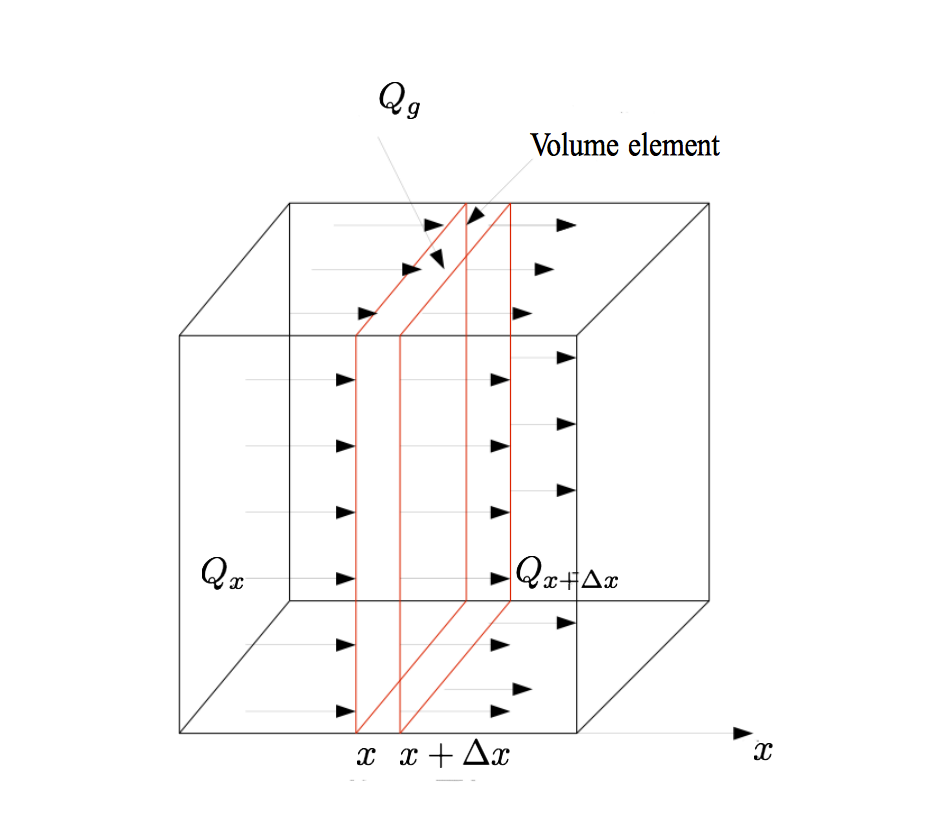
\includegraphics[width=0.5\textwidth]{heatcube.png}
}
\caption{\label{Fig_1DHeatConduction} One dimensional heat conduction through a volume element }
\end{center}
\end{figure}

The general heat transfer equation in 1D Cartesian coordinates can be obtained
from an energy balance on a volume element in Cartesian coordinates~\cite[page
34--36]{HeatConduction}.  Figure~\ref{Fig_1DHeatConduction} shows a thin
element of thickness $\Delta x$ on a large plate.

Energy balance on this element during small time interval $\Delta t$ is given
as:

\begin{equation}
\begin{split}
 \text{(Rate of heat transfer at }x) - \text{(Rate of heat transfer at }x+\Delta x) + \text{(Rate of heat} \\\text{generation inside the element)=(Rate of change of energy content of the element)}\label{eq:1}
\end{split}
\end{equation}

Using $Q$ for the rate of heat transfer and $E$ for the heat energy content,
this equation can be rewritten as:

\begin{equation}
Q_x- Q_{x+\Delta x} +Q_g=\frac{\Delta E}{\Delta t}, \label{eq:2}
\end{equation}

where $Q_x$ is the rate of heat transfer in the $x$ direction, $Q_g$ is rate of
heat generation inside the element and $\Delta E$ is the energy content of the
element.  If the volumetric heat generation in the element is $q'''$ and the
area of the plate is $A$, then the heat generated is:

\begin{equation}
Q_g=q'''A \Delta x \label{eq:3}
\end{equation}

The change in energy content of the element in time $\Delta t$ is
$\Delta E=E_{t+\Delta t}-E_t$

The temperature ($T$) can be introduced through the relation that $E=\rho C VT$,
where $\rho$ is the density, $C$ is the specific heat capacity and $V$ is the
volume of the element. In this case, $V=A\Delta x$.

\begin{equation}
 \Delta E=\rho C_p A\Delta x(T_{t+\Delta t}-T_t) \label{eq:4}
\end {equation}

Substituting \ref{eq:3}, \ref{eq:4} in \ref{eq:2}, 

\begin{equation}
Q_x -Q_{x+\Delta x} +q'''A\Delta x=\rho C A\Delta x\frac{T_{t+\Delta t}-T_t}{\Delta t} \label{eq:5}
\end{equation}

Dividing by $A\Delta x$ gives,

\begin{equation}
-(\frac{ Q_{x+\Delta x}-Q_x}{A \Delta x}) +q'''=\rho C \frac{T_{t+\Delta t}-T_t}{\Delta t} \label{eq:6}
\end{equation}

Taking the limit as $\Delta x \to 0$ and $\Delta t \to 0$ yields

\begin{equation}
-\frac{1}{A}\frac{\partial Q}{\partial x}+q'''=\rho C \frac{\partial T}{\partial t} \label{eq:7}
\end{equation}

According to Fourier's law, 

\begin{equation}
Q=-kA\frac{\partial T}{\partial x} \label{eq:8}
\end{equation}

substituting \ref{eq:8} into \ref{eq:7},

\begin{equation}
  -\frac{1}{A}\frac{\partial}{\partial x}(-kA\frac{\partial T}{\partial x}) +
  q''' = \rho C \frac{\partial T}{\partial t} \label{eq:9}
\end{equation}

\begin{equation}
  \frac{\partial}{\partial x}(k\frac{\partial T}{\partial x}) + q''' = \rho C
  \frac{\partial T}{\partial t}  \label{eq:10}
\end{equation}

If $k$ is temperature independent, then the above equation simplifies to:

\begin{equation} 
k\frac{\partial^2 T}{\partial x^2}+q'''=\rho C \frac{\partial T}{\partial t} \label{eq:11}
\end{equation}
~\newline

\noindent
\begin{bf}
Analogy between heat conduction and electrical conduction
\end{bf}
~\newline ~\newline

Figure~\ref{Fig_electricCircuit} shows the flow of current
in a circuit. From Ohm's law, we know that voltage ($V$) is directly
proportional to resistance ($R$) when current ($I$) is kept constant; that is,

\begin{equation}
V=IR
\end{equation}

When there are n resistors connected in series with resistances $R_1, R_2,
R_3,..... R_n$, the current ($I$) is same through each resistor. The, voltage
drop across all of the resistors is directly proportional to the effective
resistance ($R_e$).

\begin{equation}
V= IR_e,
\end{equation}

 where 

\begin{equation}
R_e=R_1+ R_2 + R_3.....+ R_n
\end{equation}
~\newline

\begin{figure}
\begin{center}
%\rotatebox{-90}
{
 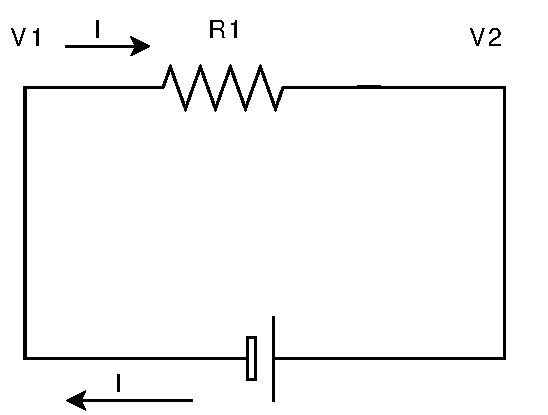
\includegraphics[width=0.5\textwidth]{electriccircuit.pdf}
}
\caption{Electric circuit}
\label{Fig_electricCircuit}
\end{center}
\end{figure}

Figure~\ref{Fig_ThermalCircuit} shows the heat flow in a slab.  The thermal
analogue of Ohm's law is written as,

\begin{equation}
\Delta T=QR_e \label{eq:12}
\end{equation}

That is, the temperature drop between the surfaces of a slab is directly
proportional to the thermal resistance between the surfaces, where $Q$ is the
rate of heat conduction.  From Fourier's law,

\begin{equation}
Q=-kA\frac{ dT}{ dx} \label{eq:13} 
\end{equation}

\begin{equation}
dT=-\frac{Q}{kA}dx \label{eq:14}
\end{equation}

Integrating LHS of \ref{eq:14} from $T_1$ to $T_2$ and RHS of \ref{eq:14} from
$x_1$ to $x_2$,

\begin{equation}
\int^{T_2}_{T_1}dT=-\frac{Q}{kA}\int^{x_2}_{x_1}dx \label{eq:15}
\end{equation}

\begin{equation}
\int^{T_1}_{T_2}dT=\frac{Q}{kA}\int^{x_2}_{x_1}dx  \label{eq:16}
\end{equation}

\begin{equation}
\int^{T_1}_{T_2}dT=\frac{Q}{kA}(x_2-x_1)  \label{eq:17}
\end{equation}

Since $x_2-x_1$ is the length of the element,

\begin{equation}
T_1-T_2=Q\frac{L}{kA} \label{eq:18}
\end{equation}

\begin{equation}
\Delta T=Q\frac{L}{kA} \label{eq:deltat}
\end{equation}

Comparing \ref{eq:12} with \ref{eq:deltat}, the resistance between the surfaces
is defined as,

\begin{equation}
 R_e=\frac{L}{kA}, \label{eq:reff}
\end{equation}

where $A$ is the effective area of the resistance and $k$ is the thermal conductivity.\\

\begin{figure}
\begin{center}
%\rotatebox{-90}
{
 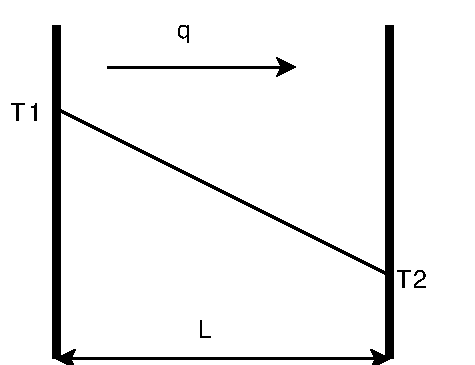
\includegraphics[width=0.5\textwidth]{heatcircuit.pdf}
}
\caption{Diagram representing heat flow in a slab}
\label{Fig_ThermalCircuit}
\end{center}
\end{figure}

\noindent

\begin{bf}
  Analogy between thermal capacitance and electrical capacitance
\end{bf}
~\newline

For electrical circuits, we have:

\begin{equation}
C\frac{dV}{dt}=I_{\text{in}}-I_{\text{out}}, \label{eq:C}
\end{equation} 

where $C$ is the capacitor,\\
$V$ is the voltage of the circuit,\\
$I_{\text{in}}$ and $I_{\text{out}}$ are the currents coming in and going out of the circuit respectively.\\
Equation~\ref{eq:C} is analogous to the heat transfer equation: 

\begin{equation}
C\frac{ dT}{dt} = q_{in}-q_{out}, \label{eq:34} 
\end{equation}

where $C$ is the capacitor,\\
$T$ is the temperature,\\
$q_{\text{in}}$ and $q_{\text{out}}$ are the heats coming in and going out of the circuit respectively.\\

\subsubsection{Terminology and  Definitions}

This subsection provides a list of terms that are used in the subsequent
sections and their meaning. This is provided with the purpose of reducing
ambiguity and making it easier to correctly understand the requirements:

\begin{itemize}

\item Decay heat: The heat released as a result of radioactive decay.

\item Delayed neutron: Neutron emitted by one of the fission products anytime
  from a few milliseconds to a few minutes later.

\item Delayed neutron precursors: Neutron-emitting fission fragments that
  undergo a stage of radioactive decay and yield an additional neutron called a
  delayed neutron.

\item Fuel pellet: a piece of nuclear fuel usually in the shape of a sphere or
  cylinder.

\item Flux depression: The lowering of the particle's flux density in the
  neighbourhood of an object due to absorption of particles in the object.

\item Heat Flux: The rate of heat energy transfer per unit area.

\item Linear Element power: The power generated per unit length of the fuelpin.

\item Prompt neutron: A neutron immediately emitted by a nuclear fission event.

\item Reactor trip: Emergency shutdown in the nuclear reactors.

\item Specific heat: heat capacity per unit mass

\item Thermal Capacitance: The amount of heat required to change a substance's
  temperature by a given amount.

\item Thermal Conduction: the transfer of heat energy through a substance.

\item Thermal Diffusivity: The thermal conductivity divided by density and
  specific heat capacity at constant pressure.

\item Thermal Resistance: Measure of a temperature difference by which an object
  or material resists a heat flow through it.

\item Transient: Changing with time.

\end{itemize}

\subsubsection{Physical System Description}

The physical system of the FP, as shown in
Figure~\ref{Fig_FuelpelletRepresentation} includes the following elements:

\begin{description}

\item[PS1:] Fuel pellet made of Uranium dioxide ($\mathrm{UO_2}$).

\item[PS2:] The clad material zircaloy covering the pellet.

\item[PS3:] Coolant surrounding the clad material.

\end{description}

NOTE: The temperatures $T_{\mathrm{CL}}$, $T_1$, $T_S$, $T_2$, $T_B$ in the
Figure~\ref{Fig_FuelpelletRepresentation} will be discussed later in this
document.

\begin{figure}
\begin{center}
%\rotatebox{-90}
{
 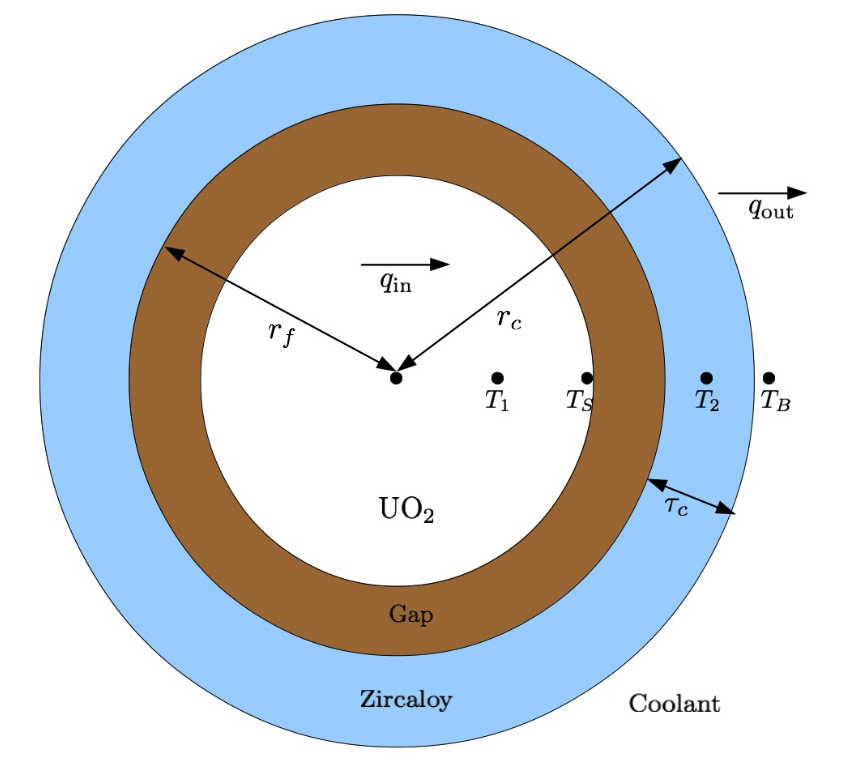
\includegraphics[width=0.5\textwidth]{fuelpin.png}
}
\caption{\label{Fig_FuelpelletRepresentation} Fuel pellet representation}
\end{center}
\end{figure}

\subsubsection{Goal Statements}

The goals of  FP are as follows:

\begin{description}

\item[G1:] Given fuel power versus time as input, predict transient reactor fuel
  and clad temperatures.

\item[G2:] Given the neutron flux versus time as input, predict transient
  reactor fuel and clad temperatures.

\item[G3:] Given the reactivity transient as input, predict transient reactor
  fuel and clad temperatures.

\item[G4:] Given the trip setpoints, number of trips to initiate shutdown,
  shutdown reactivity transient as inputs, simulate reactor trip and shutdown.
 
\end {description}

\subsection{Solution Characteristics Specification}

This section specifies the solution characteristics of the intended software
product. The purpose is to reduce the physical problem described in
Section~\ref{Sec_pd} to one expressed in mathematical terms. The section starts
with description of the assumptions that are made, and then describes the
theoretical models that are relevant for the FP problem. Data definitions,
instanced models, data constraints, and the expected system behaviour are also
given.

\subsubsection{Assumptions}

This section simplifies the original problem and helps in developing the
theoretical model by filling in the missing information for the physical
system. The numbers given in the square brackets refer to the data definition or
the instance model in which the respective assumption is used.

\begin{description}

\item[A\refstepcounter{assumpnum}\theassumpnum \label{A_axial}:] Axial
  conduction in the pellet is ignored [\dref{AvgTempOfCylinder}].

\item[A\refstepcounter{assumpnum}\theassumpnum \label{A_radial}:] The pellet has
  radial symmetry [\dref{AvgTempOfCylinder}].

\item[A\refstepcounter{assumpnum}\theassumpnum \label{A_kc}:] Averaged thermal
  conductivity value is considered [\ddref{DD_Rfuel}].

\item[A\refstepcounter{assumpnum}\theassumpnum \label{A_heidrick}:] The Urbanic,
  Heidrick model is used in modelling metal water reaction
  [\ddref{MetalWatReact}].

\item[A\refstepcounter{assumpnum}\theassumpnum \label{A_appr}:] Approximation of
  $\ln\frac{r_o}{r_i}$ as $\frac{\tau_c}{ r}$ and $r_o$ as $r_i$
  [\ddref{rclad}].

\item[A\refstepcounter{assumpnum}\theassumpnum \label{A_isotropic}:] Assume
  isotropic thermal conductivity [\tref {T_FL}].

\item[A\refstepcounter{assumpnum}\theassumpnum \label{A_coord}:] Cylindrical
  coordinate system is used [\dref{AvgTempOfCylinder}].

\item[A\refstepcounter{assumpnum}\theassumpnum \label{A_stk}:] The spacial
  effects are neglected in the reactor kinetics formulations
  [\iref{PointNeutronKinetics}].

\item[A\refstepcounter{assumpnum}\theassumpnum \label{A_Newtonfuel}:] Newton's
  law of convective cooling applies in the gap between the pellet surface and
  the clad [\ddref{rgap}].

\item[A\refstepcounter{assumpnum}\theassumpnum \label{A_Newtonclad}:] Newton's
  law of convective cooling applies between the clad surface and the coolant
  film[\ddref{rfilm}, \ddref{R2}].

\item[A\refstepcounter{assumpnum}\theassumpnum \label{A_rodlen}:] Unit length of
  fuel rod is being modelled [\dref{AvgTempOfCylinder}].

\item[A\refstepcounter{assumpnum}\theassumpnum \label{A_it2}:] Initially, the
  average clad temperature ($T_2$) is less than $1000^oC$.

\item[A\refstepcounter{assumpnum}\theassumpnum \label{A_tauc}:] The clad
  thickness ($\tau_c$) is constant even if the zircaloy is consumed in the metal
  water reaction.

\end{description}

\subsubsection{Theoretical Models}

This section focuses on the general equations, laws used to model a fuelpin.
~\newline

\noindent
\begin{minipage}{\textwidth}
\begin{tabular}{| p{\colAwidth} | p{\colBwidth}|}
  \hline
  \rowcolor[gray]{0.9}
  Number& T\refstepcounter{theorynum}\thetheorynum \label{T_COE}\\
  \hline
  Label&\bf Conservation of energy\\
  \hline
  Equation&  $-{\bf \nabla q} +q'''$ = $\rho C \frac{\partial T}{\partial t}$\\
  \hline
  Description & 
  The above equation gives the conservation
  of energy for a time varying heat transfer in a material of specific heat
  capacity $C$ and density $\rho$ where $\bf q$ is the thermal flux vector,
  $q'''$ is the volumetric heat generation, $T$ is the temperature and $\nabla$
  is the gradient operator. 
  \\
  \hline
\end{tabular}
\end{minipage}\\

~\newline
\noindent
\begin{minipage}{\textwidth}
\begin{tabular}{| p{\colAwidth} | p{\colBwidth}|}
\hline
\rowcolor[gray]{0.9}
Number& T\refstepcounter{theorynum}\thetheorynum \label{T_FL}\\
\hline
Label&\bf Constitutive Equation (Fourier's Law)\\
\hline
Equation&  ${\bf q}$=$-k(T){\bf\nabla} T$\\
\hline
Description & 
Fourier's law states that the heat flux  is propositional to slope or the
gradient of temperature, where $k$ is a function of temperature. This law is
based on the assumption that the material is isotropic (\aref{A_isotropic}).
\\
\hline
\end{tabular}
\end{minipage}\\

~\newline
\noindent
\begin{minipage}{\textwidth}
\begin{tabular}{| p{\colAwidth} | p{\colBwidth}|}
  \hline
  \rowcolor[gray]{0.9}
  Number & T\refstepcounter{theorynum}\thetheorynum \label{T_STK}\\
  \hline
  Label&\bf Space-Time kinetics\\
  \hline
  Equation&  Beyond the scope of this document.\\
  \hline
  Description & Space-Time kinetics give the relative distribution of the neutrons
  over space and time. 
  \\
  \hline
\end{tabular}
\end{minipage}\\

~\newline

\noindent
\begin{minipage}{\textwidth}
\begin{tabular}{| p{\colAwidth} | p{\colBwidth}|}
  \hline
  \rowcolor[gray]{0.9}
  Number & T\refstepcounter{theorynum}\thetheorynum \label{T_DHE}\\
  \hline
  Label&\bf Decay Heat Equations\\
  \hline
  Equation& Beyond the scope of this document.\\
  \hline
  Description & 
  Decay heat equations are used in finding the fuel power when neutron flux is
  given. It is a summation of the fuel power generated by prompt fissions and the
  fuel power generated by delayed decay heat components due to fission product
  decay.
  \\
  \hline
\end{tabular}
\end{minipage}\\

\subsubsection{General Definitions}

This section collects  the laws and equations that will be used in deriving the
data definitions, which in turn are used to  build the instance models.

\begin{figure}
\begin{center}
%\rotatebox{-90}
{
 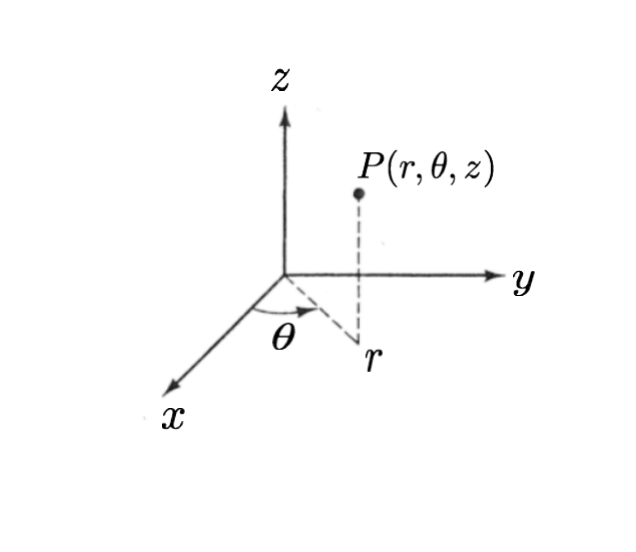
\includegraphics[width=0.5\textwidth]{Cylindrical-coordinates.png}
}
\caption{\label{Fig_COS} Cylindrical coordinate system}
\end{center}
\end{figure}

~\newline
\noindent
\begin{minipage}{\textwidth}
\begin{tabular}{| p{\colAwidth} | p{\colBwidth}|}
\hline
\rowcolor[gray]{0.9}
Number& GD\refstepcounter{defnum}\thedefnum \label{GradientInCylindCoord}\\
\hline
Label&\bf Cylindrical coordinate system\\
\hline
Units&-\\
\hline
SI equivalent &-\\
\hline
Equation & 
${\bf\nabla}=\hat{r}\frac{\partial}{\partial r} +
\hat{\theta}\frac{1}{r}(\frac{\partial}{\partial
  \theta})+\hat{z}\frac{\partial}{\partial z}$  where $\hat{r}$, $\hat{\theta}$
and $\hat{z}$ are unit vectors.
\\
& In matrix notation, this appears as:\\
& $ {\bf\nabla}=\begin{bmatrix}\frac{\partial}{\partial
    r}\\\frac{1}{r}\frac{\partial}{\partial \theta}\\\frac{\partial}{\partial
    z}\end{bmatrix}$
\\
& The divergence $ \mathrm{{\bf\nabla}A}$ is calculated as:\\
& $\mathrm{ {\bf\nabla}A}=\frac{\partial(A_r)}{\partial r}
+\frac{1}{r}\frac{\partial A_\theta}{\partial \theta}+\frac{\partial
  A_z}{\partial z}$
\\
\hline
Description & The spatial location in a cylindrical coordinate system is
expressed in terms of $\hat{r}$, $\hat{\theta}$, $\hat{z}$ as shown in the
Figure~\ref{Fig_COS}. The gradient operator is defined as shown above.
\\
\hline
 Sources & \cite[page 12]{FPManual}\\
\hline
\end{tabular}
\end{minipage}\\
~\newline

~\newline
\noindent
\begin{minipage}{\textwidth}
\begin{tabular}{| p{\colAwidth} | p{\colBwidth}|}
\hline
\rowcolor[gray]{0.9}
Number & GD\refstepcounter{defnum}\thedefnum \label{AvgTempOfCylinder}\\
\hline
Label &\bf Average temperature of a hollow cylinder\\
\hline
Units&$M^0L^0t^0T$\\
\hline
SI equivalent &$^oC$\\
\hline
Symbol &$ T_{\mathrm{AVG}}$\\
\hline
Equation & $ T_{\mathrm{AVG}}= \frac{1}{A} \int_{A} T(r)dA$, with $T(r)$ satisfying 
$\frac{1}{r} \frac{d}{dr} (kr \frac{dT(r)}{dr})+q''' = 0$
\\
\hline
Description & $T_{\mathrm{AVG}}$ is the average temperature of the cylinder, $A$
is the area of the cylinder and $T(r)$ is the temperature at radius $r$.
\\
\hline
\end{tabular}
\end{minipage}\\

\begin{bf}
~\newline
{Detailed derivation of average temperature:}\\
\end{bf}

\noindent
 Applying the Fourier's law from TM2 to Conservation of energy equation in TM1,
 gives 

\begin{equation}
\nabla k \nabla T + q''' = \rho C \frac{\partial T}{\partial t} \label{Eq_Avg}
\end{equation}

In steady state, the transient features die and (29) changes to

\begin{equation}
 \nabla k \nabla T + q''' =0
\end{equation}

 Applying \aref{A_coord} and writing the above  equation in cylindrical
 coordinate system (\dref{GradientInCylindCoord}),

\begin{equation}
 k [\frac{1}{r}\frac{\partial}{\partial r}(r\frac{\partial T}{\partial r}) +
 \frac{1}{r^2}\frac{\partial}{\partial \theta}(\frac{\partial T}{\partial
   \theta})+\frac{\partial}{\partial z}(\frac{\partial T}{\partial z})]+ q'''= 0
\end{equation}

Ignoring axial conduction (\aref{A_axial}), makes 
$\frac{1}{r^2}\frac{\partial}{\partial \theta}(k\frac{\partial T}{\partial
  \theta})=0$.

and having radial symmetry (\aref{A_radial}) makes $\frac{\partial}{\partial
  z}(k\frac{\partial T}{\partial z})=0$.

So, applying
 \aref{A_axial} and \aref{A_radial} to (31),  it simplifies to:

\begin{equation}
\frac{1}{r} \frac{d}{dr} (kr \frac{dT}{dr})+q''' = 0 \label{eq_tr}
\end{equation}

Average temperature of the hollow cylinder is found by taking the volume
averaged value of the temperature at radius $r$. Let $r_1$ be the inner radius
and $r_2$ be the outer radius of a hollow cylinder. Then the average temperature
of the cylinder is given by

\begin{equation}
T_{\mathrm{AVG}}=\frac{\int _V T(r,z,\theta)dV}{V}
\end{equation}

\noindent
Taking \aref{A_axial} and \aref{A_radial} and \aref{A_rodlen}  into account, 

\begin{equation}
 T_{\mathrm{AVG}}=\frac{1}{A} \int_{A} T(r)dA
\end{equation}

~\newline
\noindent
\begin{minipage}{\textwidth}
\begin{tabular}{| p{\colAwidth} | p{\colBwidth}|}
\hline
\rowcolor[gray]{0.9}
Number & GD\refstepcounter{defnum}\thedefnum \label{EffectThermResist}\\
\hline
Label &\bf Effective thermal resistance\\
\hline
Symbol & $ R_{\text{EFF}}$\\
\hline
Units & $M^{-1}L^{-2}Tt^{3}$\\
\hline
SI equivalent & $\mathrm{\frac{m^oC}{kW}}$\\
\hline
Equation & $ R_{\mathrm{EFF}}= \frac {\Delta T}{q}$\\
\hline
Description & 
In some cases at steady state, the relation between the temperature change
($\Delta$T)  and the thermal flux ($q$) is modelled as $\Delta$T being directly
proportional to $q$. The proportionality constant can be derived using
thermodynamic theory and then relabelled as $R_{\mathrm{EFF}}$. This is
analoguos to the electric circuit equation of $V$=$IR$.
\\
& As for the case of electric resistors in series, if $n$ resistors
$(R_1,R_2.....R_n)$ are connected in series between two temperatures and if
constant heat is flowing between those temperatures, then $ R_{\mathrm{EFF}}=
R_1+R_2+....+R_n$ 
\\
\hline
\end{tabular}
\end{minipage}\\

~\newline
\noindent
\begin{minipage}{\textwidth}
\begin{tabular}{| p{\colAwidth} | p{\colBwidth}|}
\hline
\rowcolor[gray]{0.9}
Number& GD\refstepcounter{defnum}\thedefnum \label{TRCE}\\
\hline
Label &\bf Rate of change of temperature \\
\hline
Equation&$C \frac{dT_{\mathrm{AVG}}}{dt} = q_{\mathrm{in}}-q_{\mathrm{out}}+q_g$  \\
\hline
Description & The basic equation governing the rate of change of temperature with time.\\
& where $C$ is the thermal capacitance ($\frac{\mathrm{kW}s}{m^oC}$) \\
& $q_{\mathrm{in}},q_{\mathrm{out}}$ are the linear in and out heat transfer
rates respectively ($\frac{\mathrm{kW}}{m}$) and $q_g$ is the rate of internal
heat generated.
\\
\hline
\end{tabular}
\end{minipage}\\

\begin{bf}
~\newline
{Detailed derivation of Rate of change of temperature  :}\\
\end{bf}

Integrating \tref{T_COE} over the volume ($V$),

\begin{equation}
-\int_V{\bf \nabla q} dV+\int_V q''' dV= \int_V \rho C \frac{\partial T}{\partial t}dV
\end{equation}

Applying Gauss's Divergence theorem to the first term over surface $S$,

\begin{equation}
-\int_S{ \bf{q\cdot \hat n}} dS+\int_V q''' dV= \int_V \rho C \frac{\partial T}{\partial t}dV
\end{equation}

Taking \aref{A_rodlen} into consideration,  the volume average gets changed to
area average. 

\begin{equation}
 -\int_S{ \bf{q\cdot \hat n}} dS+\int_A q''' dA= \int_A \rho C \frac{\partial T}{\partial t}dA \label{eq:43}
\end{equation}

Consider a hollow cylinder as in Figure~\ref{Fig_heat}. The integral over the
surface can be summarized as $q_{in}-q_{out}$. The integral of $q'''$ over the
area becomes the generated thermal energy $q'_g$. Hence (\ref{eq:43}) can be
written as,

\begin{equation}
  q_{\mathrm{in}}-q_{\mathrm{out}}+q_g= \int_A \rho C \frac{\partial T}{\partial t}dA \label{eq:44}
\end{equation}

Taking the time derivative of \dref{AvgTempOfCylinder}.

\begin{equation}
\frac{ dT_{\mathrm{AVG}}}{dt}= \frac{1}{A} \int_{A} \frac{dT}{dt}dA
\end{equation}

Rearranging the above equation,

\begin{equation}
A\frac{ dT_{\mathrm{AVG}}}{dt}= \int_{A} \frac{dT}{dt}dA
\end{equation}

 Assuming there are representative values of specific heat ($c_p$) and density
 ($\rho$) and multiplying the above equation with $\rho C_{rep}$:

\begin{equation}
\rho C_{rep} A\frac{dT_{\mathrm{AVG}}}{dt} =  \int_A \rho C_{rep} \frac{\partial T}{\partial t}dA \label{eq:46}
\end{equation}

Replacing the RHS of (\ref{eq:44}) with the LHS of (\ref{eq:46}),

\begin{equation}
\rho C_{rep} A\frac{dT_{\mathrm{AVG}}}{dt} = q_{\mathrm{in}}-q_{\mathrm{out}}+q_g \label{eq:TAV}
\end{equation}

\begin{figure}
\begin{center}
%\rotatebox{-90}
{
 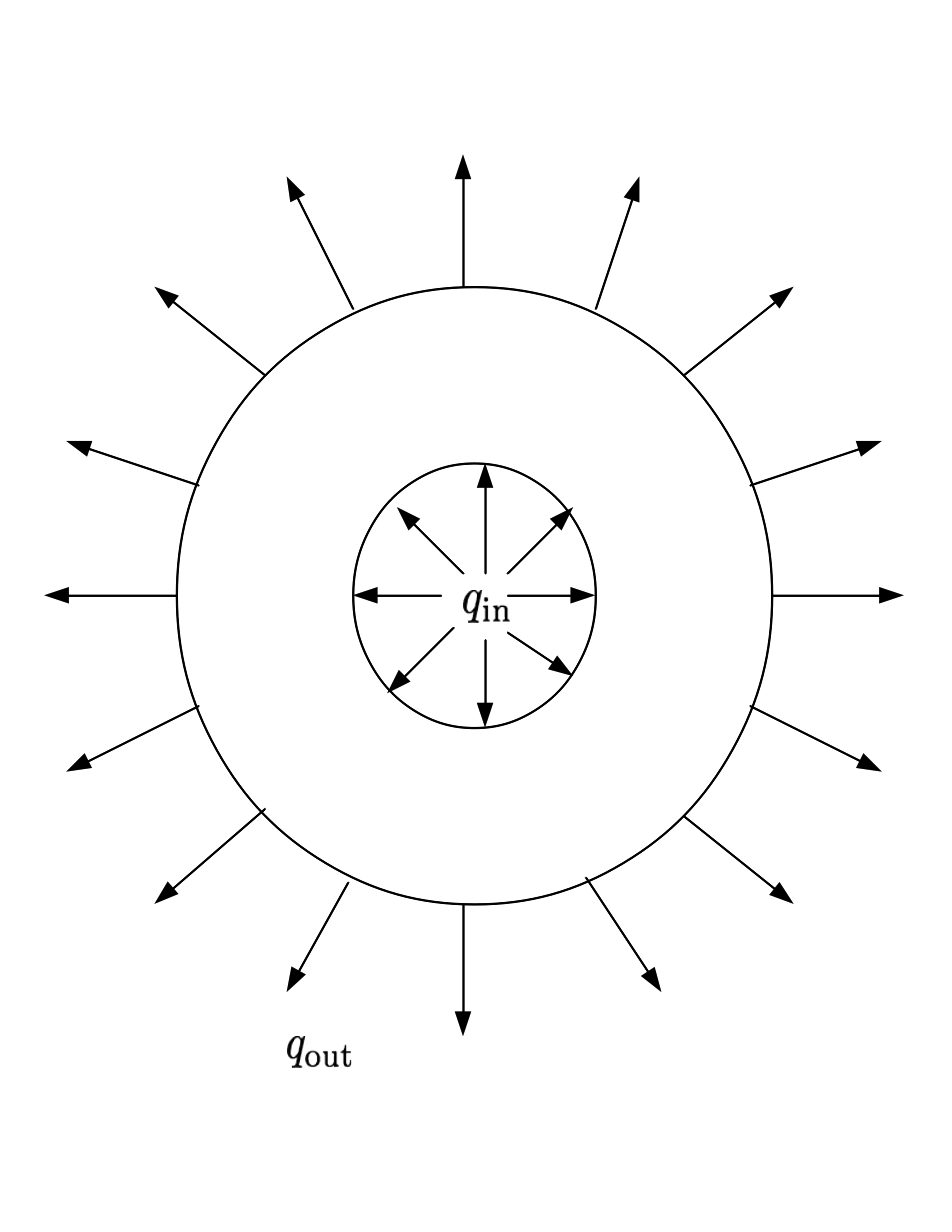
\includegraphics[width=0.4\textwidth]{heat.png}
}
\caption{\label{Fig_heat} Heat transfer in a hollow cylinder}
\end{center}
\end{figure}

~\newline
\noindent
\begin{minipage}{\textwidth}
\begin{tabular}{| p{\colAwidth} | p{\colBwidth}|}
\hline
\rowcolor[gray]{0.9}
Number& GD\refstepcounter{defnum}\thedefnum \label{NL}\\
\hline
Label &\bf Newton's law of cooling \\
\hline
Units&$MLt^{-3}T^0$\\
\hline
SI equivalent&$\mathrm{\frac{kW}{m}}$\\
\hline
Equation&$ q_{\text{newt}}= h A \Delta T(t)$  \\
\hline
Description &
Newton's law of cooling describes the convection cooling and is stated as ``rate
of heat loss of a body is proportional to the difference in temperatures between
the body and its surroundings.''
\\
& $q_{\text{newt}}$ is the thermal flux.\\
& $h$ is the heat transfer coefficient (assumed independent of $T$ here)
($\frac{\text{W}}{\text{m}^2\text{K}}$)
\\
&  $A$ is the surface area of the heat being transferred ($\text{m}^2$)\\
 &$\Delta T(t)$= $T(t) - T_{\text{env}}$ is the time-dependent thermal gradient
 between environment and object. Newton's law of cooling can be derived from
 Fourier's law (\tref{T_FL})
\\
\hline
\end{tabular}
\end{minipage}\\

~\newline
\noindent
\begin{minipage}{\textwidth}
\begin{tabular}{| p{\colAwidth} | p{\colBwidth}|}
\hline
\rowcolor[gray]{0.9}
Number& GD\refstepcounter{defnum}\thedefnum \label{ehtc}\\
\hline
Label &\bf Effective heat transfer coefficient \\
\hline
Units&$M^{-1}L^{2}t^{-3}T^{-1}$\\
\hline
SI equivalent&$\frac{\text{W}}{\text{m}^2\text{K}}$\\
\hline
Equation&$  h_{\text{EFF}} =\frac{q}{A \Delta T(t)}$  \\
\hline
Description 
& $q$ is the thermal flux.\\
& $h_{\text{EFF}}$ is the effective heat transfer coefficient ($\frac{\text{W}}{\text{m}^2\text{K}}$)\\
& $A$ is the surface area of the heat being transferred ($\text{m}^2$)\\
& $\Delta T(t)$= $T(t) - T_{\text{env}}$ is the time-dependent thermal gradient
between environment and object.
\\
& The heat transfer coefficient is modelled after Newton's law of cooling. It
takes into account all relevant modes of heat transfer.
\\ 
\hline
\end{tabular}
\end{minipage}\\

\subsubsection{Data Definitions}

This section collects and defines all the data needed to build the instance
models. The dimension of each quantity is also declared.

~\newline

\noindent
\begin{minipage}{\textwidth}
\begin{tabular}{| p{\colAwidth} | p{\colBwidth}|}
\hline
\rowcolor[gray]{0.9}
Number& DD\refstepcounter{datadefnum}\thedatadefnum \label{LinearElmPower}\\
\hline
Label& \bf Relation between linear element power and volumetric heat generation\\
\hline
Symbol &$ q'_N$\\
\hline
Units&$MLt^{-3}T^0$\\
\hline
SI equivalent &$\mathrm{\frac{kW}{m}}$\\
\hline
Equation&$q'_N=\pi r_f^2q'''$\\
\hline
Description & 
$q'''$ is the volumetric heat generation and $r_f$ is the fuel radius. The
linear element power ($q'_N$) is found by multiplying the volumetric heat
generation by the cross-sectional area of the fuel element. 
\\
\hline
 Sources& \cite[page 2--3]{FPManual}; \\
\hline
\end{tabular}
\end{minipage}\\

~\newline

~\newline

\noindent
\begin{minipage}{\textwidth}
\begin{tabular}{| p{\colAwidth} | p{\colBwidth}|}
  \hline
  \rowcolor[gray]{0.9}
  Number& DD\refstepcounter{datadefnum}\thedatadefnum \label{FuelStoredEnergy}\\
  \hline
  Label&\bf Fuel stored energy\\
  \hline
  Symbol &$\Delta H (T_{\text{abs}})$\\
  \hline
  Units&$M^0L^2t^{-2}T^0$\\
  \hline
  SI equivalent &$\mathrm{\frac{J}{kg}}$\\
  \hline
  Equation & $\Delta H (T_{\text{abs}})$ = $K_0(K_1 \theta
  ((e^{\frac{\theta}{T_{\text{abs}}}}-1)^{-1} - (e^{\frac{\theta}{298}}-1)^{-1} )+
  K_2 (T_{\text{abs}}^2-298^2) + K_3 e^ {\frac{-E_D}{R_DT_{\text{abs}}}})$
  \\
  \hline
  Description & 
  The stored energy ($\Delta H (T_{\text{abs}})$) calculated is the change in
  fuel enthalpy from room temperature $(298 ^oK)$ to the absolute value of the
  average fuel temperature $T_1$ ($T_{\text{abs}}$).  The values of the 
  constants are given by the Table~\tbref{fse}
  \\
  \hline
  Sources& \cite[page 12]{FPManual}; \\
  \hline
\end{tabular}
\end{minipage}\\
~\newline

~\newline
\noindent
\begin{minipage}{\textwidth}
\begin{tabular}{| p{\colAwidth} | p{\colBwidth}|}
\hline
\rowcolor[gray]{0.9}
Number & DD\refstepcounter{datadefnum}\thedatadefnum \label{IntegFuelPow}\\
\hline
Label&\bf Integrated fuel power\\
\hline
Symbol&$P_{\mathrm{F,SUM}} $\\
\hline
Units&FPS\\
\hline
SI equivalent &-\\
\hline
Equation&$P_{\mathrm{F,SUM}}(t_i) $=  $\int_{0} ^{t_i} q'_{\text{NFRAC}}(t) dt$\\
\hline
Description &
The above equation gives the integrated fuel power at $t_i$, where
$q'_{\text{NFRAC}}$ is the relative fuel power and $P_{\mathrm{F,SUM}}(t_i)$ is the integrated fuel power at $t_i$ 
\\
\hline
 Sources& \cite[page 12]{FPManual}; \\
\hline
\end{tabular}
\end{minipage}\\
~\newline

~\newline
\noindent
\begin{minipage}{\textwidth}
\begin{tabular}{| p{\colAwidth} | p{\colBwidth}|}
\hline
\rowcolor[gray]{0.9}
Number& DD\refstepcounter{datadefnum}\thedatadefnum \label{TempFeedbackReact}\\
\hline
Label&\bf Temperature feedback reactivity\\

\hline
Symbol &$ \rho_{\mathrm{TFB,i}}$\\
\hline
Units&-\\
\hline
SI equivalent &mk\\
\hline
Equation&$ \rho_{\mathrm{TFB,i}}$ = $A (T_{1,i}-T_{1,0} )$\\
\hline
Description & $ A$ is a constant $(\frac{\mathrm{mk}}{\mathrm{^oC}})$ and
$T_{1,0}$ as the initial average temperature $(\mathrm{^oC})$
\\
\hline
 Sources& \cite[page 11]{FPManual}; \\
\hline
\end{tabular}
\end{minipage}\\
~\newline

~\newline
\noindent
\begin{minipage}{\textwidth}
\begin{tabular}{| p{\colAwidth} | p{\colBwidth}|}
\hline
\rowcolor[gray]{0.9}
Number& DD\refstepcounter{datadefnum}\thedatadefnum \label{MetalWatReact}\\
\hline
Label&\bf Metal water reaction\\
\hline
Symbol &$q'_{\mathrm{MWR}}$\\
\hline
Units&$MLt^{-3}T^0$\\
\hline
SI equivalent &$\mathrm{\frac{kW}{m}}$\\
\hline
Equation&${R_{\text{ox}}}$ = $[\frac{A}{1.56  \delta_{\text{ox}}}] e^{\frac{-B}{R(T_2+273)}}      $\\
& if
($\delta_{\text{ox}}\geq \tau_c $)\\
&\ $q'_{\text{MWR}}=0$\\
&else\\
&\ $q'_{\mathrm{MWR}}$= ${R_{\text{ox}}} 2\pi r_c  \rho_2 q_r $\\
\hline
Description & $\delta_{\text{ox}}$  is the reacted zircaloy thickness (m)\\
&$R_{\text{ox}}$ is the rate of oxidization\\
&$ q'_{\mathrm{MWR}}$ is the metal water reaction heat ($\mathrm{\frac{kW}{m}}$)\\
&$\rho_2$ is the clad density ($\mathrm{\frac{kg}{m^3}}$)\\
&$r_c$ is the clad radius\\
&$\tau_c$ is the clad thickness\\
&$T_2$ is the average clad temperature\\
&$q_r$ is the heat of reaction ($\mathrm{\frac{kJ}{kg}}$) and its value is given in (\tbref{mwr})\\
&$A$,  $B/R$ are constants with their values given in (\tbref{mwr})\\ 
& The Urbanic, Heidrick model is used to predict the oxidation rate from the
parabolic rate law (\aref{A_heidrick})\\
\hline
Sources& \cite[page 11]{FPManual}\\
\hline
\end{tabular}
\end{minipage}\\

~\newline
\noindent
\begin{minipage}{\textwidth}
\begin{tabular}{| p{\colAwidth} | p{\colBwidth}|}
\hline
\rowcolor[gray]{0.9}
Number & DD\refstepcounter{datadefnum}\thedatadefnum \label{DD_Rfuel}\\
\hline
Label&\bf Effective thermal resistance of fuel\\

\hline
Symbol &$ R_{\mathrm{FUEL}}$\\
\hline
Units&$M^{-1}L^{-2}t^{3}T$\\
\hline
SI equivalent &$\mathrm{\frac{m^oC}{kW}}$\\
\hline
Equation&$ R_{\mathrm{FUEL}}= \frac {f}{4 \pi k_{\mathrm{AV}}}$\\
\hline
Description & 
$R_{\mathrm{FUEL}}$ is the effective thermal resistance between the temperatures
$T_{\mathrm{CL}}$ and $T_S$. 
\\
& $\frac{R_{\mathrm{FUEL}}}{2}$ is the effective thermal resistance between
$T_{\mathrm{CL}}$ and $T_1$ and between $T_1$ and $T_S$
\\
&$f$ is the flux depression factor\\
&$ k_{\mathrm{AV}}$ is the average fuel conductivity\\
\hline
 Sources& \cite[page 3]{FPManual}; \\
\hline
\end{tabular}
\end{minipage}
~\newline

~\newline
\begin{bf}
  Detailed derivation of $R_{\mathrm{FUEL}}$: \\
\end{bf}
~\newline

\noindent
From  Equation~\ref{eq_tr} of (\dref{AvgTempOfCylinder}),

\begin{equation}
  \frac{1}{r} \frac{d}{dr} (kr \frac{dT}{dr})+q''' = 0 
\end{equation}

Integrating and rearranging the above equation gives:

\begin{equation}
  kr \frac{dT}{dr} = -\int^r_0 rq''' dr
\end{equation}

\begin{equation}
  \Rightarrow kr \frac{dT}{dr} =\frac{-q'''r^2}{2} 
\end{equation}

\begin{equation}
  \Rightarrow k\frac{dT}{dr} =\frac{-q'''r}{2}
\end{equation}

\begin{equation}
  \Rightarrow k dT =\frac{-q'''r}{2} dr \label{eq:53}
\end{equation}

For a fuel pellet with outer radius $r_f$, integrating the RHS of (\ref{eq:53})
from 0 to $r_f$ and LHS of (\ref{eq:53}) from $T_{\mathrm{CL}}$ to $T_S$,

\begin{equation}
\int^{T_S}_{T_{\mathrm{CL}}} dT= \frac{-q'''}{2}\int^{r_f}_{0}\frac{r}{k}dr \label{eq:54}
\end{equation}

\begin{equation}
\Rightarrow T_{S} - T_{\mathrm{CL}}=\Delta T = -q'''\frac{r_f^2}{4k} \label{eq:55}
\end{equation}

Multiplying both sides of (\ref{eq:55}) by minus sign,

\begin{equation}
T_{\mathrm{CL}} - {T_S}=\Delta T = q'''\frac{r_f^2}{4k} \label{eq:56}
\end{equation}

Applying \aref{A_kc} to (\ref{eq:56}),

\begin{equation}
{T_{\mathrm{CL}}} - {T_S}=\Delta T = q'''\frac{r_f^2}{4k_{\mathrm{AV}}} \label{eq:57}
\end{equation}

Replacing the volumetric heat generation by the linear element power using the
relation from \ddref{LinearElmPower}, removes the dependence of $\Delta T$ on
the pellet radius. Rewriting (\ref{eq:57}),\\

\begin{equation}
T_{\mathrm{CL}}-T_S=\frac{q'_N}{4\pi k_{\mathrm{AV}}} \label{eq:58}
\end{equation}

Taking flux depression factor ($f$) of the fuel pellet into consideration,
(\ref{eq:58})  can be written as,

\begin{equation}
 T_{\mathrm{CL}}-T_S=\Delta T=(\frac{f }{4\pi k_{\mathrm{AV}}})q'_N \label{eq:tcl}
\end{equation}

\noindent 
Comparing the above equation to (\dref{EffectThermResist}) shows that the
effective thermal resistance, $R_{\mathrm{FUEL}}$ in this case, is:

\begin{equation}
 R_{\mathrm{FUEL}}=\frac {f}{4 \pi k_{\mathrm{AV}}}
\end{equation}

\noindent
\begin{minipage}{\textwidth}
\begin{tabular}{| p{\colAwidth} | p{\colBwidth}|}
\hline
\rowcolor[gray]{0.9}
Number& DD\refstepcounter{datadefnum}\thedatadefnum \label{rclad}\\
\hline
Label&\bf $R_{\mathrm{CLAD}}$\\
\hline
Units&$M^{-1}L^{-2}t^{3}T$\\
\hline
SI equivalent &$\mathrm{\frac{m^oC}{kW}}$\\
\hline
Equation& $R_{\mathrm{CLAD}}=\frac{\tau_c}{2\pi r_ck_c}$\\
\hline
Description & The clad resistance is a function of the clad thermal conductivity. It
is obtained from the expression for heat transfer by conduction through a
hollow cylinder with inner radius $r_i$ and outer radius $r_o$ where
$k_c$ is the clad conductivity ($\mathrm{\frac{kW}{m^oC}}$) and is given as, $
\frac{\Delta T}{q}$=$\frac{\ln {\frac{r_o}{r_i}}}{2\pi k_c}$
\\
& Taking \aref{A_appr} into consideration, we get $  \frac{\Delta T}{q}$=
$\frac{\tau_c}{2\pi r_ck_c}$
\\
& Comparison to \dref{EffectThermResist}, shows that effective thermal resistance
 $R_{\mathrm{CLAD}}=\frac{\tau_c}{2\pi r_ck_c}$ 
\\
\hline
 Sources& \cite[page 4]{FPManual}, \cite[page 5]{HollowCylinder} ; \\
\hline
\end{tabular}
\end{minipage}\\

~\newline
\noindent
\begin{minipage}{\textwidth}
\begin{tabular}{| p{\colAwidth} | p{\colBwidth}|}
\hline
\rowcolor[gray]{0.9}
Number & DD\refstepcounter{datadefnum}\thedatadefnum \label{rgap}\\
\hline
Label&\bf$ R_{\mathrm{GAP}}$\\
\hline
Units&$M^{-1}L^{-2}t^{3}T$\\
\hline
SI equivalent &$\mathrm{\frac{m^oC}{\text{kW}}}$\\
\hline
Equation&$R_{\mathrm{GAP}}$ = $\frac{1}{2\pi r_c h_p} $\\
\hline
Description & $R_{\mathrm{GAP}}$ is the gap resistance  where
$r_c$ is the clad radius (m),
$h_p$ is the initial gap conductance ($\mathrm{\frac{kW}{m^{2o}C}}$) which is an
input parameter
\\
\hline
 Sources& source code \\
\hline
\end{tabular}
\end{minipage}\\
~\newline

\begin{bf}
  Derivation of
\end{bf} $R_{\text{GAP}}$

~\newline 

Taking \aref{A_Newtonfuel} into consideration, we use Newton's law of cooling to
derive $R_{\text{GAP}}$.  The area of the clad ($A_c$) is

\begin{equation}
  A_c= 2 \pi r_c \label{areag}
\end{equation}

Substituting Equation~\ref{areag} into \dref{NL}, and considering $h_p$ as the
initial gap conductance (heat transfer coefficient), we get,

\begin{equation}
q_{\text{gap}}=  2\pi r_c h_p \Delta T \label{newtg}
\end{equation}

From \dref{EffectThermResist}, the gap resistance ($R_{\mathrm{GAP}}$) can be
given as, 

\begin{equation}
R_{\mathrm{GAP}}=\frac{\Delta T}{q_{\text{gap}}} \label{gap}
\end{equation}

Substituting Equation~\ref{newtg} into Equation~\ref{gap} and simplifying gives,

\begin{equation}
R_{\mathrm{GAP}}=\frac{1}{2\pi r_c h_p}
\end{equation} 

~\newline
\noindent
\begin{minipage}{\textwidth}
\begin{tabular}{| p{\colAwidth} | p{\colBwidth}|}
  \hline
  \rowcolor[gray]{0.9}
  Number& DD\refstepcounter{datadefnum}\thedatadefnum \label{rfilm}\\
  \hline
  Label&\bf$ R_{\mathrm{FILM}}$\\
  \hline
  Units&$M^{-1}L^{-2}t^{3}T$\\
  \hline
  SI equivalent &$\mathrm{\frac{m^oC}{\text{kW}}}$\\
  \hline
  Equation&$R_{\mathrm{FILM}}$ = $\frac{1}{2\pi r_c h_b} $\\
  \hline
  Description&$R_{\mathrm{FILM}}$ is the coolant film resistance  where
  $r_c$ is the outer clad radius (m),
  $h_b$ is the coolant film conductance ($\frac{\text{kW}}{m^2C})$ (Figure~\ref{Fig_ElectCirc2})\\
  &NOTE: Equation taken from the code\\
  \hline
  Sources& source code \\
  \hline
\end{tabular}
\end{minipage}\\
~\newline

\begin{figure}
\begin{center}
%\rotatebox{-90}
{
 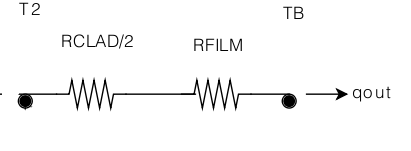
\includegraphics[width=0.4\textwidth]{electricalcircuit2.png}
}
\caption{\label{Fig_ElectCirc2} Thermal circuit between $T_2$ and $T_B$}
\end{center}
\end{figure}

\begin{bf}
Derivation of $R_{\text{FILM}}$
\end{bf}

~\newline Assuming that Newton's law of convective cooling applies between the
clad and the coolant ( \aref{A_Newtonclad}), we use Newton's law of cooling to
derive $R_{\text{FILM}}$.  The area of the clad ($A_c$) is

\begin{equation}
A_c= 2 \pi r_c \label{area}
\end{equation}

Substituting Equation~\ref{area} into \dref{NL}, and considering $h_b$ as the
coolant film conductance, we get,

\begin{equation}
q_{\text{coolant}}=  2\pi r_c h_b \Delta T \label{eq:newtc}
\end{equation}

From \dref{EffectThermResist}, the coolant film resistance ($R_{\mathrm{FILM}}$)
can be given as, 

\begin{equation}
R_{\mathrm{FILM}}=\frac{\Delta T}{q_{\text{coolant}}} \label{cool}
\end{equation}

Substituting Equation~\ref{eq:newtc} in Equation~\ref{cool} and simplifying
gives,

\begin{equation}
R_{\mathrm{FILM}}=\frac{1}{2\pi r_c h_b}
\end{equation} 

\noindent
\begin{minipage}{\textwidth}
\begin{tabular}{| p{\colAwidth} | p{\colBwidth}|}
  \hline
  \rowcolor[gray]{0.9}
  Number& DD\refstepcounter{datadefnum}\thedatadefnum \label{r3}\\
  \hline
  Label&\bf$ R_3$\\
  \hline
  Units&$M^{-1}L^{-2}t^{3}T$\\
  \hline
  SI equivalent &$\mathrm{\frac{m^oC}{kW}}$\\
  \hline
  Equation&$R_3$ = $\frac{1}{2\pi r_f h_g}$\\
  \hline
  Description & 
  $R_3$ is the effective thermal resistance between $T_S$ and $T_2$ (Figure~\ref{Fig_ElectCirc2}) where
  $r_f$ is the fuel radius (m) $h_g$ is the gap film conductance (kw/$m^2$$^oC$)
  which is given by \ddref{hg}
  \\
  \hline
  Sources& \cite[page 5]{FPManual}\\
  \hline
\end{tabular}
\end{minipage}\\
~\newline

\begin{bf}
Detailed derivation of $R_3$:
\end{bf}

~\newline
From Figure~\ref{Fig_ThermCirc1to2}, the effective resistance $R_3$ between
$T_S$ and $T_2$ is: 

\begin{equation}
R_3=R_{\mathrm{GAP}} + \frac{R_{\mathrm{CLAD}}}{2} \label{r3e}
\end{equation}

From \dref{EffectThermResist}, the heat flux between the fuel surface and clad
can be given as,

\begin{equation}
q=\frac{\Delta T}{R_3}, \label{rgq}
\end{equation} 

Taking $h_g$ as the effective heat transfer coefficient between fuel surface and
clad, we get the heat flux between the fuel surface and clad from \dref{ehtc} as

\begin{equation}
q=h_g A_f \Delta T, \label{rgn}
\end{equation}

where $A_f$ is the area of the clad given as

\begin{equation}
A_f=2 \pi r_f \label{areaf}
\end{equation}

Comparing Equation~\ref{rgn} and Equation~\ref{rgq},

\begin{equation}
\frac{\Delta T}{R_3}=h_g A_f \Delta T
\end{equation}

Replacing $A_f$ with its value from Equation~\ref{areaf} and further
simplifying, we get,

\begin{equation}
R_3=\frac{1}{ 2\pi r_fh_g}
\end{equation}

\begin{figure}[h!]
\begin{center}
%\rotatebox{-90}
{
 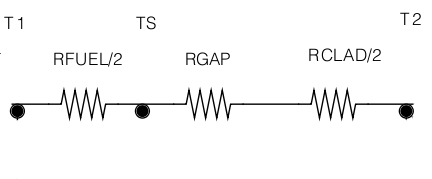
\includegraphics[width=0.4\textwidth]{electricalcircuit.png}
}
\caption{\label{Fig_ThermCirc1to2} Thermal circuit between $T_1$ and $T_2$}
\end{center}
\end{figure}

~\newline
\noindent
\begin{minipage}{\textwidth}
\begin{tabular}{| p{\colAwidth} | p{\colBwidth}|}
  \hline
  \rowcolor[gray]{0.9}
  Number& DD\refstepcounter{datadefnum}\thedatadefnum \label{R1}\\
  \hline
  Label&\bf$ R_1$\\
  \hline
  Units&$M^{-1}L^{-2}t^{3}T$\\
  \hline
  SI equivalent &$\mathrm{\frac{m^oC}{kW}}$\\
  \hline
  Equation&$R_1 = \frac{f}{8\pi k_{\mathrm{AV}}} + \frac{1}{2\pi r_f h_g} $\\
  \hline
  Description & 
  $R_1$ is the thermal resistance between the average fuel temperature ($T_1$) and clad temperature ($T_2$)
  (Figure~\ref{Fig_ThermCirc1to2})
  \\
  &$ k_{\mathrm{AV}}$ is the average fuel conductivity\\
  &$r_f$ is the fuel radius (m)\\
  &$h_g$ is the gap film conductance (kw/$m^2$$^oC$) which is given by \ddref{hg}\\
  \hline
  Sources& \cite[page 4]{FPManual}; \\
  \hline
\end{tabular}
\end{minipage}\\
~\newline

\begin{bf}
  Derivation of $R_1$:
\end{bf}

~\newline
From the Figure~\ref{Fig_ThermCirc1to2}, the effective resistance $R_1$ between
$T_1$ and $T_2$ is: 

\begin{equation}
R_1 = \frac{R_{\mathrm{FUEL}}}{2} + R_{\mathrm{GAP}} + \frac{R_{\mathrm{CLAD}}}{2}
\end{equation}

From Equation~\ref{r3e}, since $R_3$ is the effective resistance of gap and half
of the clad, the above equation can be rewritten as,

\begin{equation}
R_1 = \frac{R_{\mathrm{FUEL}}}{2} + R_3 \label{r1e}
\end{equation}

Substituting the values of $R_{\mathrm{FUEL}}$, $R_3$ from \ddref{DD_Rfuel} and
\ddref{r3} respectively into Equation~\ref{r1e} gives:

\begin{equation}
R_1 = \frac{f}{8\pi k_{\mathrm{AV}}} + \frac{1}{2\pi r_f h_g} 
\end{equation}

\noindent
\begin{minipage}{\textwidth}
\begin{tabular}{| p{\colAwidth} | p{\colBwidth}|}
\hline
\rowcolor[gray]{0.9}
Number& DD\refstepcounter{datadefnum}\thedatadefnum \label{R2}\\
\hline
Label&\bf$ R_2$\\
\hline
Units&$M^{-1}L^{-2}t^{3}T$\\
\hline
SI equivalent &$\mathrm{\frac{m^oC}{kW}}$\\
\hline
Equation&$R_2$ = $\frac{1}{2\pi r_c h_c}$\\
\hline
Description & $R_2$ is the effective thermal resistance between $T_B$ and $T_2$\\
&$r_c$ is the outer clad radius (m)\\
&$h_c$ is the effective heat transfer coefficient between clad and coolant
($\frac{\text{kw}}{\text{m}^{2o}\text{C}}$) which is given by \ddref{hc}
\\
\hline
 Sources& \cite[page 5]{FPManual}; \\
\hline
\end{tabular}
\end{minipage}\\

\begin{bf}
~\newline
Derivation of 
\end{bf} $R_2$

~\newline Assuming that Newton's law of convective cooling applies between the
clad and the coolant (\aref{A_Newtonclad}), we use \dref{ehtc} to derive
$R_{2}$.  Substituting Equation~\ref{area} into \dref{ehtc}, and considering
$h_c$ as the effective heat transfer coefficient between clad and coolant, we
get,

\begin{equation}
q=  2\pi r_c h_c \Delta T \label{newtc}
\end{equation}

From \dref{EffectThermResist}, $R_2$ can be given as, 

\begin{equation}
R_2=\frac{\Delta T}{q} \label{r2e}
\end{equation}

Substituting Equation~\ref{newtc} into Equation~\ref{r2e} and simplifying gives,

\begin{equation}
R_2=\frac{1}{2\pi r_c h_c}
\end{equation} 

~\newline

~\newline
\noindent
\begin{minipage}{\textwidth}
\begin{tabular}{| p{\colAwidth} | p{\colBwidth}|}
\hline
\rowcolor[gray]{0.9}
Number& DD\refstepcounter{datadefnum}\thedatadefnum \label{rcl}\\
\hline
Label&$ R_{\text{CL}}$\\
\hline
Units&$M^{-1}L^{-2}t^{3}T$\\
\hline
SI equivalent &$\mathrm{\frac{m^oC}{kW}}$\\
\hline
Equation&$R_{\text{CL}}$ = $\frac{f}{8\pi k_{\text{AV}}} $\\
\hline
Description & $R_{\text{CL}}$ is the effective thermal resistance at the centreline, where\\
&$f$ is the flux depression factor\\
&$k_{\text{AV}}$ is the average fuel conductivity\\
\hline
 Sources& \cite[page 5]{FPManual}; \\
\hline
\end{tabular}
\end{minipage}
~\newline
\noindent

\begin{bf}
Detailed derivation of $R_{\text{CL}}$:
\end{bf}

~\newline
At some radius $r$, the temperature $T_r$ is given by,

\begin{align}
T_r&=T_{\mathrm{CL}}- q'''\frac{r^2}{4k_{\mathrm{AV}}} \\
&=T_S+q'''\frac{r_f^2-r^2}{4k_{\mathrm{AV}}} \label{eq:tr}
\end{align}

From \dref{AvgTempOfCylinder}, the average fuel temperature $T_1$ is defined as
the area averaged value of $T_r$ and is given by,

\begin{align}
T_1=T_S+\frac{q'''}{4k_{\mathrm{AV}}\pi r_f^2}\int_{r=0}^{r=r_f}( r_f^2-r^2) 2\pi r dr\label{eq:tr1}
\end{align}

Performing the integration of (\ref{eq:tr1}) and rearranging, we get,

\begin{equation}
{T_1} -{T_S}=q'''\frac{r_f^2}{8\pi k_{\mathrm{AV}}} \label{eq:tr2}
\end{equation}

Comparing the above equation to (\dref{EffectThermResist}) shows that the
effective thermal resistance between $T_1$ and $T_S$ ($R_{\text{CL}}$)in this
case is:

\begin{equation}
R_{\text{CL}}=\frac {f}{8 \pi k_{\mathrm{AV}}}= \frac{R_{\mathrm{FUEL}}}{2}
\end{equation}

~\newline
~\newline
\noindent
\begin{minipage}{\textwidth}
\begin{tabular}{| p{\colAwidth} | p{\colBwidth}|}
\hline
\rowcolor[gray]{0.9}
Number& DD\refstepcounter{datadefnum}\thedatadefnum \label{ThermCapTerms}\\
\hline
Label&\bf Thermal capacitance terms\\
\hline
Units&$ML^2t^{-2}T^{-1}$\\
\hline
SI equivalent &$\mathrm{\frac{kW s}{m^oC}}$\\
\hline
Equation&$C_1$ = $\pi r_f ^2 c_{p,1} \rho_ 1$ \\
&$C_2$ =$ 2\pi r_c\tau_c c_{p,2}\rho_2$ \\
&$C_{\text{CL}}$ =  $\pi r _f^2 c_{p,3}\rho_ 1$ \\
\hline
Description & 
$c_{p,1}, c_{p,2}$ and $c_{p,3}$ are the specific heats corresponding to the
fuel average, clad and fuel centreline temperatures respectively
($\mathrm{\frac{kJ}{kg^oC}}$).
\\
& $\rho_1$ and $\rho_2$ are the fuel and clad densities respectively
($\mathrm{\frac{kJ}{kg^oC}}$).
\\
& $r_f$ and $r_c$ are  the fuel and clad radius ($\text{m}$)\\
& $\tau_c$ is the clad thickness\\
\hline
 Sources& \cite[page 5]{FPManual}; \\
\hline
\end{tabular}
\end{minipage}\\

~\newline
~\newline
\noindent
\begin{minipage}{\textwidth}
\begin{tabular}{| p{\colAwidth} | p{\colBwidth}|}
\hline
\rowcolor[gray]{0.9}
Number & DD\refstepcounter{datadefnum}\thedatadefnum \label{kc}\\
\hline
Label&\bf$ k_c$\\
\hline
Units&$ML^1t^{-3}T^{-1}$\\
\hline
SI equivalent &$\mathrm{\frac{kW}{m^oC}}$\\
\hline
Equation&$k_c$ =$ aT_2 + b$\\
\hline
Description & 
$k_c$ is the clad conductivity where $ a$ and $b$ are constants obtained by a
least squares fit to tabulated data (\tbref{k_c}).
\\
\hline
 Sources& \cite[page 6]{FPManual}; \\
\hline
\end{tabular}
\end{minipage}\\

~\newline
~\newline
\noindent
\begin{minipage}{\textwidth}
\begin{tabular}{| p{\colAwidth} | p{\colBwidth}|}
\hline
\rowcolor[gray]{0.9}
Number & DD\refstepcounter{datadefnum}\thedatadefnum \label{pkav}\\
\hline
Label&$ K_{\text{AV}}$ \bf as a polynomial \\
\hline
Units&$ML^1t^{-3}T^{-1}$\\
\hline
SI equivalent &$\mathrm{\frac{kW}{m^oC}}$\\
\hline
Equation&$k$ =$ x_1 T + x_0$\\
\hline
Description & 
$k_{\text{AV}}$ is a temperature dependant non-linear variable and is
represented as a first order polynomial function of temperature.
\\
&The values of $x_0$ and $x_1$  are given in the  (\tbref{kav}).\\
\hline
 Sources& -\\
\hline
\end{tabular}
\end{minipage}\\

~\newline
~\newline
\noindent
\begin{minipage}{\textwidth}
\begin{tabular}{| p{\colAwidth} | p{\colBwidth}|}
\hline
\rowcolor[gray]{0.9}
Number & DD\refstepcounter{datadefnum}\thedatadefnum \label{pcps}\\
\hline
Label&\bf$ c_{p,1}$ as a polynomial\\
\hline
Units&$M^0L^2t^{-2}T^{-1}$\\
\hline
SI equivalent &$\mathrm{\frac{kJ}{kg^oC}}$\\
\hline
Equation&$c_{p}$ =$y_2 T^2 + y_1 T + y_0$\\
\hline
Description & 
$c_{p,1}$ is a temperature dependant non-linear variable and is represented as a
second order polynomial function of temperature.
\\
& The values of $y_0$, $y_1$ and $y_2$ are given in the  (\tbref{cp}).\\
\hline
 Sources&  \\
\hline
\end{tabular}
\end{minipage}\\

~\newline
~\newline
\noindent
\begin{minipage}{\textwidth}
\begin{tabular}{| p{\colAwidth} | p{\colBwidth}|}
\hline
\rowcolor[gray]{0.9}
Number & DD\refstepcounter{datadefnum}\thedatadefnum \label{hc}\\
\hline
Label&\bf$ h_c$\\
\hline
Units&$ML^0t^{-3}T^{-1}$\\
\hline
SI equivalent &$\mathrm{\frac{kW}{m^{2o}C}}$\\
\hline
Equation&$h_c$ =$\frac{ 2k_{c}h_{b}}{2k_{c}+\tau_ch_{b}}$\\
\hline
Description & 
$h_c$ is the  effective heat transfer coefficient between the clad and the
coolant 
\\
& $\tau_c$ is the clad thickness\\
& $h_b$ is initial coolant film conductance\\
& $k_c$ is the clad conductivity\\
&NOTE: Equation taken from the code\\
\hline
 Sources & source code \\
\hline
\end{tabular}
\end{minipage}\\

~\newline
\begin{bf}
Derivation of\end{bf} $h_c$:

~\newline From Figure~\ref{Fig_ElectCirc2}, $R_2$ is the effective thermal
resistance of the coolant film and half of the clad. Adding the
$R_{\text{FILM}}$ from \ddref{rfilm} with half of the value of $R_{\text{CLAD}}$
from \ddref{rclad}, we get

\begin{equation}
R_2=\frac{1}{2\pi r_ch_b} + \frac{\tau_c}{4\pi r_ck_c}
\end{equation}

Taking the common terms out and rewriting the above equation,

\begin{align}
R_2&=\frac{1}{2\pi r_c}\Bigl(\frac{1}{h_b} + \frac{\tau_c}{2k_c}\Bigr)\\
&=\frac{1}{2\pi r_c}\Bigl(\frac{2k_c+\tau_c h_b}{2k_ch_b}\Bigr)\\
&=\frac{1}{2\pi r_c\Bigl(\frac{2k_ch_b}{2k_c+\tau_c h_b}\Bigr)} \label{r2l}
\end{align}

But from \ddref{R2}, $R_2$ is given as,

\begin{equation}
R_2=\frac{1}{2\pi r_c h_c} \label{r2eq}
\end{equation} 

Comparing Equation~\ref{r2l} and Equation~\ref{r2eq} and rearranging
gives $h_c$ as,

\begin{equation}
h_c =\frac{2k_ch_b}{2k_c+\tau_c h_b}
\end{equation}

~\newline
\noindent
\begin{minipage}{\textwidth}
\begin{tabular}{| p{\colAwidth} | p{\colBwidth}|}
\hline
\rowcolor[gray]{0.9}
Number & DD\refstepcounter{datadefnum}\thedatadefnum \label{hg}\\
\hline
Label&\bf$ h_g$\\
\hline
Units&$ML^0t^{-3}T^{-1}$\\
\hline
SI equivalent &$\mathrm{\frac{kW}{m^{2\circ} C}}$\\
\hline
Equation&$h_g$ =$ \frac{2k_{c}h_{p}}{2k_{c}+\tau_c h_{p}}$\\
\hline
Description&$h_g$ is the  gap conductance  \\
& $\tau_c$ is the clad thickness\\
& $h_p$ is initial gap film conductance\\
& $k_c$ is the clad conductivity\\
&NOTE: Equation taken from the code\\
\hline
 Sources& source code\\
\hline
\end{tabular}
\end{minipage}\\
~\newline

\begin{bf}
  Derivation of
\end{bf} $h_g$:\\

From the Figure~\ref{Fig_ThermCirc1to2}, the effective thermal resistance
between $T_2$ and $T_S$ is, the effective resistance of the gap film and half of
the clad. Adding the $R_{\text{GAP}}$ from \ddref{rgap} with half of the value
of $R_{\text{CLAD}}$ from \ddref{rclad}, we get

\begin{equation}
R_3=\frac{1}{2\pi r_ch_p} + \frac{\tau_c}{4\pi r_ck_c}
\end{equation}

where $R_{3}$ is the effective resistance\\
Taking the common terms out and rewriting the above equation,

\begin{align}
R_3&=\frac{1}{2\pi r_c}\Bigl(\frac{1}{h_p} + \frac{\tau_c}{2k_c}\Bigr)\\
&=\frac{1}{2\pi r_c}\Bigl(\frac{2k_c+\tau_c h_p}{2k_ch_p}\Bigr)\\
&=\frac{1}{2\pi r_c\Bigl(\frac{2k_ch_p}{2k_c+\tau_c h_p}\Bigr)} \label{rgle}
\end{align}

But from \ddref{r3}, $R_3$ is given as,

\begin{equation}
R_3=\frac{1}{2\pi r_f h_g} \label{r3eq}
\end{equation} 

Comparing Equation~\ref{r3eq} and Equation~\ref{rgle} and rearranging
gives $h_g$ as,

\begin{equation}
h_g =\frac{2k_ch_p}{2k_c+\tau_c h_p}
\end{equation}

~\newline
~\newline
\noindent
\begin{minipage}{\textwidth}
\begin{tabular}{| p{\colAwidth} | p{\colBwidth}|}
\hline
\rowcolor[gray]{0.9}
Number& DD\refstepcounter{datadefnum}\thedatadefnum \label{IncoreFluxDetectSignal}\\
\hline
Label&\bf Incore flux detector signal\\
\hline
Units&-\\
\hline
SI equivalent &-\\
\hline
Equation&$D$= $(1-\hat{\alpha}) N + \Sigma_{i=1}^5d_i$\\
&$d_i$ = $\hat{\psi_i}( \hat{\alpha_i} N - d_i)$\\
\hline
Description&$D$ is the relative detector signal amplitude\\
&$\hat{\alpha_i}$ is the $i^{th}$ delay fraction\\
&$\hat{\alpha}$ is the total delayed fraction\\
&$\hat{\psi_i}$ is the $i^{th}$ decay constant ($s^{-1}$)\\
&$d_i$ is the relative amplitude of delay group $i$\\
& $N$ is the neutron flux\\
\hline
 Sources & \cite[page 10]{FPManual}; \\
\hline
\end{tabular}
\end{minipage}\\

~\newline
~\newline
\noindent
\begin{minipage}{\textwidth}
\begin{tabular}{| p{\colAwidth} | p{\colBwidth}|}
\hline
\rowcolor[gray]{0.9}
Number& DD\refstepcounter{datadefnum}\thedatadefnum \label{CompensatedDetectorSignal}\\
\hline
Label&\bf Compensated detector signal\\
\hline
Units&-\\
\hline
SI equivalent &-\\
\hline
Equation&$D'(s)$ = $D (K_1 + \frac{K_2}{1 + T_2s} + \frac{K3}{1 + T_3s})$\\
\hline
Description & 
The compensated signal $D'$ is given by using the Laplace transformation of
$D(s)$
\\
&$D$ is the relative detector signal amplitude\\
&$K_1$ is the prompt response fraction\\
&$K_2,K_3$ are the delayed response fractions\\
&$T_2,T_3$ are the delay times ($s$)\\
\hline
 Sources& \cite[page 10]{FPManual}; \\
\hline
\end{tabular}
\end{minipage}\\
~\newline
~\newline
\noindent
\begin{minipage}{\textwidth}
\begin{tabular}{| p{\colAwidth} | p{\colBwidth}|}
\hline
\rowcolor[gray]{0.9}
Number& D\refstepcounter{datadefnum}\thedatadefnum \label{SignalAmplifierResponse}\\
\hline
Label&\bf Signal amplifier response \\
\hline
Units&-\\
\hline
SI equivalent &-\\
\hline
Equation&$A^*_K$ = $A^*_{K-1} e^{\frac{ - \Delta t}{\tau_A}} + (1-e^{\frac{ - \Delta t}{\tau_A}})A_K $\\
\hline
Description
&$A_K$ is the value of the trip parameter at $t_k$\\
&$A^*_K$ is the filtered value of the trip parameter at $t_k$\\
 &$\tau_A$ is the amplifier time constant(s)\\
& 
The delay introduced by the signal amplifier is simulated for each trip
parameter by the above first order filter.
\\
& The log rate signal is filtered by two cascaded first order filters.\\ 
\hline
 Sources& \cite[page 11]{FPManual}; \\
\hline
\end{tabular}
\end{minipage}\\

~\newline
\noindent
\begin{minipage}{\textwidth}
\begin{tabular}{| p{\colAwidth} | p{\colBwidth}|}
\hline
\rowcolor[gray]{0.9}
Number& DD\refstepcounter{datadefnum}\thedatadefnum \label{$T_S$}\\
\hline
Label&\bf Fuel surface temperature\\
\hline
Units&$M^0L^0t^0T$\\
\hline
SI equivalent &$\mathrm{^oC}$\\
\hline
Equation&$T_S $= $T_2+\frac{T_1-T_2}{R_1}R_3$\\
\hline
Description&$T_{S}$ is the surface fuel temperature \\
&$T_{1}$ is the average fuel temperature \\
&$T_{2}$ is the average clad temperature \\
&
$R_1$ is the effective resistance between average fuel and average clad
temperatures ($\frac{\text{m}^o\text{C}}{\text{kW}}$)
\\
&
$R_3$ is the effective resistance between the clad and the fuel surface
temperatures ($\frac{\text{m}^o\text{C}}{\text{kW}}$)
\\
\hline
 Sources& \cite[page 6]{FPManual}; \\
\hline
\end{tabular}
\end{minipage}\\
~\newline
\begin{bf}
Derivation of \end{bf} $T_S$:
~\newline
From \dref{EffectThermResist}, the heat flux generated between $T_S$ and $T_2$
can be given as,

\begin{equation}
q_{\text{surface}}= \frac{T_S-T_2}{R_{\text{GAP}}+\frac{R_{\text{CLAD}}}{2}}, \label{qst}
\end{equation}

where $R_{\text{GAP}}+\frac{R_{\text{CLAD}}}{2}$ is the effective resistance
between $T_S$ and $T_2$
and $T_S-T_2=\Delta T$.\\
Replacing effective resistance between $T_S$ and $T_2$ by $R_3$ (\ddref{r3}),
Equation~\ref{qst} simplifies to,

\begin{equation}
q_{\text{surface}}= \frac{T_S-T_2}{R_3}, \label{qs}
\end{equation}

Similarly the heat flux generated between $T_1$ and $T_2$ can be given as,

\begin{equation}
q_{\text{avgfuel}}= \frac{T_1-T_2}{R_1}, \label{qa}
\end{equation}

where $R_1$ is the effective resistance between $T_1$ and $T_2$
and $T_1-T_2=\Delta T$.\\

By the continuity of thermal flux, Equation~\ref{qs} becomes equal to
Equation~\ref{qa}. That is,

\begin{equation}
 \frac{T_S-T_2}{R_3}=\frac{T_1-T_2}{R_1} \label{tst}
\end{equation}

Rearranging the above equation gives,

 \begin{equation}
T_S = T_2+\frac{T_1-T_2}{R_1}R_3
\end{equation}

~\newline
\noindent
\begin{minipage}{\textwidth}
\begin{tabular}{| p{\colAwidth} | p{\colBwidth}|}
\hline
\rowcolor[gray]{0.9}
Number & DD\refstepcounter{datadefnum}\thedatadefnum \label{TSD}\\
\hline
Label&\bf Linear and Log rates\\
\hline
\hline
Symbol &$R_{\mathrm{LIN}},R_{\mathrm{LOG}}$ \\
\hline
Units&$M^0L^0t^0T^{-1}$\\
\hline
SI equivalent: &$\mathrm{s^{-1}}$\\
\hline
Equation&$R_{\mathrm{LIN}}$ =$ \frac{N_k - N_{k-1}}{\Delta t} $\\
&$R_{\mathrm{LOG}}$ = $\frac{\ln{N_k}-\ln{N_{k-1}}}{\Delta t}$\\
\hline
Description&$R_{\mathrm{LIN}}$ is the linear rate ($s^{-1}$)\\
&$R_{\mathrm{LOG}}$ is the log rate ($s^{-1}$)\\
&$N_k$ is the relative neutron flux at $t_k$\\
&$\Delta t$ is the solution interval $t_k-t_{k-1}$\\
\hline
 Sources& \cite[page 10]{FPManual}; \\
\hline
\end{tabular}
\end{minipage}\\
~\newline
~\newline

\noindent
\begin{minipage}{\textwidth}
\begin{tabular}{| p{\colAwidth} | p{\colBwidth}|}
\hline
\rowcolor[gray]{0.9}
Number & DD\refstepcounter{datadefnum}\thedatadefnum \label{LEP}\\
\hline
Label&\bf Relation between linear element power and relative fuel power\\
\hline
Units&$MLt^{-3}T^0$\\
\hline
SI equivalent &$\mathrm{\frac{kW}{m}}$\\
\hline
Equation&$q'_N$ = $q'_{\text{NFRAC}}q'_{N_{\text{max}}} $\\
\hline
Description&$q'_{\text{NFRAC}}$ is the relative fuel power\\
&$q'_N$ is linear element power ($\mathrm{\frac{kW}{m}}$)\\
&$q'_{N_{\text{max}}}$ is the full power linear element power ($\mathrm{\frac{kW}{m}}$)\\
\hline
 Sources & \cite[page 9]{FPManual}; \\
\hline
\end{tabular}
\end{minipage}\\
~\newline
~\newline
\noindent
\begin{minipage}{\textwidth}
\begin{tabular}{| p{\colAwidth} | p{\colBwidth}|}
  \hline
  \rowcolor[gray]{0.9}
  Number& DD\refstepcounter{datadefnum}\thedatadefnum \label{qmwri}\\
  \hline
  Label&$q'_{\text{MWRI}}$\\
  \hline
  Units&-\\
  \hline
  SI equivalent &-\\
  \hline
  Equation&$q'_{\text{MWRI}}(t_i)= \frac{1}{q'_{N_{\text{max}}}}\int_{0}^{t_i}q'_{\text{MWR}}(t)dt$\\
  \hline
  Description
  & 
  $q'_{\text{MWRI},N}$ gives the integrated metal water reaction heat  at
  $t_N$. It is a summation of  $q'_{\mathrm{MWR}}$ normalized by
  $q'_{N_{\text{max}}}$ at each time step
  \\
  & $q'_{\text{MWR},i}$ is the metal water reaction heat at $t_i$\\
  \hline
\end{tabular}
\end{minipage}\\
~\newline
~\newline

\noindent
\begin{minipage}{\textwidth}
\begin{tabular}{| p{\colAwidth} | p{\colBwidth}|}
\hline
\rowcolor[gray]{0.9}
Number& DD\refstepcounter{datadefnum}\thedatadefnum \label{qout}\\
\hline
Label&$ q'_{\text{out}}$\\
\hline
Units&$Mt^{-3}T^{-1}$\\
\hline
SI equivalent &$\mathrm{\frac{kW}{m^{2o} C}}$\\
\hline
Equation&$q'_{\text{out}}=\frac{1}{q'_{N_{\text{max}}}}\Bigl(\frac{T_2-T_B}{R_2}\Bigr)$\\
\hline
Description&$q'_{\text{out}}$ is the output heat from the reaction  that is sent into the coolant\\
& $R_2$ is the effective resistance between the coolant film and the clad ($\mathrm{\frac{m^oC}{kW}}$)\\
& $q'_{N_{max}}$ is the linear element power at full power ($\mathrm{\frac{kW}{m^{o} C}}$)\\
& $T_2$ is average clad temperature\\
& $T_B$ is coolant temperature\\
&NOTE: Equation taken from the code\\
\hline
\end{tabular}
\end{minipage}\\
~\newline

\begin{bf}
Derivation of $q'_{\text{out}}$:
\end{bf}

~\newline From the Figure~\ref{Fig_ElectCirc2}, the effective resistance $R_2$
between $T_2$ and $T_B$ is given by \ddref{R2}.  According to
\dref{EffectThermResist}, the $R_{2} $ between $T_2$ and $T_B$ can be given as,

\begin{equation}
R_{2} = \frac {\Delta T}{q'_{\text{out}}}, \label{qoutref}
\end{equation}

where $q'_{\text{out}}$ is the heat generated between $T_2$, $T_B$ and

\begin{equation}
\Delta T =T_2-T_B \label{delt2tb}
\end{equation}

Substituting Equation~\ref{delt2tb} and \ddref{R2} in \ref{qoutref} and
rearranging gives,

\begin{equation}
q'_{\text{out}}=\frac{(T_2-T_B)}{R_{2}}
\end{equation}

Normalizing the above equation by $q'_{N_{\text{max}}}$ (standard presentation)
gives,

\begin{equation}
q'_{\text{out}}=\frac{1}{q'_{N_{\text{max}}}}\frac{(T_2-T_B)}{R_2}
\end{equation}

~\newline
~\newline

\noindent
\begin{minipage}{\textwidth}
\begin{tabular}{| p{\colAwidth} | p{\colBwidth}|}
  \hline
  \rowcolor[gray]{0.9}
  Number& DD\refstepcounter{datadefnum}\thedatadefnum \label{dryout}\\
  \hline
  Label&$\text{dryout}$\\
  \hline
  Units&$-$\\
  \hline
  SI equivalent &$-$\\
  \hline
  Equation&  if($q'_{\text{out}} \geq p_{\text{dry}}$)\\
  &\ $h_b = h_{\text{dry}}$\\
  \hline
  Description &
   We compare the power sent to the coolant ($q'_{\text{out}}$) with the dryout 
  threshold power ($p_{\text{dry}}$) and once it exceeds this maximum permissible
  power, dryout occurs.  When dryout occurs, the coolant film conductance
  ($h_b$) becomes equal to the heat transfer coefficient between the fuel
  surface and the coolant at dryout ($h_{\text{dry}}$).
  \\
  &NOTE: The meaning of $h_b$ is given through the definition of $R_{\text{FILM}}$ (\ddref{rfilm})\\
  \hline
\end{tabular}
\end{minipage}\\

\subsubsection{Instance Models}    

This section reduces the problem defined in the problem description into one
which is expressed in mathematical terms. It uses concrete symbols defined in
section ``Data Definitions'' to replace the abstract symbols in the models
identified in the section ``Theoretical Models'' and ``General Definitions''.

\begin{figure}
\begin{center}
%\rotatebox{-90}
{
 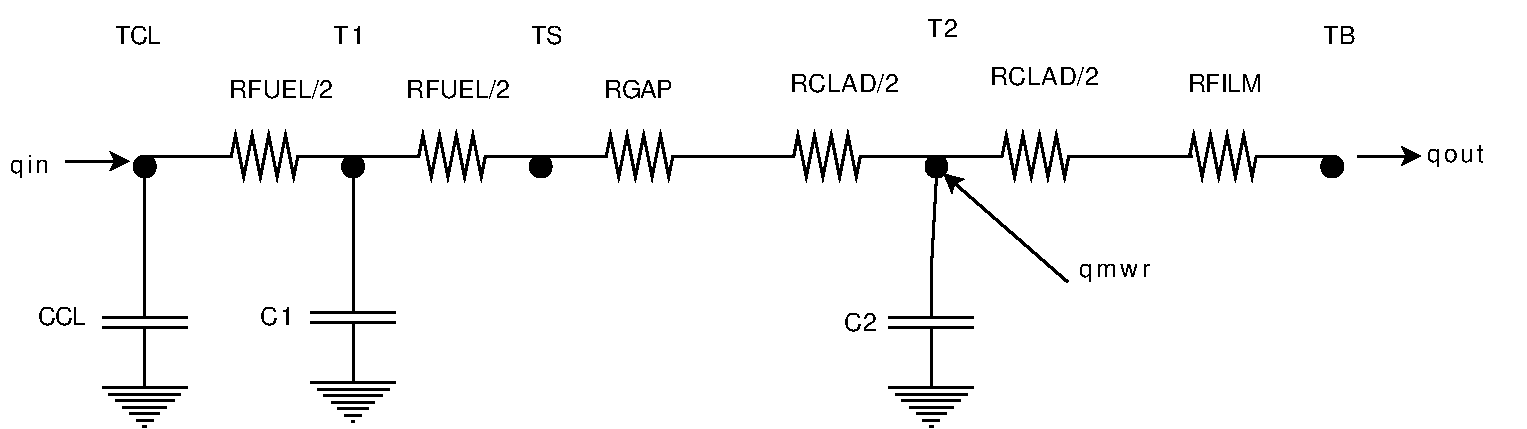
\includegraphics[width=0.9\textwidth]{electricalcircuitanalogue.pdf}
}
\caption{\label{Fig_ECA} Electrical Circuit Analogue}
\end{center}
\end{figure}
~\newline
~\newline

\noindent
\begin{minipage}{\textwidth}
\begin{tabular}{| p{\colAwidth} | p{\colBwidth}|}
\hline
\rowcolor[gray]{0.9}
Number& IM\refstepcounter{instnum}\theinstnum \label{rcat}\\
\hline
Label&Rate of change of average fuel temperature\\
\hline
Equation&$C_1 \frac{dT_1}{dt} = q'_N -\frac{T_1 -T_2}{R_1}$\\
\hline
Description&$T_{1}$ is the average fuel temperature \\
&$T_{2}$ is the average clad temperature \\
&$R_1$ is the effective resistance between average fuel and average clad temperatures \\
&$C_1$ is the thermal capacitance of the fuel \\

\hline
 Sources& \cite[page 6]{FPManual}; \\
\hline
\end{tabular}
\end{minipage}\\
~\newline

\begin{bf}
Derivation of Rate of change of average fuel temperature:
\end{bf}

~\newline
\noindent
To find the rate of change of average fuel temperature, we use
\dref{TRCE}. Consider $c_{p,1}$ as the specific heat evaluated at $T_1$,
$\rho_1$ as the density of the fuel and $A_f$ as area of fuelpellet which is
given as, 

\begin{equation}
A_f=\pi r_f^2 \label{a_f}
\end{equation}

Now substituting $c_{p,1}$, $\rho_1$ and Equation~\ref{a_f} in  Equation~\ref{eq:TAV} gives,

\begin{equation}
\rho_1 c_{p,1} \pi r_f^2 \frac{dT_1}{dt} = q_{\mathrm{in}}-q_{\mathrm{out}}+q_g \label{eq:IMT1t}
\end{equation}

From \ddref{ThermCapTerms} the capacitance term $C_1$ is given as,

\begin{equation}
C_1  = \pi r_f^2 c_{p,1}\rho_1 \label{c_1}
\end{equation}

Rewriting Equation~\ref{eq:IMT1t} and substituting Equation~\ref{c_1} in Equation~\ref{eq:IMT1t} gives

\begin{equation}
C_1 \frac{dT_1}{dt} = q_{\mathrm{in}}-q_{\mathrm{out}}+q_g \label{eq:IMT1}
\end{equation}

The amount of $q_{\text{in}}$  is zero at $T_1$. That is,
\begin{equation}
q_{\text{in}}=0 \label{qin1}
\end{equation}

The value for $q_{\text{out}}$ is given by the flux between $T_1$ and $T_2$.
From the Figure~\ref{Fig_ECA},

\begin{equation}
q_{\text{out}}=\frac{T_1-T_2}{R_1}, \label{qout1}
\end{equation}

where $T_2$ is the average clad temperature and $R_1$ is the effective thermal
resistance between $T_1$ and $T_2$ as given in \ddref{R1}.
\\

The integral of heat generation is,

\begin{equation}
q_{g}=q'_N \label{qgn1}
\end{equation}

Substituting Equation~\ref{qin1}, Equation~\ref{qout1} and Equation~\ref{qgn1}
in Equation~\ref{eq:IMT1}  and rearranging gives,

\begin{equation}
C_1 \frac{dT_1}{dt} = q'_N -\frac{T_1 -T_2}{R_1}
\end{equation}

~\newline
\noindent
\begin{minipage}{\textwidth}
\begin{tabular}{| p{\colAwidth} | p{\colBwidth}|}
\hline
\rowcolor[gray]{0.9}
Number& IM\refstepcounter{instnum}\theinstnum \label{rcclt}\\
\hline
Label&Rate of change of average clad temperature\\
\hline
Equation&$C_2 \frac{dT_2}{dt} =\frac{T_1 -T_2}{R_1}+q'_{\text{MWR}}-\frac{T_2-T_B}{R_2}$\\
\hline
Description&$T_{1}$ is the average fuel temperature \\
&$T_{2}$ is the average clad temperature \\
&$T_{B}$ is the coolant temperature \\
&$R_1$ is the effective resistance between average fuel and average clad temperatures \\
&$R_2$ is the effective resistance between clad and coolant temperatures \\
&$C_2$ is the thermal capacitance of the clad  \\
&$q_{\text{MWR}}$ is the Metal-Water reaction heat \\
\hline
 Sources& \cite[page 6]{FPManual}; \\
\hline
\end{tabular}
\end{minipage}\\
~\newline

\begin{bf}
Derivation of Rate of change of average clad temperature:
\end{bf}

~\newline
Similar to the rate of change of average fuel temperature, to find the rate of
change of average clad temperature, we use \dref{TRCE}. Consider $c_{p,2}$ as
the specific heat evaluated at $T_2$, $\rho_2$ as the density of the clad and
$A_c$ as area of clad which is given as, 

\begin{equation}
A_c=2\pi r_c \tau_c \label{a_c}
\end{equation}

Now substituting $c_{p,2}$, $\rho_2$ and Equation~\ref{a_c} in
Equation~\ref{eq:TAV} gives,

\begin{equation}
\rho_2 c_{p,2}  2\pi r_c \tau_c \frac{dT_2}{dt} = q_{\mathrm{in}}-q_{\mathrm{out}}+q_g \label{eq:IMT2t}
\end{equation}

From \ddref{ThermCapTerms} the capacitance term $C_2$ is given as,

\begin{equation}
C_2 = 2\pi r_c\tau_c c_{p,2}\rho_2 \label{c_2}
\end{equation}

Rewriting Equation~\ref{eq:IMT2t} and substituting Equation~\ref{c_2} in
Equation~\ref{eq:IMT2t} gives

\begin{equation}
C_2 \frac{dT_2}{dt} = q_{\mathrm{in}}-q_{\mathrm{out}}+q_g \label{eq:IMT2}
\end{equation}

$q_{\text{in}}$ at $T_2$ is the amount of  $q_{\text{out}}$ at $T_1$
(\ref{qout1}). That is,

\begin{equation}
q_{\text{in}}= \frac{T_1-T_2}{R_1}\label{qin2}
\end{equation}

The value for $q_{\text{out}}$ is given by the flux between $T_2$ and $T_B$.
From the Figure~\ref{Fig_ECA},

\begin{equation}
q_{\text{out}}=\frac{T_2-T_B}{R_2}, \label{qout2}
\end{equation}

where $R_2$ is the effective thermal resistance between $T_2$ and $T_B$ as given
in \ddref{R2}.
\\
The integral of heat generation is,

\begin{equation}
q_{g}=q'_{\text{MWR}} \label{qgn2}
\end{equation}

Substituting Equation~\ref{qin2}, Equation~\ref{qout2} and Equation~\ref{qgn2}
in Equation~\ref{eq:IMT2}  and rearranging gives,

\begin{equation}
C_2 \frac{dT_2}{dt} =\frac{T_1 -T_2}{R_1}+q'_{\text{MWR}}-\frac{T_2-T_B}{R_2}
\end{equation}

~\newline
\noindent
\begin{minipage}{\textwidth}
\begin{tabular}{| p{\colAwidth} | p{\colBwidth}|}
\hline
\rowcolor[gray]{0.9}
Number& IM\refstepcounter{instnum}\theinstnum \label{rcct}\\
\hline
Label&Rate of change of centerline temperature\\
\hline
Equation&$C_{\text{CL}} \frac{dT_{\text{CL}}}{dt} = q'_N-\frac{T_{\text{CL}}-T_1}{R_{\text{CL}}}$\\
\hline
Description&$T_{1}$ is the average fuel temperature \\
&$T_{\text{CL}}$ is the centerline temperature \\
&$R_{\text{CL}}$ is the effective resistance t the centerline \\
&$C_{\text{CL}}$ is the thermal capacitance at the centerline \\
&$q'_N$ is the linear element power\\
\hline
 Sources& \cite[page 6]{FPManual}; \\
\hline
\end{tabular}
\end{minipage}\\
~\newline

\begin{bf}
Derivation of Rate of centerline temperature:
\end{bf}

~\newline Similar to the rate of change of average fuel temperature, to find the
rate of change of centerline temperature, we use \dref{TRCE}. Consider $c_{p,3}$
as the specific heat evaluated at $T_{\text{CL}}$, $\rho_1$ as the density of
the fuel and $A_f$ as area of fuel pellet which is given by Equation~\ref{a_f}.
Now substituting $c_{p,3}$, $\rho_1$ and Equation~\ref{a_f} in
Equation~\ref{eq:TAV} gives,

\begin{equation}
\rho_1 c_{p,3} \pi r_f^2 \frac{dT_{\text{CL}}}{dt} = q_{\mathrm{in}}-q_{\mathrm{out}}+q_g \label{eq:IMT3t}
\end{equation}

From \ddref{ThermCapTerms} the capacitance term $C_{\text{CL}}$ is given as,

\begin{equation}
C_{\text{CL}} = \pi r_f^2 c_{p,3}\rho_1 \label{c_3}
\end{equation}

Rewriting Equation~\ref{eq:IMT3t} and substituting Equation~\ref{c_3} in
Equation~\ref{eq:IMT3t} gives

\begin{equation}
C_{\text{CL}} \frac{dT_{\text{CL}}}{dt} = q_{\mathrm{in}}-q_{\mathrm{out}}+q_g \label{eq:IMT3}
\end{equation}

From the Figure~\ref{Fig_ECA}, $q_{\text{in}}$ at $T_{\text{CL}}$ is the linear
element power $q'_N$. That is,

\begin{equation}
q_{\text{in}}=q'_N \label{qin3}
\end{equation}

The value for $q_{\text{out}}$ is given by the flux between $T_{\text{CL}}$ and $T_1$.
From the Figure~\ref{Fig_ECA},

\begin{equation}
q_{\text{out}}=\frac{T_{CL}-T_1}{R_{\text{CL}}}, \label{qout3}
\end{equation}

where $R_{\text{CL}}$ is the effective thermal resistance between
$T_{\text{CL}}$ and $T_1$ as given in \ddref{rcl}.
\\
The integral of heat generation is,

\begin{equation}
q_{g}=0\label{qgn3}
\end{equation}

Substituting Equation~\ref{qin3}, Equation~\ref{qout3} and Equation~\ref{qgn3}
in Equation~\ref{eq:IMT3}  and rearranging gives,

\begin{equation}
C_{\text{CL}} \frac{dT_{\text{CL}}}{dt} = q'_N-\frac{T_{\text{CL}}-T_1}{R_{\text{CL}}}
\end{equation}

~\newline
\noindent
\begin{minipage}{\textwidth}
\begin{tabular}{| p{\colAwidth} | p{\colBwidth}|}
\hline
\rowcolor[gray]{0.9}
Number& IM\refstepcounter{instnum}\theinstnum \label{InitConds}\\
\hline
Label&Initial thermal conditions\\
\hline
Equation&$\frac{dT_1}{dt} =0$ (IM\ref{rcat})\\
&$\frac{dT_2}{dt} =0$ (IM\ref{rcclt})\\
&$k_c =aT_2+b$  (\ddref{kc})\\
&$q'_{\text{MWR}} =0$\\

&$q'_{\text{N,est}}=4\pi \int_{T_S}^{T_{\text{CL,est}}} kdT=q'_N$\\
\hline
Description & 
The initial values that are needed to start the simulation are calculated using
the above conditions.
\\
&$T_{1}$ is the average fuel temperature \\
&$T_{2}$ is the average clad temperature \\
&$T_{S}$ is the surface temperature \\
&$T_{\text{CL,est}}$ is the estimate of centerline temperature \\
&$k_c$ is the clad conductivity  which is given by \ddref{kc}\\

&$a,b$ are constants with their values given by Table~\tbref{k_c}\\
&$q'_{\text{MWR}}$ is the Metal-Water reaction heat\\
&$q'_{\text{N,est}}$ is the estimate of linear element power\\
&$k$ is the fuel conductivity\\

\hline
 Sources& \cite[page 6]{FPManual}; \\
\hline
\end{tabular}
\end{minipage}\\

~\newline
\noindent
\begin{minipage}{\textwidth}
\begin{tabular}{| p{\colAwidth} | p{\colBwidth}|}
\hline
\rowcolor[gray]{0.9}
Number& IM\refstepcounter{instnum}\theinstnum \label{PointNeutronKinetics}\\
\hline
Label&Point neutron kinetics\\
\hline
Equation&$\dot{N} = [\frac{\rho-\beta}{l^*}]  N +\Sigma_{i=1}^6 \lambda_i c_i$\\
&$\dot{c_i}= -\lambda_i c_i + (\frac{\beta_i}{l^*}) N$\\
\hline
Description&$N$ is the neutron flux\\
&$\rho$ is the reactivity\\
&$\beta_i$ is the fraction associated with the $i^{th}$ group of delayed neutron
precursors\\
&$\beta$ is total delayed neutron fraction\\
&$l^*$ is the prompt generation time(s)\\
&$\lambda_i$ is the decay constant associated with the $i^{th}$ group of delayed
neutron precursors ($s^{-1}$)\\
&$c_i$ is the delayed neutron precursor for the $i^{th}$ group\\
& To make the relative distribution of the neutrons uniform, the space effects
on the kinetics equations are to be eliminated. Hence taking \aref{A_stk} into
consideration, i.e considering only time effects, the space-time kinetics
equations of \tref{T_STK} is reduced to the point kinetics equations. If the
reactivity transient is given as input, the transient neutron flux is obtained
by solving the point kinetics equations.
\\
\hline
 Sources& \cite[page 6]{FPManual}; \\
\hline
\end{tabular}
\end{minipage}\\

~\newline
\noindent
\begin{minipage}{\textwidth}
\begin{tabular}{| p{\colAwidth} | p{\colBwidth}|}
\hline
\rowcolor[gray]{0.9}
Number& IM\refstepcounter{instnum}\theinstnum \label{DecayHeatEquation}\\
\hline
Label&Decay Heat Equations\\
\hline
Equation&$q'_{\text{NFRAC}}= (1 -\gamma)  N + \Sigma_{i=1}^3\lambda_{h,i} W_i$\\
&$\dot{W_i}=-\lambda_{h,i} W_i + \gamma_i N$\\
\hline
Description&$N$ is the neutron flux\\
&$q'_{\text{NFRAC}}$ is the relative fuel power\\
&$\gamma_i$ is the power fraction associated with the $i^{th}$ decay heat group\\
&$\lambda_{h,i}$ is the decay constant associated with the $i^{th}$ decay heat group $(s^{-1})$\\
&$\gamma$ is the total delayed power fraction\\
&$W_i$ is the relative decay heat amplitude for the $i^{th}$ group\\
& The decay equations are used in generating fuel power. The total fuel power is
a summation of a prompt neutronic power component (the prompt fission power) and
three delayed decay heat components due to fission product decay. If the neutron
flux transient is given as input or from the point kinetics routine, the
transient fuel power is obtained by solving the decay heat equations. 
\\
\hline
 Sources& \cite[page 6]{FPManual}; \\
\hline
\end{tabular}
\end{minipage}\\

\subsubsection{Data Constraints}    

This section is to clarify the environmental and system limitations imposed on
admissible data. It gives the system constraints on the data to validate the
models identified in the section ``Instance Models''. These constraints are
listed in the table below. The column physical constraints gives the physical
limitations on the range of the values that can be taken by the variable and are
given by the domain expert while the column system constraints gives the system
limitations on the range of values that can be taken by the variable and are
given by the developer.  In this case no system constraints are imposed, so this
column is not included.

\noindent
%\begin{table}
\begin{longtable}{| p{\colCwidth} | p{\colCwidth} | p{\colDwidth}| p{\colAwidth}|
    p{\colFwidth}|p{\colCwidth}|}
\hline
\rowcolor[gray]{0.9}
Variable & Type & Unit & Physical Constraints & Typical value & Property\\
\hline
$\lambda_{h,1}$&Real&$\text{s}^{-1}$&$ -\infty <\lambda_{h,1}<\infty $&0.10368&IN\\
\hline
$\lambda_{h,2}$&Real&$\text{s}^{-1}$&$ -\infty <\lambda_{h,2}<\infty $&0.000142&IN\\
\hline
$\lambda_{h,3}$&Real&$\text{s}^{-1}$&$ -\infty <\lambda_{h,3}<\infty $&0.00476&IN\\
\hline
$\gamma_1$&Real&-&$-\infty <\gamma_1<\infty$&0.0226&IN\\
\hline
$\gamma_2$&Real&-&$-\infty <\gamma_2<\infty$&0.02311&IN\\
\hline
$\gamma_3$&Real&-&$-\infty <\gamma_3<\infty$&0.02078&IN\\
\hline
$N$&Real&&to be discussed&&IN-OUT\\
\hline
$\rho_1$&Real&$\frac{\text{kg}}{\text{m}^3}$&$-\infty< \rho_1<\infty$&10600&IN\\
\hline
$\rho_2$&Real&$\frac{\text{kg}}{\text{m}^3}$&$-\infty< \rho_2<\infty$&6570&IN\\
\hline
$\rho$ (reactivity)&Real&&to be discussed&0&IN-OUT\\
\hline
$\tau_c$&Real&$\text{m}$&$-\infty< \tau_c<\infty$&0.00042&IN\\
\hline
$\tau_g$&Real&$\text{m}$&$-\infty< \tau_g<\infty$&0.00004&IN\\
\hline
$\tau_A$&Real&-&$-\infty< \tau_A<\infty$&0.015&IN\\
\hline
$\Delta T$&Real&$\text{s}$&$0<\Delta T\leq$ 0.0001&0.01&IN\\
\hline
$f$&Real&-&$-\infty< f<\infty$&1.0&IN\\
\hline
$l^*$&Real&$\text{s}$&$-\infty< l^* <\infty$&0.893$\times 10^{-3}$&IN\\
\hline
$\beta_1$&Real&-&$-\infty < \beta_1<\infty$&1.769$\times 10^{-4}$&IN\\
\hline
$\beta_2$&Real&-&$-\infty < \beta_2<\infty$&11.498$\times 10^{-4}$&IN\\
\hline
$\beta_3$&Real&-&$-\infty < \beta_3<\infty$&10.191$\times 10^{-4}$&IN\\
\hline
$\beta_4$&Real&-&$-\infty < \beta_4<\infty$&21.057$\times 10^{-4}$&IN\\
\hline
$\beta_5$&Real&-&$-\infty < \beta_5 <\infty$&7.726$\times 10^{-4}$&IN\\
\hline
$\beta_6$&Real&-&$-\infty < \beta_6 <\infty$&1.962$\times 10^{-4}$&IN\\
\hline
$\beta_7$&Real&-&$-\infty < \beta_7 <\infty$&1.61$\times 10^{-7}$&IN\\
\hline
$\beta_8$&Real&-&$-\infty < \beta_8 <\infty$&3.23$\times 10^{-7}$&IN\\
\hline
$\beta_9$&Real&-&$-\infty < \beta_9<\infty$&1.03$\times 10^{-6}$&IN\\
\hline
$\beta_{10}$&Real&-&$-\infty < \beta_{10}<\infty$&7.48$\times 10^{-6}$&IN\\
\hline
$\beta_{11}$&Real&-&$-\infty < \beta_{11}<\infty$&6.61$\times 10^{-6}$&IN\\
\hline
$\beta_{12}$&Real&-&$-\infty < \beta_{12}<\infty$&1.080$\times 10^{-5}$&IN\\
\hline
$\beta_{13}$&Real&-&$-\infty < \beta_{13}<\infty$&2.240$\times 10^{-5}$&IN\\
\hline
$\beta_{14}$&Real&-&$-\infty < \beta_{14}<\infty$&6.52$\times 10^{-5}$&IN\\
\hline
$\beta_{15}$&Real&-&$-\infty < \beta_{15}<\infty$&2.080$\times 10^{-4}$&IN\\
\hline
$\lambda_1$&Real&$\text{s}^{-1}$&$-\infty <\lambda_1 <\infty$&12.778$\times 10^{-3}$&IN\\
\hline
$\lambda_2$&Real&$\text{s}^{-1}$&$-\infty <\lambda_2 <\infty$&31.535$\times 10^{-3}$&IN\\
\hline
$\lambda_3$&Real&$\text{s}^{-1}$&$-\infty <\lambda_3 <\infty$&122.197$\times 10^{-3}$&IN\\
\hline
$\lambda_4$&Real&$\text{s}^{-1}$&$-\infty <\lambda_4 <\infty$&32.282$\times 10^{-2}$&IN\\
\hline
$\lambda_5$&Real&$\text{s}^{-1}$&$-\infty <\lambda_5 <\infty$&1389.289$\times 10^{-3}$&IN\\
\hline
$\lambda_6$&Real&$\text{s}^{-1}$&$-\infty <\lambda_6 <\infty$&3778.336$\times 10^{-3}$&IN\\
\hline
$\lambda_7$&Real&$\text{s}^{-1}$&$-\infty <\lambda_7 <\infty$&6.26$\times 10^{-7}$&IN\\
\hline
$\lambda_8$&Real&$\text{s}^{-1}$&$-\infty <\lambda_8 <\infty$&3.63$\times 10^{-6}$&IN\\
\hline
$\lambda_9$&Real&$\text{s}^{-1}$&$-\infty <\lambda_9 <\infty$&4.37$\times 10^{-5}$&IN\\
\hline
$\lambda_{10}$&Real&$\text{s}^{-1}$&$-\infty <\lambda_{10} <\infty$&0.117$\times 10^{-3}$&IN\\
\hline
$\lambda_{11}$&Real&$\text{s}^{-1}$&$-\infty <\lambda_{11} <\infty$&0.428$\times 10^{-3}$&IN\\
\hline
$\lambda_{12}$&Real&$\text{s}^{-1}$&$-\infty <\lambda_{12} <\infty$&0.150$\times 10^{-2}$&IN\\
\hline
$\lambda_{13}$&Real&$\text{s}^{-1}$&$-\infty <\lambda_{13} <\infty$&0.481$\times 10^{-2}$&IN\\
\hline
$\lambda_{14}$&Real&$\text{s}^{-1}$&$-\infty <\lambda_{14}<\infty$&0.169*$10^{-1}$&IN\\
\hline
$\lambda_{15}$&Real&$\text{s}^{-1}$&$-\infty <\lambda_{15} <\infty$&0.277&IN\\
\hline
$q'_{N,\text{max}}$&Real&$\frac{\text{kW}}{\text{m}}$&$35\leq q'_{N,\text{max}} \leq 65$&62.9540&IN\\
\hline
$h_b$&Real&$\mathrm{\frac{kW}{m^{2o}C}}$&$-\infty <h_b<\infty$&50&IN\\
\hline
$h_p$&Real&$\mathrm{\frac{kW}{m^{2o}C}}$&$-\infty <h_p<\infty$&10&IN\\
\hline
$T_B$&Real&$^oC$&$-\infty <T_B<\infty$&305.0&IN\\
\hline
$r_f$&Real&$\text{m}$&$-\infty <r_f<\infty$&0.00612&IN\\
\hline
$p_{\text{dry}}$&Real&$fp$&$-\infty <p_{\text{dry}}<\infty$&1.176&IN\\
\hline
$h_{\text{dry}}$&Real&$\mathrm{\frac{kW}{m^{2o}C}}$&$-\infty<h_{\text{dry}}<\infty$&2.0&IN\\
\hline
\end{longtable}
%\caption{Table showing Data Constraints (no System Constraints are imposed)}
%\end{table}

\subsubsection{System Behaviour}    

This section gives a detailed description of the  system's functionalities based
on the information  in the sections``Data Constraints'' and ``Instance
Models''. It formally specifies the flow of  processing the data. That is, from
getting the input, applying the models and producing the output. The responses
to undesired situations such as the errors that are to be generated if the data
constraints are not satisfied are also stated. The contents of this section are
used in design and testing.

~\newline

\noindent Step 1: Read data from the Input file

\begin{enumerate}

\item Read the driving transient data
  \\
  \indent \ If the driving transient is reactivity, then
  \\
  \indent \ \ Read the reactivity transient data ($\rho(t)$)
  \\
  \indent
  \ Else if the driving transient is neutron flux, then\\
  \indent \ \ Read the Neutron flux transient data ($N(t)$)
  \\
  \indent
  \ Else \\
  \indent \ \ Read Fuel power transient data ($q'_{\text{NFRAC}}(t)$)

\item Read the inputs\\
  \indent \ Read the inputs $\Delta t,\tau_c,\tau_g,h_g,h_b,\rho 1,\rho2,r_i$
  \\
  \indent \ If the driving transient is $\rho(t)$, then ~\newline
  \indent \ \  Read $l^*$, $\beta_i$, $\gamma_i$ \\
  \indent \  If the driving transient is $\rho(t)$ or $N(t)$, then\\
  \indent \ \ Read the inputs $\gamma_{h,i}$, $\lambda_i$
\end{enumerate}

\noindent Step 2: Process/Output:
~\newline 
\indent \ For each time step,

\begin{enumerate}
\item If the driving transient is $\rho(t)$, then
  \\
  \indent \ Determine reactivity based on current time\\
  \indent Else if the driving transient is $N(t)$, then\\
  \indent \ Determine neutron flux based on current time\\
  \indent Else if the driving transient is $q'_{\text{NFRAC}}(t)$, then\\
  \indent \ Determine fuel power based on current time
\item
  If the driving transient is $\rho(t)$, then
  \begin{enumerate}
  \item Generate the Neutron flux solving Point kinetics equations from
    \iref{PointNeutronKinetics}
  \item Output Neutron flux ($N$)
  \end{enumerate}

\indent Else if the driving transient is $\rho(t)$ or $N(t)$, then

\begin{enumerate} 
\item Generate the relative fuel power by solving Decay heat equations from
  \iref{DecayHeatEquation}
\item Output the relative fuelpower ($q'_{\text{NFRAC}}$)
\end{enumerate}

\indent Else if the driving transient is $\rho(t)$ or $N(t)$ or
$q'_{\text{NFRAC}}(t)$, then

\begin{enumerate}
\item Change the relative fuel power to linear element power using
  \ddref{LEP} \label{s2}
\item Use the linear element power to determine average fuel temperature,
  average clad temperature and centerline temperature by solving \iref{rcat},
  \iref{rcct} ,\iref{rcclt} respectively
\item Output  $T_1,T_2,T_{\text{CL}}$
\item Use $T_1$, $T_2$ to determine Surface temperature ($T_S$) by solving
  \ddref{$T_S$}
\item Output  $T_S$
\item Using the generated $T_1$, find the fuel stored energy ($\Delta H(T_1)$)
  using \ddref{FuelStoredEnergy} and the power to the coolant
  ($q'_{\text{out}})$ using \ddref{qout}
\item Find the fuel power ($f_p$) using \ddref{IntegFuelPow}\\
  \indent If Metal water reaction's calculations are desired, then
\item  Read $p_{\text{dry}}$, $h_{\text{dry}}$, $\delta_{\text{ox}}$
\item Calculate the Metal water reaction heat using \ddref{MetalWatReact} and
  \ddref{qmwri}
\end{enumerate}
\end{enumerate}

~\newline
\subsection{Nonfunctional Requirements}

This section specifies system requirements that consider the quality and
behaviour of the system as a whole. It provides different specifications for the
system, so that it is found acceptable and pleasant to use.These include:
Accuracy/performance requirements, maintainability requirements.

\subsubsection{Accuracy}

The relative error between FP code and HOTSPOT code for the test cases specified
in the FP Engineer's manual should not be more than 0.05 ~\newline

\subsubsection{Maintainability}

The effort put in maintaining the product should be less than 1/4th of the
amount of efforts put in building, developing the software.  ~\newline

\subsubsection{Solution Validation Strategies}

This section establishes the strategies for validating the software product, and
the specific tests to be performed to assert it complies with the requirements
specification defined in the previous section. To validate the solution produced
by the software,

1. Results of the FP code are compared with those of the HOTSPOT code for a test
transient.

\begin{itemize}

\item An idealized transient involving severe overpower, combined with step
  changes in coolant temperature and an order of magnitude reduction in
  convective heat transfer to coolant, should be run with both codes.
\item Runs are to performed both with and without average flux depression
  factor.
\end{itemize}

\section{Other System Issues}

This section provides additional information ``on the side'' about FP

\subsection{Open Issues}

None present

\subsection{ Off-the-Shelf Solutions}
   
None present

\subsection{ Waiting Room}

None Present

\section{Traceability Matrix}

The purpose of this matrix is to provide an easy reference on what has to be
additionally modified if a certain component is changed. Every time a component
is changed, then the items in the column of that component which cross into an
``X'' should be modified as well.
\\
~\newline

NOTE: Traceability Matrix of a subset of the components is developed to keep the
matrix fit in one page. The references between the other items would be
documented in a similar manner. Building a tool to automatically generate the
graphical representation of the matrix by scanning the labels and references can
be a future work.
\\
~\newline

\noindent
\begin{table}
\begin{minipage}{\textwidth}
  \begin{tabular}{| p{7.5mm} |
      p{5mm} | p{5mm} | p{5mm} | p{5mm} |
      p{5mm} | p{5mm} | p{7mm} | p{7mm} |
      p{7mm} | p{7mm} | p{7mm} | p{7mm} |
      p{7mm} | p{7mm} | p{7mm}|}

    \hline
    &T1 &T2 &T3 &A1 &A2 &A3 &GD1&GD2 &GD3 &GD4&GD5&DD6&DD7&DD8&DD9\\
    \hline
    GD1&&&&&&&&&&&&&&&\\
    \hline
    GD2&&&&X&X&&X&&&&&&&&\\
    \hline
    GD3&&&&&&&&&&&&&&&\\
    \hline
    GD4&X&&&&&&&X&&&&&&&\\
    \hline
    GD5&&X&&&&&&&&&&&&&\\
    \hline
    GD6&&X&&&&&&&&&&&&&\\
    \hline
    DD1&&&&&&&&&&&&&&&\\
    \hline
    DD2&&&&&&&&&&&&&&&\\
    \hline
    DD3&&&&&&&&&&&&&&&\\
    \hline
    DD4&&&&&&&&&&&&&&&\\
    \hline
    DD5&&&&&&&&&&&&&&&\\
    \hline
    DD6&&&&&&&&X&X&&&&&&\\
    \hline
    DD7&&&&&&&&&X&&&&&&\\
    \hline
    DD8&&&&&&&&&X&&X&&&&\\
    \hline
    DD9&&&&&&&&&X&&X&&&&\\
    \hline
    DD10&&&&&&&&&X&&&&&&\\
    \hline
    DD11&&&&&&&&&&&&X&&&\\
    \hline
    DD12&&&&&&&&&X&&&&&&\\
    \hline
    DD13&&&&&&&&X&X&&&&&&\\
    \hline
    DD14&&&&&&&&&&&&&&&\\
    \hline
    DD15&&&&&&&&&&&&&&&\\
    \hline
    DD16&&&&&&&&&&&&&&&\\
    \hline
    DD17&&&&&&&&&&&&&&&\\
    \hline
    Dd18&&&&&&&&&&&&&X&&X\\
    \hline
    DD19&&&&&&&&&&&&&X&X&\\
    \hline
    DD20&&&&&&&&&&&&&&&\\
    \hline
    DD21&&&&&&&&&&&&&&&\\
    \hline
    DD22&&&&&&&&&&&&&&&\\
    \hline
    DD23&&&&&&X&&&X&&&&&&\\
    \hline
    DD24&&&&&&&&&&&&&&&\\
    \hline
    DD25&&&&&&&&&&&&&&&\\
    \hline
    DD26&&&&&&&&&&&&&&&\\
    \hline
    DD27&&&&&&&&&X&&&&&&\\
    \hline
    DD28&&&&&&&&&&&&&&&X\\
    \hline
    IM1&&&&&&&&&&X&&&&&\\
    \hline
    IM2&&&&&&&&&&X&&&&&\\
    \hline
    IM3&&&&&&&&&&X&&&&&\\
    \hline
    IM5&&&X&&&&&&&&&&&&\\
    \hline
\end{tabular}
\caption{Traceability Matrix Showing the Connections Between Items of Different Sections}
\end{minipage}
\end{table}
~\newline
~\newline

\section{Auxillary Constants}

\noindent

\begin{minipage}{\textwidth}

\begin{tabular}{| p{\colEwidth}|}
  \hline
  \bf {TB\refstepcounter{tablenum}\thetablenum \label{mwr}} Metal Water Reaction\\
  \hline
\end{tabular}

\begin{tabular}{| p{\colCwidth} | p{\colAwidth}| p{\colAwidth} | p{\colAwidth}|}
  \hline
  Constant & Value &Constraint &Units \\
  \hline
  A  
  &$6.48 \times 10^{-8}$ &$ T_2 \leq  1580^oC$ &- \\
  \cline{2-4}

  &$1.0 \times 10^{-6}$   & $T_2 > 1580^oC$ &- \\
  \hline
  B/R  &13586.0  &$ T_2 \leq  1580^oC$ &-\\
  \cline{2-4}
  &16014.0  & $T_2 > 1580^oC$ &- \\
  \hline
  $q_r$ &6500.0 &- &$\mathrm{\frac{kJ}{kg}}$ \\
  \hline
\end{tabular}
\end{minipage}\\
~\newline 

\noindent

\begin{minipage}{\textwidth}
\begin{tabular}{| p{\colEwidth}|}
\hline
\bf {TB\refstepcounter{tablenum}\thetablenum \label{k_c}} Clad Conductivity\\

\hline
\end{tabular}
\begin{tabular}{| p{\colCwidth} | p{\colAwidth}| p{\colAwidth} | p{\colAwidth}|}
  \hline
  Constant & Value &Constraint &Units \\
  \hline
  a  &$1.43 \times 10^{-5}$  & $T_2 \leq1000^oC$ &- \\
  \cline{2-4}
  &$2.73 \times 10^{-5}$ &$T_2 > 1000^oC$ &- \\
  \hline
  b  &$1.17  \times 10^{-2} $ &$T_2 \leq 1000^oC$ &-\\
  \cline{2-4}
  &$-1.27 \times 10^{-3}$ &$T_2 > 1000^oC$ &- \\
  \hline
\end{tabular}
\end{minipage}\\
~\newline

\begin{minipage}{\textwidth}

\begin{tabular}{| p{\colEwidth}|}
  \hline
  \bf {TB\refstepcounter{tablenum}\thetablenum \label{kav}} Coefficients for polynomial $K_{\text{AV}}$\\
  \hline
\end{tabular}

\begin{tabular}{| p{\colFwidth} | p{\colFwidth}|p{\colAwidth}|p{\colFwidth}|}
  \hline
  Coefficient & Value &Constraint &Units  \\
  \hline
  $x_0$ & &&\\
  \hline
  $x_1$ &&&\\
  \hline
\end{tabular}

\end{minipage}\\
~\newline


\begin{minipage}{\textwidth}

\begin{tabular}{| p{\colEwidth}|}
  \hline
  \bf {TB\refstepcounter{tablenum}\thetablenum \label{cp}} Coefficients for polynomial $c_{p,1}$\\
  \hline
\end{tabular}

\begin{tabular}{| p{\colFwidth} | p{\colFwidth}|p{\colAwidth}|p{\colFwidth}|}
  \hline
  Coefficient & Value &Constraint &Units  \\
  \hline
  $y_0$ & &&\\
  \hline
  $y_1$ &&&\\
  \hline
  $y_2$ &&&\\
  \hline
\end{tabular}

\end{minipage}\\
~\newline

\begin{minipage}{\textwidth}

\begin{tabular}{| p{\colEwidth}|}
  \hline
  \bf {TB\refstepcounter{tablenum}\thetablenum \label{fse}} Fuel Stored Energy\\
  \hline
\end{tabular}

\begin{tabular}{| p{\colCwidth} | p{\colAwidth}| p{\colAwidth} | p{\colAwidth}|}
  \hline
  Constant & Value &Constraint &Units \\
  \hline
  $K_0$  &15.496 &- &-\\
  \hline
  $K_1$ &19.145 &- &$\mathrm{\frac{cal}{mole K}}$  \\
  \hline
  $K_2$ & $7.84733\times 10^{-4} $&- & $\mathrm{\frac{cal}{mole K^2}}$\\
  \hline
  $K_3$ & $5.64373 \times 10^6$ &- &$\mathrm{\frac{cal}{mole}}$\\
  \hline
  $\theta$ &535.285 &- &$\mathrm{K}$ \\
  \hline
  $E_D/R$ & $1.8971\times 10^4$ &- &$\mathrm{K}$ \\
  \hline
\end{tabular}
\end{minipage}\\

\chapter{LP Manual}

\M{1}
\section{Overview}


Given relative fuel power ($q'_{\mathrm{NFRAC}}$) as input, the
function {\PB{\\{fuel\_temp\_}}}
calculates the following:
\begin{enumerate}
\item Average fuel temperature ($T_1$),
\item Average Clad temperature ($T_2$),
\item Centerline temperature ($\tclad$),
\item Surface temperature ($T_S$), and
\item Stored fuel energy $(\Delta H(T_{\text{abs}}))$.
\item Integrated fuel power $(f_p)$.
\item Power to the coolant $(q'_{\text{out}})$.
\item Metal water reaction heat $(q'_{\text{MWR}})$.
\end{enumerate}


This function uses
\begin{itemize}
\item the material properties of the clad and fuelpellet

\item lumped parameter methods and

\item initial conditions
\end{itemize}
It solves the ODE’s from the SRS given by IM\ref{L-rcat}, IM\ref{L-rcct} and
IM\ref{L-rcclt} with the initial conditions defined in IM\ref{L-InitConds},
which are summarized below:
\begin{align}
C_1 \frac{dT_{1}}{dt} &= q'_N-\frac{T_{1}-T_2}{R_1} \label{eq:T_1}\\
C_2 \frac{dT_{2}}{dt} &=\frac{T_1-T_2}{R_1}+ q'_{\mathrm{MWR}}-%
\frac{T_2-T_B}{R_2}
\label{eq:T_2}\\
C_{\text{CL}} \frac{d \tclad}{dt} &= q'_N-\frac{T_{\mathrm{CL}}-T_1}{R_{%
\text{CL}}}
\label{eq:T_3}
\end{align}
%
where
\begin{itemize}
\item $T_B$ is the coolant temperature
\item $q'_{N}$ is the linear element power  ($\text{{kW}/{m}}$)
\item
$q'_{\mathrm{MWR}}$ is metal-water reaction heat  ($\text{{kW}/{m}}$)
\item $C_1$ is the thermal capacitance of the
fuel ($\text{{kWs}/{(m\degree C)}}$)
\item $C_2$ is the thermal capacitance of the clad  ($\text{{kWs}/{(m\degree
C)}}$)
\item $C_{\text{CL}}$ is the thermal capacitance at the centerline
($\text{{kWs}/{(m\degree C)}}$)
\item $R_1$ is the effective thermal resistance between
$T_1$ and $T_2$ $(\text{{m\degree C}/{kW}})$
\item $R_2$ is the effective thermal resistance between coolant and half of the
clad $(\text{{m\degree C}/kW})$
\item $R_{\text{CL}}$ is the thermal resistance between $T_{\text{CL}}$ and
$T_1$
$(\text{{m\degree C}/{kW}})$
\item $t$ is time
\end{itemize}

\section{Numerical Algorithm}
~\newline
Equations~\ref{eq:T_1}--\ref{eq:T_3} are of the form:
\begin{equation}
\frac{dx}{dt}=a(x)x+b(x)u(x,t) \label{eq:DE},
\end{equation}
where $x$ is the variable under consideration. Taking the Laplace
transform of Equation~\ref{eq:DE},
\begin{equation}
x(s)=\frac{x_0}{s-a}+\frac{bu}{s(s-a)} \label{eq:LT}
\end{equation}
with $x_0$ being $x(t_0)$.
To obtain the closed form solution, $a(x)$, $b(x)$ and $u(x,t)$ are assumed
to be constant in the interval [$t$, $t+\Delta t$].
The solution to the above ODE is found by taking the inverse Laplace transform
of
Equation~\ref{eq:LT}
\begin{equation}
x(t)=x_oe^{-at}+bu\int^t_0e^{-at}dt
\end{equation}
Denoting an approximation of $x(t_k)$ at $t_k$ by $x_{k}$ and denoting
$\Delta t = t_{k+1}-t_k$, $k\ge 0$, we have:
\begin{equation}
x_{k+1}=x_ke^{-a_k\Delta t} + (1-e^{-a_k\Delta t})%
\frac{-b(x_k)u(x_k,t_k)}{a(x_k)}
\label{eq:ODE}
\end{equation}
The following table summarizes the values of $a(x)$, $b(x)$ and $u(x,t)$ for
Equations
\ref{eq:T_1}, \ref{eq:T_2} and \ref{eq:T_3}:
\noindent
\begin{table}[H]
\centering
\begin{tabular}{c c c c c} \hline
Equation& $x$& $a(x)$& $b(x)$& $u(x,t)$ \\
\hline
\ref{eq:T_1}& $T_1$&$-\frac{1}{R_1 C_1 }$&$\frac{T_2+q'_{N}R_1}{ R_1 C_1 }$&$1$
\\
\hline
\ref{eq:T_2}&$T_2$&$-\frac{(R_1+ R_2) }{R_1 R_2 C_2 }$&$\frac{T_1 R_2+q'_{%
\mathrm{MWR}}R_1 R_2+
T_B R_1}{R_1 R_2 C_2 }$&$1$\\
\hline
\ref{eq:T_3}&$T_{\text{CL}}$&$-\frac{1}{R_3 C_{\text{CL}}}$&$\frac{T_1+q'_N
R_3}
{R_3C_{\text{CL}}}
$&$1$\\
\hline \end{tabular}
\caption{Table of functions for ODEs representing different instance models}
\end{table} \label{Tab:1}

\section{Algorithm}

{${\bf fuel\_temp\_}(\Delta t, q_{\text{NFRAC},k},q'_{N_{\text{max}}},r_f, f, %
\rho_1,
\rho_2, h_{ib}, h_p, \tau_g, \tau_c, T_{b}, p_{\text{dry}}, h_{\text{dry}},
\text{time}, init\_flag,
MW\_flag,n,\\ h_{b,k},q'_{N,k}, k_{c,k}, k_{\text{AV},k}, q'_{\text{MWR},k},
f_{p,k}, T_{1,k}, T_{2,k}, T_{\text{CL},k}, T_{S,k}, h_{c,k}, h_{g,k}, C_{1,k},
C_{2,k},
C_{\text{CL},k}, c_{p,1,k}, c_{p,2,k}, c_{p,3,k}, \Delta H(T_{\text{abs},k}),\\
\delta_{\text{ox},k}, R_{\text{ox},k}, q'_{\text{out},k}, q'_{\text{MWRI},k})$
\begin{enumerate}
\item Initialization section ($*init\_flag==1$):
\begin{itemize}
\item Input: $\Delta t$, $q_{\text{NFRAC},0}$, $q'_{N_{\text{max}}}$,$r_f$,
$f$,
$\rho_1$, $\rho_2$,  $h_{ib}$, $h_p$, $\tau_g$, $\tau_c$, $T_{b}$, \PB{\\{init%
\_flag}}.

\item At $t_0$ compute $y_{0}$

\item Output: $y_{0}$,

\end{itemize}
where $y_{0}= \{ h_{b},q'_{N}, k_{c}, k_{\text{AV}},q'_{\text{MWR}},
f_{p},T_{1}, T_{2}, T_{\text{CL}}, T_{S}, C_{1}, C_{2}, C_{\text{CL}},
c_{p,1}, c_{p,2}, c_{p,3}, h_{c}, h_{g},\\ \Delta H(T_{\text{abs}}),
\delta_{\text{ox}}, R_{\text{ox}}, q'_{\text{out}}, q'_{\text{MWRI}}\}$. \\
All elements of the set $y_0$ are evaluated at the
$0^{\text{th}}$ time step.

\item Dynamic section ($*init\_flag==0$):
\fi

\M{2}At $t_{k+1}$, $k\ge 0$,
\begin{itemize}

\item Input:$\Delta t$, $q_{\text{NFRAC},k+1}$, $q'_{N_{\text{max}}}$,$r_f$,
$f$,
$\rho_1$, $\rho_2$,  $h_{ib}$, $h_p$, $\tau_g$, $\tau_c$, $T_{b}$, $p_{%
\text{dry}}$,
$h_{\text{dry}}$, $\text{time}$, \PB{\\{init\_flag}}, \PB{\\{MW\_flag}}, $n$,
$y_k$.
\item compute $y_{k+1}$, update $n$ when necessary.
\item Output: $y_{k+1}$, $n$,
\end{itemize}
where $y_{k+1}= \{h_b, q'_{N}, k_{c}, k_{\text{AV}},q'_{\text{MWR}},
f_{p},T_{1}, T_{2}, T_{\text{CL}}, T_{S}, C_{1}, C_{2}, C_{\text{CL}},
c_{p,1}, c_{p,2}, c_{p,3}, h_{c}, h_{g}, \\ \Delta H(T_{\text{abs}}),
\delta_{\text{ox}}, R_{\text{ox}}, q'_{\text{out}},q'_{\text{MWRI}}\}$.\\
All elements of the set $y_{k+1}$ are evaluated at the $k+1^{\text{th}}$ time
step.
\end{enumerate}
~\newline

\section{Overall function}

\Y\B\4\X2:fuel temp function\X${}\E{}$\6
\&{void} \\{calpro\_}(\&{float} ${}{*}\|t,\39{}$\&{int} ${}{*}\|i,\39{}$\&{int}
${}{*}\\{iflag},\39{}$\&{float} ${}{*}\\{prpval},\39{}$\&{int} ${}{*}%
\\{icnt});{}$\6
\&{void} \\{dryout\_}(\&{float} ${}{*}\\{htout},\39{}$\&{float} ${}{*}%
\\{time});{}$\7
\&{void} \\{fuel\_temp\_}(\&{const} \&{float} ${}{*}\\{delta},\39{}$\&{float}
${}{*}\\{q\_NFRAC},\39{}$\&{float} ${}{*}\\{q\_Nmax},\39{}$\&{float} ${}{*}\\{r%
\_f},\39{}$\&{float} ${}{*}\|f,\39{}$\&{float} ${}{*}\\{rho\_1},\39{}$\&{float}
${}{*}\\{rho\_2},\39{}$\&{float} ${}{*}\\{h\_ib},\39{}$\&{float} ${}{*}\\{h%
\_p},\39{}$\&{float} ${}{*}\\{tau\_g},\39{}$\&{float} ${}{*}\\{tau\_c},\39{}$%
\&{float} ${}{*}\\{t\_b},\39{}$\&{float} ${}{*}\\{p\_dry},\39{}$\&{float}
${}{*}\\{h\_dry},\39{}$\&{float} ${}{*}\\{time},\39{}$\&{short} \&{int} ${}{*}%
\\{init\_flag},\39{}$\&{int} ${}{*}\\{MW\_flag},\39{}$\&{int} ${}{*}\|n,\39{}$%
\&{float} ${}{*}\\{h\_b},\39{}$\&{float} ${}{*}\\{q\_N},\39{}$\&{float} ${}{*}%
\\{k\_c},\39{}$\&{float} ${}{*}\\{k\_AV},\39{}$\&{float} ${}{*}\\{q\_MWR},%
\39{}$\&{float} ${}{*}\\{f\_p},\39{}$\&{float} ${}{*}\\{t\_1},\39{}$\&{float}
${}{*}\\{t\_2},\39{}$\&{float} ${}{*}\\{t\_CL},\39{}$\&{float} ${}{*}\\{t\_S},%
\39{}$\&{float} ${}{*}\\{h\_c},\39{}$\&{float} ${}{*}\\{h\_g},\39{}$\&{float}
${}{*}\\{c\_1},\39{}$\&{float} ${}{*}\\{c\_2},\39{}$\&{float} ${}{*}\\{c\_CL},%
\39{}$\&{float} ${}{*}\\{c\_p1},\39{}$\&{float} ${}{*}\\{c\_p2},\39{}$\&{float}
${}{*}\\{c\_p3},\39{}$\&{float} ${}{*}\\{deltaHT\_abs},\39{}$\&{float} ${}{*}%
\\{delta\_ox},\39{}$\&{float} ${}{*}\\{rate\_ox},\39{}$\&{float} ${}{*}\\{q%
\_out},\39{}$\&{float} ${}{*}\\{q\_MWRI}){}$\1\1\2\2\6
${}\{{}$\1\6
\&{if} ${}({*}\\{init\_flag}){}$\5
${}\{\X15:initialization section\X\}{}$\6
\&{else}\5
${}\{\X53:dynamic section\X\}{}$\6
\4${}\}{}$\2\par
\U94.\fi

\M{3}
The following sections show the connections between the theory and the
numerical algorithm
to the implementation.
~\newpage
\section{Naming Conventions}
$\bf{Input}$ $\bf{Parameters}$\\
{ \small
\Y\B\&{void} \\{fuel\_temp\_}(\&{const} \&{float} ${}{*}\\{delta},\39{}$%
\&{float} ${}{*}\\{q\_NFRAC},\39{}$\&{float} ${}{*}\\{q\_Nmax},\39{}$\&{float}
${}{*}\\{r\_f},\39{}$\&{float} ${}{*}\|f,\39{}$\&{float} ${}{*}\\{rho\_1},%
\39{}$\&{float} ${}{*}\\{rho\_2},\39{}$\&{float} ${}{*}\\{h\_ib},\39{}$%
\&{float} ${}{*}\\{h\_p},\39{}$\&{float} ${}{*}\\{tau\_g},\39{}$\&{float}
${}{*}\\{tau\_c},\39{}$\&{float} ${}{*}\\{t\_b},\39{}$\&{float} ${}{*}\\{p%
\_dry},\39{}$\&{float} ${}{*}\\{h\_dry},\39{}$\&{float} ${}{*}\\{time},\39{}$%
\&{short} \&{int} ${}{*}\\{init\_flag},\39{}$\&{int} ${}{*}\\{MW\_flag},\39{}$%
\&{int} ${}{*}\|n,\39{}$\&{float} ${}{*}\\{h\_b},\39{}$\&{float} ${}{*}\\{q%
\_N},\39{}$\&{float} ${}{*}\\{k\_c},\39{}$\&{float} ${}{*}\\{k\_AV},\39{}$%
\&{float} ${}{*}\\{q\_MWR},\39{}$\&{float} ${}{*}\\{f\_p},\39{}$\&{float}
${}{*}\\{t\_1},\39{}$\&{float} ${}{*}\\{t\_2},\39{}$\&{float} ${}{*}\\{t\_CL},%
\39{}$\&{float} ${}{*}\\{t\_S},\39{}$\&{float} ${}{*}\\{h\_c},\39{}$\&{float}
${}{*}\\{h\_g},\39{}$\&{float} ${}{*}\\{c\_1},\39{}$\&{float} ${}{*}\\{c\_2},%
\39{}$\&{float} ${}{*}\\{c\_CL},\39{}$\&{float} ${}{*}\\{c\_p1},\39{}$\&{float}
${}{*}\\{c\_p2},\39{}$\&{float} ${}{*}\\{c\_p3},\39{}$\&{float} ${}{*}%
\\{deltaHT\_abs},\39{}$\&{float} ${}{*}\\{delta\_ox},\39{}$\&{float} ${}{*}%
\\{rate\_ox},\39{}$\&{float} ${}{*}\\{q\_out},\39{}$\&{float} ${}{*}\\{q%
\_MWRI}{}$)\par
\fi

\M{4}
}
\fi

\M{5}On input,

\begin{tabular}{ll}
parameter & stores        \\ \hline
\PB{${*}\\{delta}$}   & $\Delta t$    \\
\PB{${*}\\{q\_NFRAC}$} & $q'_{\mathrm{NFRAC}}$  \\
\PB{${*}\\{q\_Nmax}$} & $q'_{N_{\text{max}}}$ \\
\PB{${*}\\{r\_f}$} & $r_{f}$  \\
\PB{${*}\|f$} & $f$  \\
\PB{${*}\\{rho\_1}$} & $\rho_{1}$  \\
\PB{${*}\\{rho\_2}$} & $\rho_{2}$  \\
\PB{${*}\\{h\_ib}$} & $h_{\text{ib}}$\\
\PB{${*}\\{h\_p}$} & $h_{p}$\\
\PB{${*}\\{tau\_g}$} & $\tau_{g}$  \\
\PB{${*}\\{tau\_c}$} & $\tau_{c}$  \\
\PB{${*}\\{t\_b}$} & $T_{B}$  \\
\PB{${*}\\{p\_dry}$} & $p_{\text{dry}}$  \\
\PB{${*}\\{h\_dry}$} & $h_{\text{dry}}$  \\
\PB{${*}\\{time}$}& time \\
\PB{${*}\\{init\_flag}$} & 0 or 1\\
\PB{${*}\\{MW\_flag}$} & 0 or 1\\
\PB{${*}\|n$} & 1 or 2\\
\PB{${*}\\{h\_b}$} & $h_{\text{ib}}$ or $h_{\text{dry}}$\\
\PB{${*}\\{q\_N}$} & $q'_{N,k}$,   $k\ge 0$, if \PB{$\R{*}\\{init\_flag}$}\\
\PB{${*}\\{k\_c}$} & $k_{c,k}$,   $k\ge 0$, if \PB{$\R{*}\\{init\_flag}$}\\
\PB{${*}\\{k\_AV}$} & $k_{\text{AV,k}}$,   $k\ge 0$, if \PB{$\R{*}\\{init%
\_flag}$}\\
\PB{${*}\\{q\_MWR}$} & $q'_{\mathrm{MWR},k}$,   $k\ge 0$, if \PB{$\R{*}\\{init%
\_flag}$}\\
\PB{${*}\\{f\_p}$}  & $P_{\text{F,SUM},k}$ $k\ge 0$, if \PB{$\R{*}\\{init%
\_flag}$}\\
\PB{${*}\\{t\_1}$} & $T_{1,k}$,   $k\ge 0$, if \PB{$\R{*}\\{init\_flag}$}\\
\PB{${*}\\{t\_2}$} & $T_{2,k}$,   $k\ge 0$, if \PB{$\R{*}\\{init\_flag}$}\\

\end{tabular}
~\newpage
\begin{tabular}{ll}
parameter & stores        \\ \hline
\\~\newline
\PB{${*}\\{t\_CL}$} & $T_{\mathrm{CL},k}$,   $k\ge 0$, if \PB{$\R{*}\\{init%
\_flag}$}\\
\PB{${*}\\{t\_S}$} & $T_{S,k}$,   $k\ge 0$, if \PB{$\R{*}\\{init\_flag}$}\\
\PB{${*}\\{h\_c}$} & $h_{c,k}$,   $k\ge 0$, if \PB{$\R{*}\\{init\_flag}$}\\
\PB{${*}\\{h\_g}$} & $h_{g,k}$,   $k\ge 0$, if \PB{$\R{*}\\{init\_flag}$}\\
\PB{${*}\\{c\_1}$} & $C_{1,k}$,   $k\ge 0$, if \PB{$\R{*}\\{init\_flag}$}\\
\PB{${*}\\{c\_2}$} & $C_{2,k}$,   $k\ge 0$, if \PB{$\R{*}\\{init\_flag}$}\\
\PB{${*}\\{c\_CL}$} & $C_{\mathrm{CL},k}$,   $k\ge 0$, if \PB{$\R{*}\\{init%
\_flag}$}\\

\PB{${*}\\{c\_p1}$} & $c_{p,1,k}$, $k\ge 0$, if \PB{$\R{*}\\{init\_flag}$}\\
\PB{${*}\\{c\_p2}$} & $c_{p,2,k}$, $k\ge 0$, if \PB{$\R{*}\\{init\_flag}$}\\
\PB{${*}\\{c\_p3}$} & $c_{p,3,k}$, $k\ge 0$, if \PB{$\R{*}\\{init\_flag}$}\\
\PB{${*}\\{deltaHT\_abs}$} & $\Delta H(T_{\text{abs},k})$, $k\ge 0$, if \PB{$%
\R{*}\\{init\_flag}$}\\
\PB{${*}\\{delta\_ox}$} & $\delta_{\mathrm{ox},k}$,   $k\ge 0$, if \PB{$\R{*}%
\\{init\_flag}$}  \\

\PB{${*}\\{rate\_ox}$} &$R_{\text{ox},k}$ $k\ge 0$, if \PB{$\R{*}\\{init%
\_flag}$}\\
\PB{${*}\\{q\_out}$} & $q'_{\text{out},k}$ $k\ge 0$, if \PB{$\R{*}\\{init%
\_flag}$}\\
\PB{${*}\\{q\_MWRI}$} & $q'_{\mathrm{MWRI},k}$,   $k\ge 0$, if \PB{$\R{*}%
\\{init\_flag}$}\\


\end{tabular}
\bigskip
~\newline
For \PB{${*}\\{init\_flag}\K\T{1}$}, that is, when time step $k=0$, all the
input variables with
subscript $k$ can have any value, as they are not used in any calculations
during
the initialization.\\

~\newpage
$\bf{Output}$ $\bf{Parameters}$ $\bf{from}$ $\bf{the}$ $\bf{Initialization}$ $%
\bf{section}$
\\
{ \small
\Y\B\&{void} \\{fuel\_temp\_}(\&{const} \&{float} ${}{*}\\{delta},\39{}$%
\&{float} ${}{*}\\{q\_NFRAC},\39{}$\&{float} ${}{*}\\{q\_Nmax},\39{}$\&{float}
${}{*}\\{r\_f},\39{}$\&{float} ${}{*}\|f,\39{}$\&{float} ${}{*}\\{rho\_1},%
\39{}$\&{float} ${}{*}\\{rho\_2},\39{}$\&{float} ${}{*}\\{h\_ib},\39{}$%
\&{float} ${}{*}\\{h\_p},\39{}$\&{float} ${}{*}\\{tau\_g},\39{}$\&{float}
${}{*}\\{tau\_c},\39{}$\&{float} ${}{*}\\{t\_b},\39{}$\&{float} ${}{*}\\{p%
\_dry},\39{}$\&{float} ${}{*}\\{h\_dry},\39{}$\&{float} ${}{*}\\{time},\39{}$%
\&{short} \&{int} ${}{*}\\{init\_flag},\39{}$\&{int} ${}{*}\\{MW\_flag},\39{}$%
\&{int} ${}{*}\|n,\39{}$\&{float} ${}{*}\\{h\_b},\39{}$\&{float} ${}{*}\\{q%
\_N},\39{}$\&{float} ${}{*}\\{k\_c},\39{}$\&{float} ${}{*}\\{k\_AV},\39{}$%
\&{float} ${}{*}\\{q\_MWR},\39{}$\&{float} ${}{*}\\{f\_p},\39{}$\&{float}
${}{*}\\{t\_1},\39{}$\&{float} ${}{*}\\{t\_2},\39{}$\&{float} ${}{*}\\{t\_CL},%
\39{}$\&{float} ${}{*}\\{t\_S},\39{}$\&{float} ${}{*}\\{h\_c},\39{}$\&{float}
${}{*}\\{h\_g},\39{}$\&{float} ${}{*}\\{c\_1},\39{}$\&{float} ${}{*}\\{c\_2},%
\39{}$\&{float} ${}{*}\\{c\_CL},\39{}$\&{float} ${}{*}\\{c\_p1},\39{}$\&{float}
${}{*}\\{c\_p2},\39{}$\&{float} ${}{*}\\{c\_p3},\39{}$\&{float} ${}{*}%
\\{deltaHT\_abs},\39{}$\&{float} ${}{*}\\{delta\_ox},\39{}$\&{float} ${}{*}%
\\{rate\_ox},\39{}$\&{float} ${}{*}\\{q\_out},\39{}$\&{float} ${}{*}\\{q%
\_MWRI}{}$)\par
\fi

\M{6}
}

\fi

\M{7}On output,

\fi

\M{8}if \PB{${*}\\{init\_flag}\E\T{1}$},

\begin{tabular}{ll}
parameter   & stores        \\ \hline
\PB{${*}\|n$} &1\\
\PB{${*}\\{h\_b}$} &$h_{ib}$\\
\PB{${*}\\{q\_N}$} & $q'_{N,0}$\\
\PB{${*}\\{k\_c}$} & $k_{c,0}$\\
\PB{${*}\\{k\_AV}$} & $k_{\text{AV},0}$\\
\PB{${*}\\{q\_MWR}$} & $q'_{\mathrm{MWR},0}$\\
\PB{${*}\\{f\_p}$}  & $P_{\text{F,SUM},0}$\\
\PB{${*}\\{t\_1}$} & $T_{1,0}$\\
\PB{${*}\\{t\_2}$} & $T_{2,0}$\\
\PB{${*}\\{t\_CL}$} & $T_{\text{CL},0}$\\
\PB{${*}\\{t\_S}$} & $T_{S,0}$\\
\PB{${*}\\{h\_c}$} & $h_{c,0}$\\
\PB{${*}\\{h\_g}$} & $h_{g,0}$\\
\PB{${*}\\{c\_1}$} & $C_{1,0}$\\
\PB{${*}\\{c\_2}$} & $C_{2,0}$\\
\PB{${*}\\{c\_CL}$} & $C_{\mathrm{CL},0}$\\
\PB{${*}\\{c\_p1}$} & $c_{p,1,0}$  \\
\PB{${*}\\{c\_p2}$} & $c_{p,2,0}$  \\
\PB{${*}\\{c\_p3}$} & $c_{p,3,0}$  \\
\PB{${*}\\{deltaHT\_abs}$} & $\Delta H(T_{\text{abs},0})$\\
\PB{${*}\\{delta\_ox}$} & $\delta_{\mathrm{ox},0}$ \\
\PB{${*}\\{rate\_ox}$} &$R_{\text{ox},0}$\\
\PB{${*}\\{q\_out}$} & $q'_{\text{out},0}$\\
\PB{${*}\\{q\_MWRI}$} & $q'_{\mathrm{MWRI},0}$\\
\end{tabular}

\bigskip
~\newpage
$\bf{Output}$ $\bf{Parameters}$ $\bf{from}$ $\bf{the}$ $\bf{Dynamic}$ $%
\bf{section}$
\\
{ \small
\Y\B\par
\fi

\M{9}
}
\fi

\M{10}On output,
\fi

\M{11} If \PB{$\R{*}\\{init\_flag}$},

\begin{tabular}{ll}
parameter   & stores        \\ \hline
\PB{${*}\|n$} &1 or 2\\
\PB{${*}\\{h\_b}$} &$h_{\text{ib}}$ or $h_{\text{dry}}$\\
\PB{${*}\\{q\_N}$} & $q'_{N,k+1}$\\
\PB{${*}\\{k\_c}$} & $k_{c,k+1}$\\
\PB{${*}\\{k\_AV}$} & $k_{\mathrm{AV},k+1}$\\
\PB{${*}\\{q\_MWR}$} & $q'_{\mathrm{MWR},k+1}$\\
\PB{${*}\\{f\_p}$}  & $P_{\text{F,SUM},k+1}$\\
\PB{${*}\\{t\_1}$} & $T_{1,k+1}$ \\
\PB{${*}\\{t\_2}$} & $T_{2,k+1}$\\
\PB{${*}\\{t\_CL}$} & $T_{\text{CL},k+1}$\\
\PB{${*}\\{t\_S}$} & $T_{S,k+1}$\\
\PB{${*}\\{h\_c}$} & $h_{c,k+1}$\\
\PB{${*}\\{h\_g}$} & $h_{g,k+1}$\\
\PB{${*}\\{c\_1}$} & $C_{1,k+1}$\\
\PB{${*}\\{c\_2}$} & $C_{2,k+1}$\\
\PB{${*}\\{c\_CL}$} & $C_{\mathrm{CL},k+1}$\\
\PB{${*}\\{c\_p1}$} & $c_{p,1,k+1}$  \\
\PB{${*}\\{c\_p2}$} & $c_{p,2,k+1}$  \\
\PB{${*}\\{c\_p3}$} & $c_{p,3,k+1}$  \\
\PB{${*}\\{deltaHT\_abs}$} & $\Delta H(T_{\text{abs},k+1})$\\
\PB{${*}\\{delta\_ox}$} & $\delta_{\mathrm{ox},k+1}$\\
\PB{${*}\\{rate\_ox}$} &$R_{\text{ox},k+1}$  \\
\PB{${*}\\{q\_out}$} & $q'_{\text{out},k+1}$  \\
\PB{${*}\\{q\_MWRI}$} & $q'_{\mathrm{MWRI},k+1}$\\
\end{tabular}\\
~\newline
NOTE: The \PB{\\{fuel\_temp\_}} function calls two fuelpin15.f functions- `\PB{%
\\{calpro\_}}' which
calculates material properties and `\PB{\\{dryout\_}}' which outputs a message
when
dryout occurs. The interfaces for these functions are not specified in
this document, but the relevant terms that they define are explained as they
arise
in the documentation.
~\newpage
$\bf{Local}$ $\bf{Variables}$ $\bf{for}$ $\bf{the}$ $\bf{Effective}$ $%
\bf{thermal}$
$\bf{resistance}$ $\bf{in}$ $\bf{the}$ $\bf{Initialization}$ $\bf{section}$\\
{ \small
\Y\B\par
\fi

\M{12}
}
\begin{tabular}{ll}
parameter   & stores        \\ \hline
\PB{\\{r\_1}} & $R_{1,0}$\\
\PB{\\{r\_2}} & $R_{2,0}$\\
\PB{\\{r\_3}} & $R_{3,0}$\\
\PB{\\{r\_fuel}} & $R_{\text{FUEL},0}$\\
\end{tabular}
~\newline
\fi

\M{13}
$\bf{Local}$ $\bf{Variables}$ $\bf{for}$ $\bf{the}$ $\bf{Effective}$ $%
\bf{thermal}$
$\bf{resistance}$ $\bf{in}$ $\bf{the}$ $\bf{Dynamic}$ $\bf{section}$\\
{ \small
\Y\B\par
\fi

\M{14}
}
\begin{tabular}{ll}
parameter   & stores        \\ \hline
\PB{\\{r\_1}} & $R_{1,k+1}$\\
\PB{\\{r\_2}} & $R_{2,k+1}$\\
\PB{\\{r\_3}} & $R_{3,k+1}$\\
\PB{\\{r\_CL}} & $R_{\mathrm{CL},k+1}$\\
\end{tabular}\\
~\newpage


\fi

\N{2}{15}Initialization section.
In this section, we determine initial values (subscript $k=0$) for:
\[
h_b,q'_N,k_c,k_{\text{AV}},q'_{\mathrm{MWR}}, f_p,
T_1, T_2, T_{\mathrm{CL}}, T_S, h_c, h_g, C_1,
C_2,C_{\text{CL}},c_{p,1},c_{p,2},c_{p,3},\Delta H(T_{\text{abs}}),
\delta_{\text{ox}},R_{\text{ox}}, q'_{\text{out}},q'_{\mathrm{MWRI}}
\]
\Y\B\4\X15:initialization section\X${}\E{}$\6
${*}\|n\K\T{1}{}$;\C{ n is used to keep track of the dryout output message in
the dynamic  section }\7
\&{float} \\{pi}${}\K\T{3.1416};{}$\7
\X17:Calculation of $q'_{N}$\X;\6
\X18:initialization of average clad temperature $T_{2,0}$\X;\6
\X19:Calculation of $k_c$\X;\6
\X21:Calculation of heat transfer coefficient ($h_{c}$) and the gap conductance
($h_{g}$)\X;\6
\X22:initialization of surface temperature ($T_{S,0}$)\X;\6
\X28:convergence routine to determine $k_{\text{AV},0}$ and $T_{\text{CL},0}$%
\X;\6
\X30:Calculation of $R_{1}$\X;\6
\X31:initialization of average fuel temperature $T_{1,0}$\X;\6
\X32:declaration of constants for stored energy\X;\6
\X33:$\Delta H (T_{\text{abs}})$\X;\6
\X35:Calpro function for $C_{1}$ and $c_{p,1}$\X;\6
\X36:Calculation of $C_{1}$ and $c_{p,1}$\X;\6
${}\\{icnt}\K\T{10}{}$;\3{-1}\C{ icnt is given as an argument to the calpro()
function for calculating the specific heats and the integrals of polynomials}\6
\X38:Calpro function for $C_{2}$ and $c_{p,2}$\X;\6
\X39:Calculation of $C_{2}$ and $c_{p,2}$\X;\6
\X41:Calpro function for $C_{\text{CL}}$ and $c_{p,3}$\X;\6
\X42:Calculation of $C_{\text{CL}}$ and $c_{p,3}$\X;\6
\X44:initialization of constants for $R_{\text{ox}}$\X;\6
\X45:Calculation of $R_{\text{ox}}$\X;\6
\X46:Calculation of $q'_{\mathrm{MWR}}$\X;\6
\X47:initialization of $q'_{\mathrm{MWRI}}$\X;\6
\X48:Calculation of $\delta_{\text{ox}}$\X;\6
\X50:Calculation of $q'_{\text{out}}$\X;\6
\X51:initialization of $f_{p,0}$\X;\par
\U2.\fi

\M{16}
\fi

\N{3}{17}Computing ${q'_N}$, ${T_2}$ and ${k_c}$.\label{qt2k}
The input relative fuel power ($q'_{\mathrm{NFRAC}}$) is changed to
linear element power ($q'_{N}$) by multiplying it with the initial
linear element rating ($q'_{\mathrm{N_{max}}}$) as given by DD\ref{L-LEP} of
the SRS.
\begin{equation}
q'_N = q'_{\text{NFRAC}}q'_{N_{\text{max}}};
\end{equation}
This $q'_{N}$ is used to
determine the relevant temperatures for the fuelpin.
We evaluate linear element power as
\Y\B\4\X17:Calculation of $q'_{N}$\X${}\E{}$\6
${*}\\{q\_N}\K{*}\\{q\_NFRAC}*({*}\\{q\_Nmax}){}$;\par
\Us15\ET57.\fi

\M{18}
Now, we evaluate $T_2$ in steady state by first setting the time derivative
term
of Equation~\ref{eq:T_1} to zero as follows,
\begin{equation}
\frac{T_1-T_2}{R_1}=q'_N \label{eq:tf}
\end{equation}
Next we set the time derivative term of Equation~\ref{eq:T_2} to zero and
neglect the
metal water heating term to get,
\begin{equation}
\frac{T_1-T_2}{R_1}=\frac{T_2-T_B}{R_2} \label{eq:tc}
\end{equation}
Substituting Equation~\ref{eq:tf} in Equation~\ref{eq:tc} and rearranging the
equation,
we get the steady state case as:
\begin{equation}
T_{2}=T_{B}+q'_{N} R_{2} \label{eq:T2},
\end{equation}
\noindent where $R_2$ is given by DD\ref{L-R2} of the SRS as,
\begin{equation}\\
R_2= \frac{1}{2\pi r_c h_c} \label{eq:R_2}
\end{equation}
From DD\ref{L-hc} of the SRS, we have the equation for $h_c$ as,
\begin{equation}
h_c =\frac{2k_ch_b}{2k_c+\tau_c h_b} \label{eq: hc}
\end{equation}
Substituting Equation~\ref{eq: hc} into Equation~\ref{eq:R_2}, we get,
\begin{align}
R_2&=\frac{1}{2\pi r_c\Bigl(\frac{2k_ch_b}{2k_c+\tau_c h_b}\Bigr)}\\
&=\frac{1}{2\pi r_c}\Bigl(\frac{2k_c+\tau_c h_b}{2k_ch_b}\Bigr) \label{r2}
\end{align}
The above equation cannot be evaluated directly in steady state, because $R_2$
is
dependent on $T_2$ through the clad conductivity ($k_c$) as given by DD%
\ref{L-kc}
of SRS. That is,
\begin{equation}
k_{c} = aT_{2} + b \label{eq:kc},
\end{equation}
\\where $a$ and $b$ are given constants obtained by a least squares fit to
tabulated data.
According to the Assumption A\ref{L-A_it2} of the SRS, since $T_2$ is less than
$1000^oC$
in the initial state, the values of $a$ and $b$ are given by the Table TB%
\ref{L-k_c} of
the SRS as,
\begin{align}
a&=1.43\times 10^{-5}\\
b&=1.17\times 10^{-2}
\end{align}
So, taking the expression for $k_c$ from Equation~\ref{eq:kc}, substituting
it into Equation~\ref{r2} gives
\begin{equation}
R_{2}=\frac{2(aT_2+b)+\tau_c h_b}{4\pi r_ch_b(aT_2+b)}, \label{eq:r2}
\end{equation}
On further simplification, Equation~\ref{eq:r2} becomes,
\begin{equation}
R_{2}=\frac{2aT_2+2b+\tau_c h_b}{4\pi r_ch_baT_2+4\pi r_ch_bb}, \label{eq:r2o}
\end{equation}
where $r_c$ is the outer clad radius and is obtained by the sum of fuel radius
$(r_f)$,
gap thickness $(\tau_g)$ and clad thickness ($\tau_c$).
\begin{equation}
r_c = r_f + \tau_g + \tau_c \label{rc}
\end{equation}
Substituting Equation~\ref{eq:r2o} into Equation~\ref{eq:T2} and rearranging
gives an  equation quadratic in $T_{2}$:
\begin{equation}
4 \pi r_c h_baT_{2}^2+\bigl(4\pi r_ch_b b -4\pi r_ch_b aT_{B}-2aq'_N\bigr)T_2
-(4\pi r_ch_bT_{B}b+2q'_Nb+q'_{N}h_b\tau_c)=0 \label{eq:13}
\end{equation}
The above equation has to be solved to find the
positive root which gives $T_2$ in steady state. Simultaneously the value $k_c$
from Equation~\ref{eq:kc} is  also calculated.\\
\Y\B\4\X18:initialization of average clad temperature $T_{2,0}$\X${}\E{}$%
\SHC{declaration of constants }\6
\&{float} \|a${}\K\T{1.43\_-05};{}$\6
\&{float} \|b${}\K\T{1.17\_-02}{}$;\3{-1}\SHC{ computation of clad radius %
\ref{rc} }\6
\&{float} \\{r\_c}${}\K{*}\\{r\_f}+{*}\\{tau\_g}+{*}\\{tau\_c}{}$;\3{-1}\SHC{
initializing coolant film conductance }\7
${}{*}\\{h\_b}\K{*}\\{h\_ib}{}$;\3{-1}\SHC{ computation of T2 in steady state }%
\7
\&{float} \.{C10}${}\K\T{2.0}*\\{pi}*\\{r\_c}*({*}\\{h\_b});{}$\6
\&{float} \.{C11}${}\K\T{2.0}*\.{C10}*\|a;{}$\6
\&{float} \.{C12}${}\K\.{C10}*(\T{2.0}*\|b-(\T{2.0}*\|a*({*}\\{t\_b})))-({*}%
\\{q\_N}*\T{2.0}*\|a);{}$\6
\&{float} \.{C13}${}\K{-}\.{C10}*({*}\\{t\_b})*\T{2.0}*\|b-{*}\\{q\_N}*(%
\T{2.0}*\|b+(({*}\\{h\_b})*({*}\\{tau\_c}))){}$;\SHC{ solving quadratic
equation }\7
${}{*}\\{t\_2}\K({-}\.{C12}+\\{sqrt}(\.{C12}*\.{C12}-\T{4.0}*\.{C11}*%
\.{C13}))/(\T{2.0}*\.{C11}){}$;\SHC{computation of initial clad conductivity %
\ref{eq:kc} }\par
\U15.\fi

\M{19}
\Y\B\4\X19:Calculation of $k_c$\X${}\E{}$\6
${*}\\{k\_c}\K\|a*({*}\\{t\_2})+\|b{}$;\par
\U15.\fi

\M{20}

\fi

\N{3}{21}Computing ${h_c}$, ${h_g}$ and ${T_S}$ .\label{hcgts}

\noindent Using this clad conductivity ($k_c$), we compute the heat transfer
coefficient
($h_c$) and the gap conductance ($h_g$) as DD\ref{L-hc} and DD\ref{L-hg} of the
SRS,
respectively. That is,
\begin{align}
h_{c} =\frac{ 2k_{c}h_{b}}{2k_{c}+\tau_ch_{b}}, \label{eq:hc}
\end{align}
\begin{align}
h_{g} =\frac{2k_{c}h_{p}}{2k_{c}+\tau_c h_{p}} \label{eq:hg}
\end{align}
\Y\B\4\X21:Calculation of heat transfer coefficient ($h_{c}$) and the gap
conductance ($h_{g}$)\X${}\E{}$\SHC{ calculation of heat transfer coefficient }%
\6
${*}\\{h\_c}\K(\T{2}*({*}\\{k\_c})*({*}\\{h\_b}))/((\T{2}*({*}\\{k\_c}))+({*}%
\\{tau\_c}*({*}\\{h\_b}))){}$;\SHC{ calculation of gap conductance }\6
${}{*}\\{h\_g}\K(\T{2}*({*}\\{k\_c})*({*}\\{h\_p}))/((\T{2}*({*}\\{k\_c}))+({*}%
\\{tau\_c}*({*}\\{h\_p}))){}$;\par
\Us15\ET60.\fi

\M{22}
~\newline
At each time step, the surface temperature ($T_{S}$) is calculated based on
the clad and average fuel temperatures as given by DD\ref{L-$T_S$} of the SRS
as:
\begin{equation}
T_S = T_2 + \frac{T_1 - T_2}{R_1}R_3, \label{eq:ts}
\end{equation}
where $R_3$ is calculated as given by DD\ref{L-r3} of the SRS.
\begin{equation}
R_3=\frac{1}{2\pi r_f h_{g}}
\end{equation}
The surface temperature in steady state ($T_{S,0}$) is evaluated using
$T_{2,0}$ and by setting Equation~\ref{eq:T_1} to zero as shown in
Equation~\ref{eq:tf}.
Substituting Equation~\ref{eq:tf} in Equation~\ref{eq:ts} gives the steady
state
case of $T_S$ as:
\begin{equation}
T_{S,0} = T_{2,0}+q'_{N,0}R_{3,0},
\end{equation}
where $R_{3,0}$ is calculated based on  $h_{g,0}$.
\Y\B\4\X22:initialization of surface temperature ($T_{S,0}$)\X${}\E{}$\SHC{
calculation of $R_3$ }\6
\&{float} \\{r\_3}${}\K\T{1}/(\T{2}*\\{pi}*({*}\\{r\_f})*({*}\\{h\_g})){}$;%
\3{-1}\SHC{ calculation of  $T_{S,0}$ }\7
${}{*}\\{t\_S}\K{*}\\{t\_2}+({*}\\{q\_N}*\\{r\_3}){}$;\par
\U15.\fi

\M{23}

\fi

\N{3}{24}Computing $T_{\text{CL}}$ and  $k_{\text{AV}}$ .\label{tclkav}
Given this $T_S$ and $q'_N$, the centerline temperature
($T_{\mathrm{CL}}$) is calculated as given by Equation~\ref{L-eq:tcl} of the
SRS.
That is, in steady state,
\begin{equation}
T_{\mathrm{CL}}=T_S+R_{\text{FUEL}}q'_N, \label{eq:TCL}
\end{equation}
where $R_{\text{FUEL}}$ is given by DD\ref{L-DD_Rfuel} of the SRS as,
\begin{equation}
R_{\text{FUEL}}=\frac{f}{4\pi k_{\mathrm{AV}}}, \label{eq:rfuel}
\end{equation}
\noindent where $f$ is the flux depression factor (constant obtained from the
input file)
and $k_{\mathrm{AV}}$ is the
average fuel conductivity.

\Y\B\4\X24:computation of $T_{\mathrm{CL}}$\X${}\E{}$\6
\&{float} \\{r\_fuel};\7
${}\\{r\_fuel}\K{*}\|f/(\T{4.0}*\\{pi}*({*}\\{k\_AV}));{}$\6
${}{*}\\{t\_CL}\K{*}\\{t\_S}+(\\{r\_fuel}*({*}\\{q\_N})){}$;\par
\U28.\fi

\M{25}~\newline
The above computation requires the average thermal conductivity ($k_{%
\mathrm{AV}}$),
but this value is not initially known.. Since $k_{\mathrm{AV}}$ is a
temperature-dependent, non-linear variable, an iterative procedure
converging on mutually consistent values for $k_{\mathrm{AV}}$ and
$T_{\mathrm{CL}}$ is needed.	
An initial estimate of
$k_{\mathrm{AV}}$ ($k_{\mathrm{AV,est}}$) fixes the $T_{\mathrm{CL,est}}$. To
update
$k_{\mathrm{AV}}$, we need an estimate of linear element power
($q'_{\mathrm{N,est}}$) which is computed from the current
$T_{\mathrm{CL,est}}$. Rewriting Equation~\ref{L-eq:54} of the SRS in terms of
$q'_N$ by
using DD\ref{L-LinearElmPower} of the SRS and taking flux depression factor
into consideration gives,
\begin{align}
\int^{T_S}_{T_{\mathrm{CL}}}dT&= \frac{-fq'_N}{2\pi r_f^2}\int^{r_f}_{0}%
\frac{r}{k}dr
\end{align}
Integrating the RHS we have,
\begin{align}
\int^{T_S}_{T_{\mathrm{CL}}}dT&=\frac{-fq'_N}{4\pi k} \label{eq:qkest}
\end{align}
Rearranging Equation~\ref{eq:qkest} and integrating the LHS of the equation
from
$T_S$ to $T_{\mathrm{CL,est}}$ generates the estimate of linear element power
($q'_{\mathrm{N,est}}$) as,
\begin{align}
q'_{\mathrm{N,est}}&=4\pi \displaystyle{\int^{T_{\mathrm{CL,est}}}_{T_S} \frac
{kdT}{ f}}\label{eq:18}
\end{align}
where $k$ is a first order polynomial function of temperature and is
given by DD{L-pkav} of the SRS as,
\begin{equation}
k = x_1 T + x_0
\end{equation}
Let
\begin{equation}
K(T)=\int kdT,
\end{equation}
Hence,
\begin{align}
q'_{\mathrm{N,est}}&=\frac{4\pi}{f}\displaystyle{[K(T)]}\scriptstyle{^{T_{%
\mathrm{CL,est}}}
_{T_S}},\label{eq:19}\\
&=\frac{4\pi}{f}\bigl(K(T_{\mathrm{CL,est}})-K(T_S)\bigr)\label{27}
\end{align}
\Y\B\4\X25:estimation of $q'_N$\X${}\E{}$\6
\&{float} \\{q\_NEST};\7
${}\\{q\_NEST}\K((\T{4.0}*\\{pi})*(\\{t\_e}-\\{t\_a}))/({*}\|f){}$;\C{ $t_e$
and $t_a$ are $K(T_{\mathrm{CL,est}})$ and $K(T_S)$ respectively which are
evaluated by calpro function }\par
\U28.\fi

\M{26}
Substituting Equation~\ref{eq:rfuel} in Equation~\ref{eq:TCL} and rearranging
gives,
\begin{equation}
k_{\text{AV}} = \frac{f q'_{\mathrm{N}}}{4\pi(T_{\text{CL}}-T_S)}\label{eq:26}
\end{equation}
The estimate of the element power from Equation~\ref{27} is compared to
the actual value
and used to update $k_{\mathrm{AV}}$. The relationship between $k_{\text{AV}}$
and
and $q'_N$ is given by the first order Taylor series expansion of $k_{%
\text{AV}}$ with
respect to $q'_N$ as,
\begin{equation}
k_{\mathrm{AV,i+1}}= k_{\mathrm{AV,i}}+\frac{dk_{\text{AV}}}{dq'_{\mathrm{N}}}
\Delta q'_{\mathrm{N}} \label{tay}
\end{equation}
Differentiating Equation~\ref{eq:26} with respect to $q'_{\mathrm{N}}$ gives,
\begin{equation}
\frac{dk_{\text{AV}}}{dq'_{\mathrm{N}}}= \frac{f}{4\pi(T_{\text{CL}}-T_S)}%
\label{eq:28}
\end{equation}
The change in $q'_N$ ($\Delta q'_{{N}}$) is the difference between the
estimated and
actual values.
\begin{equation}
\Delta q'_{\mathrm{N}}=q'_{\mathrm{N,est,i}}-q'_N \label{deltaq}
\end{equation}
Substituting Equation~\ref{eq:28} and Equation~\ref{deltaq} in Equation~%
\ref{tay},
\begin{equation}
k_{\mathrm{AV,i+1}}= k_{\mathrm{AV,i}}+\frac{(fq'_{\mathrm{N,est,i}}-
fq'_N)}{4\pi(T_{\mathrm{CL}}-T_S)}
\end{equation}
\Y\B\4\X26:update $k_{\mathrm{AV}}$\X${}\E{}$\6
${*}\\{k\_AV}\K{*}\\{k\_AV}+((({*}\|f*\\{q\_NEST}-({*}\|f*({*}\\{q\_N}))))/(%
\T{4.0}*\\{pi}*({*}\\{t\_CL}-{*}\\{t\_S}))){}$;\par
\U28.\fi

\M{27}
We compute the relative error (normalized difference between the  actual and
estimated
values) of $q'_N$ as a condition for convergence.
\Y\B\4\X27:relative error computation\X${}\E{}$\6
$\\{re}\K({*}\\{q\_N}-\\{q\_NEST})/({*}\\{q\_N}){}$;\par
\U28.\fi

\M{28}
~\newline
Now we can put the above together to
evaluate $k_{\text{AV},0}$ and $T_{\text{CL},0}$ using the described
convergence routine.
\Y\B\4\X28:convergence routine to determine $k_{\text{AV},0}$ and $T_{%
\text{CL},0}$\X${}\E{}$\6
\&{float} \\{t\_a}${},{}$ \\{t\_e};\6
\&{int} \|i${},{}$ \\{iflag};\6
\&{int} \\{icnt};\C{ icnt is given as an argument to the calpro() function for
calculating the specific heats and the integrals of polynomials}\7
${}\|i\K\T{1};{}$\6
${}\\{iflag}\K\T{1};{}$\6
${}\\{icnt}\K\T{0};{}$\7
\&{float} \\{ts}${}\K{*}\\{t\_S};{}$\7
${}\\{calpro\_}({\AND}\\{ts},\39{\AND}\|i,\39{\AND}\\{iflag},\39{\AND}\\{t\_a},%
\39{\AND}\\{icnt}){}$;\C{ function calpro evaluates ${t_a}$ which is the
integral of polynomial for $k_{\text{AV}}$ at $T_S$ ($ K(T_S))$ }\7
\&{int} \\{idnt}${}\K\T{4}{}$;\3{-1}\SHC{ initial estimate of $k_{AV}$ }\7
${}{*}\\{k\_AV}\K\T{0.00255}{}$;\3{-1}\SHC{  initial estimate of relative error
for convergence }\7
\&{float} \\{re};\7
\&{do}\5
${}\{{}$\1\6
\X24:computation of $T_{\mathrm{CL}}$\X;\C{ function calpro evaluates the
integral of polynomial for $k$ ($t_e$)  at $T_{\text{CL}}$  }\7
\&{float} \\{tcl}${}\K{*}\\{t\_CL};{}$\7
${}\\{calpro\_}({\AND}\\{tcl},\39{\AND}\|i,\39{\AND}\\{iflag},\39{\AND}\\{t%
\_e},\39{\AND}\\{idnt}){}$;\C{ function calpro evaluates ${t_e}$ which is the
integral of polynomial for $k_{\text{AV}}$ at $T_{\text{CL}}$ ($ K(T_{%
\text{CL}}))$ }\6
\X25:estimation of $q'_N$\X;\6
\X27:relative error computation\X;\6
\&{if} ${}(\\{fabsf}(\\{re})\Z\T{0.0004}){}$\1\5
\&{break};\2\6
\X26:update $k_{\mathrm{AV}}$\X;\6
\4${}\}{}$\2\5
\&{while} (\T{1});\par
\U15.\fi

\M{29}

\fi

\N{3}{30}Computing $T_1$ .\label{ct1}
With $k_{\mathrm{AV}}$ determined from the above routine, we can determine the
average fuel temperature ($T_1$) by setting the time derivative term of
Equation~\ref{eq:T_1} to zero. That is, in steady state,
\begin{equation}
T_1=T_2+q'_N R_1,
\end{equation}
\noindent where $R_1$ is the effective thermal resistance between
$T_1$ and $T_2$. The value of $R_1$ is given by DD\ref{L-R1} of the SRS as:
\begin{equation}
R_1 = \frac{f}{8\pi k_{\text{AV}}} + \frac{1}{2\pi r_f h_g} \label{R1}
\end{equation}
\Y\B\4\X30:Calculation of $R_{1}$\X${}\E{}$\6
\&{float} \\{r\_1}${}\K({*}\|f/(\T{8}*\\{pi}*({*}\\{k\_AV})))+(\T{1}/(\T{2}*%
\\{pi}*({*}\\{r\_f})*({*}\\{h\_g}))){}$;\par
\Us15\ET62.\fi

\M{31}
\Y\B\4\X31:initialization of average fuel temperature $T_{1,0}$\X${}\E{}$\6
${*}\\{t\_1}\K{*}\\{t\_2}+({*}\\{q\_N}*\\{r\_1}){}$;\par
\U15.\fi

\N{3}{32}Computing $\Delta H (T_{\text{abs}})$. \label{delht1}
Now we compute the stored fuel energy, which depends on the average fuel
temperature.
It is the
change in fuel enthalpy from standard room temperature $(T_{std}=298 \text{K})$
to the
absolute value of the average
fuel temperature $T_1$ and is given by DD\ref{L-FuelStoredEnergy} of the SRS
as:
\begin{align}
\begin{split}	
\Delta H (T_{\text{abs}}) = K_0
\left(K_1 \theta \Bigl(\bigl(e^{\theta/T_{\text{abs}}}-1\bigr)^{-1} -
\bigl(e^{\theta/T_{std}}-1\bigr)^{-1}\Bigr ) +K_2 (T_{\text{abs}}^2-T_{std}^2)
+
K_3 e^{-E_D/(R_DT_{\text{abs}})}\right),
\end{split}
\end{align}
where
$K_0,K_1,K_2,K_3,\theta,E_D,R_D$ are constants whose values
are given by the TB\ref{L-fse} of SRS as:\\
~\newline
\begin{tabular}{lll}
Constant & Value&Units \\
\hline
$K_0$  &15.496 &- \\

$K_1$ &19.145&$\mathrm{{cal}/{mole K}}$  \\

$K_2$ & $7.84733\times 10^{-4} $ & $\mathrm{{cal}/({mole K^2}})$\\

$K_3$ & $5.64373\times 10^6$ &$\mathrm{{cal}/{mole}}$\\

$\theta$ &535.285 &$\mathrm{K}$ \\
$E_D$ &$37.6946 \times 10^3$  \\
$R_D$ &1.987  \\
\end{tabular}

~\newline
\Y\B\4\X32:declaration of constants for stored energy\X${}\E{}$\SHC{
declaration of constants }\6
\&{float} \.{K0}${}\K\T{15.49\_-03};{}$\6
\&{float} \.{K1}${}\K\T{19.145};{}$\6
\&{float} \.{K2}${}\K\T{7.84733\_-04};{}$\6
\&{float} \.{K3}${}\K\T{5.64373\_06};{}$\6
\&{float} \.{THETA}${}\K\T{535.285};{}$\6
\&{float} \.{E\_D}${}\K\T{37.6946\_03};{}$\6
\&{float} \.{R\_D}${}\K\T{1.987};{}$\6
\&{float} \\{t\_std}${}\K\T{298}{}$;\par
\Us15\ET75.\fi

\M{33}
~\newline
Evaluation of the stored energy
\Y\B\4\X33:$\Delta H (T_{\text{abs}})$\X${}\E{}$\6
\&{float} \\{t\_abs};\7
${}\\{t\_abs}\K{*}\\{t\_1}+\T{273.0};{}$\6
${}{*}\\{deltaHT\_abs}\K\.{K0}*(\.{K1}*\.{THETA}*((\T{1}/(\\{exp}(\.{THETA}/%
\\{t\_abs})-\T{1}))-(\T{1}/(\\{exp}(\.{THETA}/\\{t\_std})-\T{1})))+\.{K2}*(\\{t%
\_abs}*\\{t\_abs}-\\{t\_std}*\\{t\_std})+\.{K3}*\\{exp}({-}\.{E\_D}/(\.{R\_D}*%
\\{t\_abs}))){}$;\par
\Us15\ET75.\fi

\M{34}
\fi

\N{3}{35}Computing $C_1$, $c_{p,1}$. \label{c1cp1}
We initialize the thermal capacitances $C_1$, $C_2$, $C_{\mathrm{CL}}$ which
will be used
later in determining the transient temperatures in the dynamic section.
~\newline
$C_1$ is the thermal capacitance of the
fuel ($\frac{\mathrm{kW}\text{s}}{\text{m}^o\text{C}}$) and is given by
DD\ref{L-ThermCapTerms} of the SRS as,
\begin{equation}
C_{1} =\pi r_f^2 \rho_1 c_{p,1}, \label{eq:C_1}
\end{equation}
\noindent where
\\$\rho_1$ is the fuel density ($\mathrm{\frac{kJ}{kg^oC}}$)\\
$r_f$ is the fuel radius ($\text{m}$)\\
$c_{p,1}$ is the specific heat corresponding to the fuel average
temperature ($\mathrm{\frac{kJ}{kg^oC}}$)\\
$c_{p,1}$ is represented as a second order
polynomial function of temperature and is
given by DD\ref{L-pcps} of the SRS as,
\begin{equation}
c_{p,1} =y_2 T^2 + y_1 T + y_0 \label{pcp}
\end{equation}
The average value of $c_{p,1}$ is explicitly obtained by finding the average
$c_{p,1}$ by
integrating Equation~\ref{pcp} from $T_S$ to $T_{\mathrm{CL,est}}$ and dividing
by
$T_{\text{CL}}-T_S$. That is,
\begin{equation}
c_{p,1_{\text{AV}}} = \frac{1}{T_{\text{CL}}-T_S}\int_{T_S}^{T_%
\text{CL}}c_{p,1}dT
\label{eq:cp1}
\end{equation}
Let
\begin{equation}
C_p(T)=\int c_{p,1}dT,
\end{equation}
Hence,
\begin{align}
c_{p,1_{\text{AV}}}&=\frac{1}{ T_{\mathrm{CL}}-T_S}\displaystyle{[C_p(T)]}%
\scriptstyle
{^{T_{\mathrm{CL}}}
_{T_S}},\label{eq:cp}\\
&=\frac{\bigl(C_p(T_{\mathrm{CL}})-C_p(T_S)\bigr)}{ T_{\mathrm{CL}}-T_S}
\end{align}
\Y\B\4\X35:Calpro function for $C_{1}$ and $c_{p,1}$\X${}\E{}$\6
\&{float} \\{t\_c}${},{}$ \\{t\_d};\3{-1}\SHC{ function calpro evaluates
$C_p(T_S)$ }\6
\&{int} \|j${}\K\T{2};{}$\6
\&{int} \\{jflag}${}\K\T{3};{}$\7
${}\\{ts}\K{*}\\{t\_S};{}$\7
\&{float} \\{tcl}${}\K{*}\\{t\_CL};{}$\7
${}\\{calpro\_}({\AND}\\{ts},\39{\AND}\|j,\39{\AND}\\{jflag},\39{\AND}\\{t\_c},%
\39{\AND}\\{idnt}){}$;\3{-1}\C{function calpro evaluates $C_p(T_{\mathrm{CL}})$
}\6
${}\\{calpro\_}({\AND}\\{tcl},\39{\AND}\|j,\39{\AND}\\{jflag},\39{\AND}\\{t%
\_d},\39{\AND}\\{idnt}){}$;\par
\U15.\fi

\M{36}
\Y\B\4\X36:Calculation of $C_{1}$ and $c_{p,1}$\X${}\E{}$\SHC{ calculation of
specific heat of the fuel }\6
${*}\\{c\_p1}\K(\\{t\_d}-\\{t\_c})/({*}\\{t\_CL}-{*}\\{t\_S}){}$;\3{-1}\SHC{
calculation of  C1 }\6
${}{*}\\{c\_1}\K\\{pi}*({*}\\{r\_f})*({*}\\{r\_f})*({*}\\{rho\_1})*({*}\\{c%
\_p1}){}$;\par
\Us15\ET78.\fi

\M{37}
\fi

\N{3}{38}Computing $C_2$, ${c_{p,2}}$ .\label{c2cp2}
$C_2$ is the thermal capacitance of the clad ($\mathrm{\frac{kW sec}{m^oC}}$)
and is given by DD\ref{L-ThermCapTerms} of SRS as,
\begin{equation}
C_2 =2 \pi r_c \tau_c \rho_2 c_{p,2}, \label{eq:C_2}
\end{equation}
where
$r_c$ is the outer clad radius ($\text{m}$)\\
$\tau_c$ is the clad thickness ($\text{m}$)\\
$c_{p,2}$ is the specific heat corresponding to the  clad  temperature
($\mathrm{\frac{kJ}{kg^oC}}$)\\
$\rho_2$ is the  clad density ($\mathrm{\frac{kJ}{kg^oC}}$)\\
We evaluate capacitance $C_2$ for $T_2$ as:
\Y\B\4\X38:Calpro function for $C_{2}$ and $c_{p,2}$\X${}\E{}$\6
\&{int} \|k${}\K\T{3};{}$\6
\&{int} \\{kflag}${}\K\T{2}{}$;\3{-1}\C{ function calpro evaluates the specific
heat of the clad ($c_{p,2}$) at $T_2$}\6
\&{float} \\{t2}${}\K{*}\\{t\_2};{}$\6
\&{float} \\{cp2};\7
${}\\{calpro\_}({\AND}\\{t2},\39{\AND}\|k,\39{\AND}\\{kflag},\39{\AND}\\{cp2},%
\39{\AND}\\{idnt}){}$;\par
\U15.\fi

\M{39}
\Y\B\4\X39:Calculation of $C_{2}$ and $c_{p,2}$\X${}\E{}$\6
${*}\\{c\_p2}\K\\{cp2}{}$;\3{-1}\SHC{ calculation of  C2 }\6
${}{*}\\{c\_2}\K\T{2}*\\{pi}*\\{r\_c}*({*}\\{tau\_c})*({*}\\{rho\_2})*({*}\\{c%
\_p2}){}$;\par
\Us15\ET79.\fi

\M{40}
\fi

\N{3}{41}Computing  ${C_{\text{CL}}}$, ${c_{p,3}}$ .\label{c3cp3}
$C_{\text{CL}}$ is the thermal capacitance at the centerline
($\mathrm{\frac{kW s}{m^oC}}$) and is given by DD\ref{L-ThermCapTerms}
of SRS as,
\begin{equation}
C_{\text{CL}} =  \pi r_f ^2 c_{p,3}\rho_ 1, \label{C_3}
\end{equation}
where
$r_f$ is the fuel radius($\text{m}$)\\
$c_{p,3}$ is the specific heat corresponding to
the fuel centreline temperature ($\mathrm{\frac{kJ}{kg^oC}}$).\\
$\rho_1$ is the fuel density ($\mathrm{\frac{kJ}{kg^oC}}$).\\
~\newline
We evaluate capacitance $C_{\text{CL}}$ for $T_{\mathrm{CL}}$ as:
\Y\B\4\X41:Calpro function for $C_{\text{CL}}$ and $c_{p,3}$\X${}\E{}$\C{
function calpro evaluates the specific heat at the centerline ($c_{p,3}$) at
$T_{\text{CL}}$}\6
\&{int} \|l${}\K\T{2};{}$\6
\&{int} \\{lflag}${}\K\T{2};{}$\7
${}\\{tcl}\K{*}\\{t\_CL};{}$\7
\&{float} \\{cp3};\7
${}\\{calpro\_}({\AND}\\{tcl},\39{\AND}\|l,\39{\AND}\\{lflag},\39{\AND}\\{cp3},%
\39{\AND}\\{idnt}){}$;\par
\U15.\fi

\M{42}
\Y\B\4\X42:Calculation of $C_{\text{CL}}$ and $c_{p,3}$\X${}\E{}$\6
${*}\\{c\_p3}\K\\{cp3}{}$;\3{-1}\SHC{ calculation of $C_{\text{CL}}$ }\6
${}{*}\\{c\_CL}\K\\{pi}*({*}\\{r\_f})*({*}\\{r\_f})*({*}\\{rho\_1})*({*}\\{c%
\_p3}){}$;\par
\Us15\ET80.\fi

\M{43}
\fi

\N{3}{44}Computing ${\delta_{ox}}$, $R_{\text{ox}}$ and $q'_{\text{MWR}}$.%
\label{delroxqmwr}
The zircaloy clad material oxidizes exothermically when	exposed	to high
temperature
steam, resulting in additional heat input ($q'_{\text{MWR}}$) to the clad. The
rate of
oxidization ($R_{\text{ox}}$) depends on the average clad temperature ($T_2$)
and the
thickness of the reacted zircaloy ($\delta_{ox}$) and is given by
DD\ref{L-MetalWatReact} of the SRS as,
\begin{equation}
{R_{\text{ox}}}= \frac{A}{1.56  \delta_{ox}} e^{\frac{-B}{R(T_2+273)}},
\end{equation}
where the values of constants $A$, $B/R$ are given by Table TB\ref{L-mwr} of
the SRS.
According to the Assumption A\ref{L-A_it2} of the SRS, since $T_2$ is less than
$1000^oC$
in the initial state, the values of $A$ and $B/R$ are given as,
\begin{align}
A&=6.48\times 10^{-8}\\
B/R&=13586.0 \label{a}
\end{align}
The thickness of the reacted zircaloy $(\delta_{\text{ox}})$ is initialized to
$1.0\times 10^{-6}$.
\Y\B\4\X44:initialization of constants for $R_{\text{ox}}$\X${}\E{}$\SHC{
initialization of $\delta_{\text{ox},0}$ }\6
${*}\\{delta\_ox}\K\T{1.0\_-06}{}$;\3{-1}\SHC{ initialization of constants $A$
and $B/R$ }\7
\&{float} \|A${}\K\T{6.48\_-08};{}$\6
\&{float} \\{BbyR}${}\K\T{13586.0}{}$;\par
\U15.\fi

\M{45}
\Y\B\4\X45:Calculation of $R_{\text{ox}}$\X${}\E{}$\6
${*}\\{rate\_ox}\K(\|A/(\T{1.56}*({*}\\{delta\_ox})))*\\{exp}({-}(%
\\{BbyR})/({*}\\{t\_2}+\T{273.0})){}$;\par
\Us15\ET86.\fi

\M{46}
Now using this $R_{\text{ox}}$, the metal water reaction heat ($q'_{%
\mathrm{MWR}}$)
can be calculated as given by DD\ref{L-MetalWatReact} of the SRS.
\begin{equation}
q'_{\mathrm{MWR}}= {R_{\text{ox}}} 2\pi r_c  \rho_2 q_r,
\end{equation}
where $q_r$ is the heat of reaction and its value (6500.0) is given by Table
TB\ref{L-mwr} of the SRS.
The integrated metal water heat ($q'_{\mathrm{MWRI}}$) is initialized to zero.
\Y\B\4\X46:Calculation of $q'_{\mathrm{MWR}}$\X${}\E{}$\6
\&{float} \\{q\_r}${}\K\T{6500.0};{}$\7
${}{*}\\{q\_MWR}\K{*}\\{rate\_ox}*\T{2}*\\{pi}*\\{r\_c}*({*}\\{rho\_2})*\\{q%
\_r}{}$;\par
\Us15\ET88.\fi

\M{47}
\Y\B\4\X47:initialization of $q'_{\mathrm{MWRI}}$\X${}\E{}$\6
${*}\\{q\_MWRI}\K\T{0.0}{}$;\par
\U15.\fi

\M{48}
As the reaction takes place, the clad material is oxidized and
the thickness of the reacted zircaloy clad material is found by using Euler's
method
for solving an ODE.
\begin{equation}
\delta_{\text{ox},i+1}=\delta_{\text{ox},i}+\frac{d\delta_{\text{ox}}}{dt}%
\Delta t \label{deltaox}
\end{equation}
Since the derivative of oxidized material with respect to time is rate of
oxidization,
that is,
\begin{equation}
\frac{d\delta_{\text{ox}}}{dt}=R_{\text{ox}} \label{delrox}
\end{equation}
Substituting (\ref{delrox}) in (\ref{deltaox}),
\begin{equation}
\delta_{\text{ox},i+1}=\delta_{\text{ox},i}+R_{\text{ox}}\Delta t %
\label{delta_ox}
\end{equation}
\Y\B\4\X48:Calculation of $\delta_{\text{ox}}$\X${}\E{}$\6
${*}\\{delta\_ox}\K{*}\\{delta\_ox}+{*}\\{rate\_ox}*({*}\\{delta}){}$;\par
\Us15\ET90.\fi

\M{49}
\fi

\N{3}{50}Computing $q'_{\text{out}}$ and initializing $f_{p}$ .\label{qoutfp}
The output heat from the reaction is sent into the coolant. This heat to the
coolant
which is given by DD\ref{L-qout} of the SRS is normalized by $q'_{N_{%
\text{max}}}$ for
easier understanding and comparission purposes. In other words the
normalization
is done since this is a standard form for presenting this information. Hence,
the
heat out is given as,
\begin{equation}
q'_{\text{out}}=\frac{1}{q'_{N_{\text{max}}}}\Bigl(\frac{T_2-T_B}{R_2}\Bigr),
\end{equation}
where $R_2$ is the effective resistance between coolant film and the clad
and is given by DD\ref{L-R2} of the SRS as,
\begin{equation}
R_2=\frac{1}{2\pi r_c h_c}
\end{equation}
\Y\B\4\X50:Calculation of $q'_{\text{out}}$\X${}\E{}$\6
\&{float} \\{r\_2}${}\K\T{1}/(\T{2}*\\{pi}*\\{r\_c}*({*}\\{h\_c}));{}$\7
${}{*}\\{q\_out}\K({*}\\{t\_2}-{*}\\{t\_b})/(\\{r\_2}*({*}\\{q\_Nmax})){}$;\par
\Us15\ET84.\fi

\M{51}
The Integrated fuel power ($f_p$) as given by DD\ref{L-IntegFuelPow}
of the SRS, is a summation of the fuel powers at each time step.
At $t_0$, no reaction takes place and hence no fuel power is generated. So,
initially
the integrated fuel power is set to zero.
\Y\B\4\X51:initialization of $f_{p,0}$\X${}\E{}$\6
${*}\\{f\_p}\K\T{0.0}{}$;\par
\U15.\fi

\M{52}
\fi

\N{2}{53}Dynamic section.
In this section, we determine transient values (subscript $k>0$) for
\[
q'_N,k_c,k_{\text{AV}},q'_{\mathrm{MWR}}, f_p,
T_1, T_2, T_{\mathrm{CL}}, T_S, h_c, h_g, C_1,
C_2,C_{\text{CL}},c_{p,1},c_{p,2},c_{p,3},\Delta H(T_{\text{abs}}),
\delta_{\text{ox}},R_{\text{ox}}, q'_{\text{out}},q'_{\mathrm{MWRI}}
\]
\Y\B\4\X53:dynamic section\X${}\E{}$\6
\&{float} \\{pi}${}\K\T{3.1416};{}$\6
\&{int} \\{icnt}${}\K\T{10}{}$;\C{ icnt is given as an argument to the calpro()
function for calculating the specific heats and the integrals of polynomials}\7
\X55:Check for dryout\X;\6
\X57:Computing $q'_{N,k+1}$\X;\6
\X58:Computing $k_{c,k+1}$\X;\6
\X60:Computing $h_{c,k+1}$ and $h_{g,k+1}$\X;\6
\X62:Computing $R_{1,k+1}$ and $R_{2,k+1}$\X;\6
\X67:Computing exponential term $e^{\frac{-\Delta t}{R_{1,k+1} C_{1,k}}}$ for
$T_1$\X;\6
\X64:Computing exponential term $e^{\frac{-\Delta t (R_{1,k+1} +
R_{2,k+1})}{R_{1,k+1} R_{2,k+1} C_{2,k}}}$ for $T_2$\X;\6
\X70:Computing exponential term $e^{\frac{-\Delta t}{R_{\text{CL},k+1} C_{%
\text{CL},k}}}$ for $T_{\text{CL}}$\X;\6
\X65:Computing $T_{2,k+1}$\X;\6
\X68:Computing $T_{1,k+1}$\X;\6
\X71:Computing $T_{\text{CL},k+1}$\X;\6
\X73:Computing $T_{S,k+1}$\X;\6
\X75:Computing $\Delta H (T_{\text{abs},k+1})$\X;\6
\X76:Computing $P_{\text{F,SUM},k+1}$\X;\6
\X78:Computing $C_{1,k+1} =\pi r_f^2 \rho_1 c_{p,1,k+1}$\X;\6
\X79:Computing $C_{2,k+1} =2 \pi r_c \tau_c \rho_2 c_{p,2,k+1}$\X;\6
\X80:Computing $C_{\text{CL},k+1} = \pi r_f ^2 \rho_ 1 c_{p,3,k+1}$\X;\6
\X82:Computing $k_{\mathrm{AV},k+1}$\X;\6
\&{if} ${}({*}\\{MW\_flag}\E\T{1}){}$\5
${}\{{}$\1\6
\X84:Computing $q'_{\text{out},k+1}$\X;\6
\X86:Computing $R_{\text{ox},k+1}$\X;\6
\X88:Computing $q'_{\mathrm{MWR},k+1}$\X;\6
\X90:Computing $\delta_{\mathrm{ox},k+1}$\X;\6
\X92:Computing $q'_{\mathrm{MWRI},k+1}$\X;\6
\4${}\}{}$\2\par
\U2.\fi

\M{54}
\fi

\N{3}{55}Checking for Dryout.
We check for dryout using the condition given in DD\ref{L-dryout} of the SRS.
If the dryout occurs, we output a message notifying the time and heat out
at which it occured and assign the heat transfer coefficient between the fuel
surface and the coolant at dryout ($h_{\text{dry}}$) to the coolant film
conductance
($h_b$).
\Y\B\4\X55:Check for dryout\X${}\E{}$\SHC{check for dryout }\6
\&{if} ${}({*}\\{q\_out}\G{*}\\{p\_dry}\W{*}\|n\E\T{1})\3{-1}{}$\5
${}\{{}$\1\6
\&{float} \\{qout}${},{}$ \\{tym};\7
${}\\{qout}\K{*}\\{q\_out};{}$\6
${}\\{tym}\K{*}\\{time}{}$;\3{-1}\C{ calling fuelpin15.f subroutine `\PB{%
\\{dryout\_}}' to write out fuel sheath dryout time and  $q'_{\text{out}}$ }\6
${}\\{dryout\_}({\AND}\\{qout},\39{\AND}\\{tym});{}$\6
\4${}\}{}$\2\6
\&{if} ${}({*}\\{q\_out}\G{*}\\{p\_dry})\3{-1}{}$\5
${}\{{}$\1\6
${}{*}\|n\K\T{2}{}$;\3{-1}\SHC{ assigning dryout heat tranfer coefficient to
the coolant conductance }\6
${}{*}\\{h\_b}\K{*}\\{h\_dry};{}$\6
\4${}\}{}$\2\par
\U53.\fi

\M{56}
\fi

\N{3}{57}Computing ${q'_{N,k+1}}$ and ${k_{c,k+1}}$.
The transient linear element power and clad conductivity are determined
in the same way as done in \ref{qt2k}. At time $t_{k+1}$, the $q'_N$ is
calculated
based on relative fuel power ($q'_{\mathrm{NFRAC}}$) at $t_{k+1}$ and is given
by
DD\ref{L-LEP} of the SRS as,
\begin{equation}
q'_{N,k+1} = q'_{\text{NFRAC},k+1}q'_{N_{\text{max}}};
\end{equation}
We use the same chunk which calculates $q'_N$ in the initialization section to
compute
${q'_{N,k+1}}$, as the piece of code is same for both steady state and the
transient
state calculations.
\Y\B\4\X57:Computing $q'_{N,k+1}$\X${}\E{}$\6
\X17:Calculation of $q'_{N}$\X;\par
\U53.\fi

\M{58}
The value of clad conductivity ($k_c$) at time $t_{k+1}$ depends on the average
clad
temperature ($T_2$) at $t_{\text{k}}$ and is given by DD\ref{L-kc} of the SRS
as,
\begin{equation}
k_{c,k+1} = aT_{2,k} + b \label{eq:kck},
\end{equation}
where $a$ and $b$ are constants obtained by a least squares fit to tabulated
data and are
given by Table TB\ref{L-k_c} of the SRS, where Table TB\ref{L-k_c} used
different values
for $a$ and $b$ if the temperature is greater than $1000^oC$.
We evaluate value of $k_c$ at $t_{k+1}$ as,
\Y\B\4\X58:Computing $k_{c,k+1}$\X${}\E{}$\6
\&{float} \|a${},{}$ \|b;\7
\&{if} ${}({*}\\{t\_2}>\T{1000.0})\3{-1}{}$\5
${}\{{}$\1\6
${}\|a\K\T{2.727\_-05};{}$\6
${}\|b\K{-}\T{1.2727\_-03};{}$\6
\4${}\}{}$\2\6
\&{else}\3{-1}\5
${}\{{}$\1\6
${}\|a\K\T{1.43\_-05};{}$\6
${}\|b\K\T{1.17\_-02};{}$\6
\4${}\}{}$\2\6
${}{*}\\{k\_c}\K\|a*({*}\\{t\_2})+\|b{}$;\par
\U53.\fi

\M{59}
\fi

\N{3}{60}Computing ${h_{c,k+1}}$ and ${h_{g,k+1}}$.
Now using the $k_{c,k+1}$, we compute the heat transfer
coefficient ($h_c$) and the gap conductance ($h_g$) at $t_{k+1}$ in
the same way we did in \ref{hcgts} as,
\begin{align}
h_{c,k+1} =\frac{ 2k_{c,k+1}h_{b}}{2k_{c,k+1}+\tau_ch_{b}}. \label{eq:hck}
\end{align}
\begin{align}
h_{g,k+1} =\frac{2k_{c,k+1}h_{p}}{2k_{c,k+1}+\tau_c h_{p}}. \label{eq:hgk}
\end{align}
Hence, reusing the chunk that has calculated $h_c$ and $h_g$ in the
initialization
section, $h_{c,k+1}$ and $h_{g,k+1}$ are computed as,
\Y\B\4\X60:Computing $h_{c,k+1}$ and $h_{g,k+1}$\X${}\E{}$\6
\X21:Calculation of heat transfer coefficient ($h_{c}$) and the gap conductance
($h_{g}$)\X;\par
\U53.\fi

\M{61}
\fi

\N{3}{62}Computing ${R_{1,k+1}}$ and ${R_{2,k+1}}$.
$R_1$ at $t_{k+1}$ is computed in the same way we did in
\ref{ct1} by taking the value
of $h_{g}$ at $t_{k+1}$ and $k_{\text{AV}}$ at $t_k$ as,
\begin{align}
R_{1,k+1} = \frac{f}{8\pi k_{\text{AV},k}} + \frac{1}{2\pi r_f h_{g,k+1}}
\end{align}
So, for computing $R_{1,k+1}$, we reuse the same piece of code that computes
$R_1$ at steady state.
~\newline
$R_2$ at $t_{k+1}$ is computed taking the value
of $h_{c,k+1}$ and is given by DD\ref{L-R2} of SRS as,
\begin{align}
R_{2,k+1} = \frac{1}{2\pi r_c h_{c,k+1}}.
\end{align}
\Y\B\4\X62:Computing $R_{1,k+1}$ and $R_{2,k+1}$\X${}\E{}$\6
\X30:Calculation of $R_{1}$\X;\SHC{ computation of clad radius }\7
\&{float} \\{r\_c}${}\K{*}\\{r\_f}+({*}\\{tau\_g})+({*}\\{tau\_c});{}$\6
\&{float} \\{r\_2}${}\K\T{1.0}/(\T{2.0}*\\{pi}*\\{r\_c}*({*}\\{h\_c})){}$;\par
\U53.\fi

\M{63}
\fi

\N{3}{64}Computing ${T_{2,k+1}}$.
We solve Equation~\ref{eq:T_2} for ${T_{2,k+1}}$. The value of $T_2$ at time
$t_{k+1}$ is
computed using $R_{1,k+1}$,
$R_{2,k+1}$ and the values of $C_2$, $T_1$, $T_2$, $q'_{\mathrm{MWR}}$ at
$t_{k}$.
By taking $C_2$ of Equation~\ref{eq:T_2} to the RHS and rearranging, it
simplifies to,
\begin{equation}
\frac{dT_{2}}{dt} =-\frac{(R_1+ R_2) }{R_1 R_2 C_2 }T_2+\frac{T_1 R_2+
q'_{\mathrm{MWR}}R_1 R_2+T_B R_1}{R_1 R_2 C_2 } \label{eq:T2k}
\end{equation}
Comparing (\ref{eq:T2k}) with (\ref{eq:DE}) using the Table~\ref{Tab:1}, the
solution to
Equation~\ref{eq:T_2} is given as,
\begin{equation}
T_{2,k+1}=T_{2,k}e^{\frac{-\Delta t (R_{1,k+1} + R_{2,k+1})}{R_{1,k+1}
R_{2,k+1} C_{2,k}}} +
\Bigl(1-e^{\frac{-\Delta t (R_{1,k+1} + R_{2,k+1})}{R_{1,k+1} R_{2,k+1}
C_{2,k}}}\Bigr)
\frac{T_{1,k} R_{2,k+1}+q'_{\mathrm{MWR},k}R_{1,k+1} R_{2,k+1}+T_{B} R_{1,k+1}}
{(R_{1,k+1}+ R_{2,k+1}) }
\end{equation}
\Y\B\4\X64:Computing exponential term $e^{\frac{-\Delta t (R_{1,k+1} +
R_{2,k+1})}{R_{1,k+1} R_{2,k+1} C_{2,k}}}$ for $T_2$\X${}\E{}$\6
\&{float} \|g${}\K\\{exp}(({-}({*}\\{delta})*(\\{r\_1}+\\{r\_2}))/(\\{r\_1}*%
\\{r\_2}*({*}\\{c\_2}))){}$;\par
\U53.\fi

\M{65}
\Y\B\4\X65:Computing $T_{2,k+1}$\X${}\E{}$\6
${*}\\{t\_2}\K{*}\\{t\_2}*\|g+((\T{1.0}-\|g)*((({*}\\{t\_1}*\\{r\_2})+({*}\\{q%
\_MWR}*\\{r\_1}*\\{r\_2})+(({*}\\{t\_b})*\\{r\_1}))/(\\{r\_1}+\\{r\_2}))){}$;%
\par
\U53.\fi

\M{66}
\fi

\N{3}{67}Computing ${T_{1,k+1}}$.
We solve Equation~\ref{eq:T_1} for ${T_{1,k+1}}$. The value of $T_1$ at time
$t_{k+1}$
is computed using
$R_{1,k+1}$, $T_{2,k+1}$, $q'_{N,k+1}$ and the values of  $C_1$, $T_1$ at
$t_{{k}}$.
By taking $C_1$ of Equation~\ref{eq:T_1} to the RHS and rearranging, it
simplifies to,
\begin{equation}
\frac{dT_{1}}{dt} =-\frac{1}{R_1 C_1 }T_1+\frac{T_2+q'_{N}R_1}{ R_1 C_1 } %
\label{eq:T1}
\end{equation}

Comparing Equation~\ref{eq:T1} with Equation~\ref{eq:DE}, using  Table~%
\ref{Tab:1},
the solution to Equation~\ref{eq:T_1} is given as,
\begin{equation}
T_{1,k+1}=T_{1,k}e^{\frac{-\Delta t}{R_{1,k+1} C_{1,k}}} +
\Bigl(1-e^{\frac{-\Delta t}{R_{1,k+1} C_{1,k}}}\Bigr) (R_{1,k+1}
q'_{N,k+1}+T_{2,k+1})
\end{equation}
\Y\B\4\X67:Computing exponential term $e^{\frac{-\Delta t}{R_{1,k+1} C_{1,k}}}$
for $T_1$\X${}\E{}$\6
\&{float} \|j${}\K\\{exp}({-}({*}\\{delta})/(\\{r\_1}*({*}\\{c\_1}))){}$;\par
\U53.\fi

\M{68}
\Y\B\4\X68:Computing $T_{1,k+1}$\X${}\E{}$\6
${*}\\{t\_1}\K\|j*({*}\\{t\_1})+((\T{1.0}-\|j)*(\\{r\_1}*({*}\\{q\_N})+({*}\\{t%
\_2}))){}$;\par
\U53.\fi

\M{69}
\fi

\N{3}{70}Computing ${T_{\text{CL},k+1}}$.
Now we solve Equation~\ref{eq:T_3} for ${T_{\text{CL},k+1}}$. The value of $T_{%
\text{CL}}$
at time $t_{k+1}$ is computed
using $T_{1,k+1}$, $q'_{N,k+1}$ and the values of  $C_{\text{CL}}$, $T_{%
\text{CL}}$ and
$k_{\text{AV}}$ at $t_{k}$.
By taking $C_{\text{CL}}$ of Equation~\ref{eq:T_3} to the RHS and rearranging,
it simplifies to,
\begin{align}
\frac{dT_{\text{CL}}}{dt} =-\frac{1}{R_{\text{CL}} C_{\text{CL}}}T_{\text{CL}}+
\frac{T_1+q'_N R_{\text{CL}}}{R_{\text{CL}}C_{\text{CL}}}, \label{eq:T4}
\end{align}
where $R_{\text{CL}}$ is the one half of the fuel resistance ($\rm{ R_{FUEL}}$)
and is given
by DD\ref{L-rcl} of the SRS as,
\begin{equation}
R_{\text{CL},k+1} = \frac {f}{8 \pi k_{\mathrm{AV},k}}
\end{equation}
Comparing Equation~\ref{eq:T4} with Equation~\ref{eq:DE} and using the Table~%
\ref{Tab:1},
the solution to Equation~\ref{eq:T_3} is given as,
\begin{equation}
T_{\text{CL},k+1}=T_{\text{CL},k}e^{\frac{-\Delta t}{R_{\text{CL},k+1} C_{%
\text{CL},k}}} +
\Bigl(1-e^{\frac{-\Delta t}{R_{\text{CL},k+1} C_{\text{CL},k}}}\Bigr) (R_{%
\text{CL},k+1}
q'_{N,k+1} + T_{1,k+1})
\end{equation}
\Y\B\4\X70:Computing exponential term $e^{\frac{-\Delta t}{R_{\text{CL},k+1}
C_{\text{CL},k}}}$ for $T_{\text{CL}}$\X${}\E{}$\6
\&{float} \\{r\_CL}${}\K{*}\|f/(\T{8.0}*\\{pi}*({*}\\{k\_AV})){}$;\SHC{
calculation of $R_{\text{CL},k+1}$ }\6
\&{float} \|m${}\K\\{exp}({-}({*}\\{delta})/(\\{r\_CL}*({*}\\{c\_CL}))){}$;%
\SHC{ calculation of exponential term }\par
\U53.\fi

\M{71}
\Y\B\4\X71:Computing $T_{\text{CL},k+1}$\X${}\E{}$\6
${*}\\{t\_CL}\K\|m*({*}\\{t\_CL})+((\T{1.0}-\|m)*(\\{r\_CL}*({*}\\{q\_N})+({*}%
\\{t\_1}))){}$;\par
\U53.\fi

\M{72}
\fi

\N{3}{73}Computing ${T_{S,k+1}}$.
The value of $T_{S}$ at time $t_{k+1}$ is calculated based on
$T_{1,k+1}$, $T_{2,k+1}$ and is given by DD\ref{L-$T_S$} of the SRS as,
\begin{equation}
T_{S,k+1} = T_{2,k+1} + \frac{T_{1,k+1} - T_{2,k+1}}{R_{1,k+1}}R_{3,k+1},
\end{equation}
where $R_{3,k+1}$ is calculated as given by DD\ref{L-r3} of the SRS as:
\begin{equation}
R_{3,k+1}=\frac{1}{2\pi r_f h_{g,k+1}}
\end{equation}
\Y\B\4\X73:Computing $T_{S,k+1}$\X${}\E{}$\6
\&{float} \\{r\_3}${}\K\T{1}/(\T{2}*\\{pi}*({*}\\{r\_f})*({*}\\{h\_g})){}$;%
\SHC{ calculation of gap resistance }\7
${}{*}\\{t\_S}\K{*}\\{t\_2}+(({*}\\{t\_1}-{*}\\{t\_2})/(\\{r\_1})*(\\{r%
\_3})){}$;\par
\U53.\fi

\M{74}
\fi

\N{3}{75}Computing \bf{$\Delta H (T_{\text{abs}})$ and $P_{F,SUM}$}.
Now we compute the transient stored fuel energy in the same way we did
in the initialization section (\ref{delht1}). The stored fuel energy at time
$t_{k+1}$
depends on the value of absolute value of $T_1$ at $t_{k+1}$ and is given by
DD\ref{L-FuelStoredEnergy} of the SRS as:
\begin{align}
\begin{split}	
\Delta H (T_{\text{abs},k+1}) = K_0
\left(K_1 \theta \Bigl(\bigl(e^{\theta/T_{\text{abs},k+1}}-1\bigr)^{-1} -
\bigl(e^{\theta/T_{std}}-1\bigr)^{-1}\Bigr ) +K_2 (T_{%
\text{abs},k+1}^2-T_{std}^2) +
K_3 e^{-E_D/(R_DT_{\text{abs},k+1})}\right),
\end{split}
\end{align}
where the values of the constants are given in the initialization section.
Reusing the chunks that initialize the constants and compute $\Delta H (T_{%
\text{abs}})$
in the initialization section, we can compute  $\Delta H (T_{\text{abs},k+1})$
as,
\Y\B\4\X75:Computing $\Delta H (T_{\text{abs},k+1})$\X${}\E{}$\6
\X32:declaration of constants for stored energy\X;\6
\X33:$\Delta H (T_{\text{abs}})$\X;\par
\U53.\fi

\M{76}
~\newline
The integrated fuel power ($P_{\text{F,SUM}}$) at each time step $t_{k+1}$,
is based on the relative fuel power $(q'_{\text{NFRAC},k+1})$ and is given
by the numerical approximation of the integral version shown in
DD\ref{L-IntegFuelPow} of the SRS as:
\begin{equation}
P_{\text{F,SUM},k+1}=\sum_{0}^{i=k+1} q'_{\text{NFRAC},i} \Delta t_i,
\end{equation}
where $q_{\text{NFRAC},i}$ is the relative fuel power at $t_i$.
\Y\B\4\X76:Computing $P_{\text{F,SUM},k+1}$\X${}\E{}$\6
${*}\\{f\_p}\K{*}\\{f\_p}+({*}\\{q\_NFRAC}*({*}\\{delta})){}$;\par
\U53.\fi

\M{77}
\fi

\N{3}{78}Computing ${C_1, C_2, C_3, c_{p,1}, c_{p,2}, c_{p,3}}$.
We evaluate the thermal capacitances and the specific heats in the same way we
did
in the initialization sections~\ref{c1cp1},
\ref{c2cp2} and
\ref{c3cp3}. So we reuse the chunks that have implemented the capacitances
$C_1$,
$C_2$, $C_3$ and their respective specific heats in the initialization section
to
compute the thermal capacitances and the specific heats at $t_{k+1}$.
~\newline
At time $t_{k+1}$, the average fuel specific heat ($c_{p,1}$) is computed based
on
$T_{\text{CL},k+1}$ and $T_{S,k+1}$. Taking this $c_{p,1,k+1}$, we evaluate
$C_{1,k+1}$
as given in Equation~\ref{eq:C_1}.
\Y\B\4\X78:Computing $C_{1,k+1} =\pi r_f^2 \rho_1 c_{p,1,k+1}$\X${}\E{}$\6
\&{float} \\{t\_c}${},{}$ \\{t\_d};\6
\&{int} \|i${},{}$ \\{iflag};\7
${}\|i\K\T{2};{}$\6
${}\\{iflag}\K\T{3};{}$\7
\&{float} \\{ts}${}\K{*}\\{t\_S};{}$\6
\&{float} \\{tcl}${}\K{*}\\{t\_CL}{}$;\3{-1}\SHC{ function calpro evaluates
$C_p(T_{S,k+1})$ }\7
${}\\{calpro\_}({\AND}\\{ts},\39{\AND}\|i,\39{\AND}\\{iflag},\39{\AND}\\{t\_c},%
\39{\AND}\\{icnt}){}$;\3{-1}\C{function calpro evaluates $C_p(T_{%
\mathrm{CL},k+1})$ }\6
${}\\{calpro\_}({\AND}\\{tcl},\39{\AND}\|i,\39{\AND}\\{iflag},\39{\AND}\\{t%
\_d},\39{\AND}\\{icnt});{}$\6
\X36:Calculation of $C_{1}$ and $c_{p,1}$\X;\par
\U53.\fi

\M{79}
~\newline
At time $t_{k+1}$, the specific heat of the clad ($c_{p,2}$) is computed based
on $T_{2,k+1}$.
Taking this $c_{p,2,k+1}$, we evaluate $C_{2,k+1}$  as given in Equation~%
\ref{eq:C_2}.
\Y\B\4\X79:Computing $C_{2,k+1} =2 \pi r_c \tau_c \rho_2 c_{p,2,k+1}$\X${}\E{}$%
\SHC{ calculation of specific heat of the clad ( $c_{p,2,k+1}$) at $T_2$ by
calpro }\6
$\|i\K\T{3};{}$\6
${}\\{iflag}\K\T{2};{}$\7
\&{float} \\{t2}${}\K{*}\\{t\_2};{}$\6
\&{float} \\{cp2};\7
${}\\{calpro\_}({\AND}\\{t2},\39{\AND}\|i,\39{\AND}\\{iflag},\39{\AND}\\{cp2},%
\39{\AND}\\{icnt});{}$\6
\X39:Calculation of $C_{2}$ and $c_{p,2}$\X;\par
\U53.\fi

\M{80}
~\newline
At time $t_{k+1}$, the specific heat at the centerline ($c_{p,3}$) is computed
based
on $T_{\mathrm{CL},k+1}$. Taking this $c_{p,3,k+1}$, we evaluate $C_{%
\mathrm{CL},k+1}$
as given in Equation~\ref{C_3}.
\Y\B\4\X80:Computing $C_{\text{CL},k+1} = \pi r_f ^2 \rho_ 1 c_{p,3,k+1}$\X${}%
\E{}$\SHC{calculation of specific heat $c_{p,3,k+1}$ at $T_{\text{CL}}$ by
calpro }\6
$\|i\K\T{2};{}$\6
${}\\{iflag}\K\T{2};{}$\6
${}\\{tcl}\K{*}\\{t\_CL};{}$\7
\&{float} \\{cp3};\7
${}\\{calpro\_}({\AND}\\{tcl},\39{\AND}\|i,\39{\AND}\\{iflag},\39{\AND}\\{cp3},%
\39{\AND}\\{icnt});{}$\6
\X42:Calculation of $C_{\text{CL}}$ and $c_{p,3}$\X;\par
\U53.\fi

\M{81}
\fi

\N{3}{82}Computing $k_{AV}$.
Since $k_{\mathrm{AV}}$ is represented as first order
polynomial function of temperature, at time $t_{k+1}$, the average fuel
conductivity is explicitly
obtained by integrating that expression from $T_S$ to $T_{\mathrm{CL}}$. That
is,
\begin{align}
k_{\text{AV}} &= \int_{T_S}^{T_\text{CL}}\frac{kdT}{(T_{\text{CL}}-T_S)}\\
&=\frac{1}{(T_{\text{CL}}-T_S)}\displaystyle{[K(T)]}\scriptstyle{^{T_{%
\mathrm{CL}}}_{T_S}},
\end{align}
where
\begin{equation}
K(T)=\int kdT,
\end{equation}
Hence,
\begin{equation}
k_{\text{AV}}=\frac{K(T_{\mathrm{CL}})-K(T_S)}{(T_{\text{CL}}-T_S)}
\end{equation}
\Y\B\4\X82:Computing $k_{\mathrm{AV},k+1}$\X${}\E{}$\6
\&{float} \\{t\_a};\C{evaluation of $K(T)$  at $T_{S}$ by calpro}\7
${}\|i\K\T{1};{}$\6
${}\\{iflag}\K\T{1};{}$\6
${}\\{ts}\K{*}\\{t\_S};{}$\6
${}\\{calpro\_}({\AND}\\{ts},\39{\AND}\|i,\39{\AND}\\{iflag},\39{\AND}\\{t\_a},%
\39{\AND}\\{icnt});{}$\7
\&{float} \\{t\_e};\C{evaluation of $K(T)$  at $T_{\text{CL}}$ by calpro}\7
${}\\{tcl}\K{*}\\{t\_CL};{}$\6
${}\\{calpro\_}({\AND}\\{tcl},\39{\AND}\|i,\39{\AND}\\{iflag},\39{\AND}\\{t%
\_e},\39{\AND}\\{icnt}){}$;\3{-1}\SHC{ calculation of average fuel conductivity
}\6
${}{*}\\{k\_AV}\K(\\{t\_e}-\\{t\_a})/({*}\\{t\_CL}-{*}\\{t\_S}){}$;\par
\U53.\fi

\M{83}
\fi

\N{3}{84}Computing $q'_{\text{out}}$.
We calculate the heat out ($q'_{\text{out}}$) in the same way as
done in the initialization section (\ref{qoutfp}). The heat out at time
$t_{k+1}$
depends on the
value of $T_{2}$ and $h_c$ at $t_{k+1}$ and is given by DD\ref{L-qout} of the
SRS as:
\begin{equation}
q'_{\text{out},k+1}=\frac{1}{R_{2,k+1}}\Bigl(\frac{T_{2,k+1}-T_B}
{ q'_{N_{\text{max}}}}\Bigr),
\end{equation}
where $R_{2,k+1}$ is the effective resistance between the clad and the coolant
film
and is given by DD\ref{L-R2} of the SRS as,
\begin{equation}
R_{2,k+1}=\frac{1}{2\pi r_c h_{c,k+1}}
\end{equation}
Reusing the chunk calculating $q'_{\text{out}}$ from the initializing section,
we can calculate  $q'_{\text{out},k+1}$
\Y\B\4\X84:Computing $q'_{\text{out},k+1}$\X${}\E{}$\6
\X50:Calculation of $q'_{\text{out}}$\X;\par
\U53.\fi

\M{85}

\fi

\N{3}{86}Computing \bf{rate of oxidation}.
We calculate the rate of oxidation  ($R_{\text{ox}}$) in the same way as
we did in the initialization section (\ref{delroxqmwr}). The $R_{\text{ox}}$
at time $t_{k+1}$ depends on the
value of $T_{2}$ at $t_{k+1}$ and $\delta_{\text{ox}}$ at $t_k$ and is given by
DD\ref{L-MetalWatReact} of the SRS,
\begin{equation}
{R_{\text{ox},k+1}}= \frac{A}{1.56  \delta_{\text{ox},k}} e^{\frac{-B}{R
(T_{2,k+1}+273)}},
\end{equation}
where the values of constants $A$, $B/R$ are given by Table TB\ref{L-mwr}
of the SRS. Table TB\ref{L-mwr} uses different values for $A$ and $B/R$ if
the temperature is greater than $1580^oC$.
We evaluate value of $R_{\text{ox}}$ at $t_{k+1}$ using the same chunk which
calculates
$R_{\text{ox}}$ during the initialization section. However, before the chunk is
called,
the assignment of values to the variables $A$ and $BbyR$ is done based on the
value of
$T_2$ as given by  Table TB\ref{L-mwr} of the SRS.
\Y\B\4\X86:Computing $R_{\text{ox},k+1}$\X${}\E{}$\6
\&{float} \|A${},{}$ \\{BbyR};\7
\&{if} ${}({*}\\{t\_2}\Z\T{1580.0}){}$\5
${}\{{}$\1\6
${}\|A\K\T{6.48\_-08};{}$\6
${}\\{BbyR}\K\T{13586.0};{}$\6
\4${}\}{}$\2\6
\&{else}\5
${}\{{}$\1\6
${}\|A\K\T{1.0\_-06};{}$\6
${}\\{BbyR}\K\T{16014.0};{}$\6
\4${}\}{}$\2\6
\X45:Calculation of $R_{\text{ox}}$\X;\6
\&{if} ${}({*}\\{t\_2}\G\T{1850.0}){}$\5
${}\{{}$\1\6
${}{*}\\{rate\_ox}\K(\|A/(\T{1.56}*({*}\\{delta\_ox})))*\\{exp}({-}(\\{BbyR})/(%
\T{1850.0}+\T{273.0}));{}$\6
\4${}\}{}$\2\par
\U53.\fi

\M{87}
\fi

\N{3}{88}Computing \bf{metal water reaction heat ($q_{\mathrm{MWR}}$)}.
We calculate the metal water reaction heat in the same way as
we did in the initialization section (\ref{delroxqmwr}). The $q_{\mathrm{MWR}}$
at time $t_{k+1}$
depends on the value of $R_{\text{ox}}$ at $t_{k+1}$ and is given by
DD\ref{L-MetalWatReact} of SRS as:
\begin{equation}
q'_{\mathrm{MWR},k+1}= R_{\text{ox},k+1} 2\pi r_c  \rho_2 q_r,
\end{equation}
So, for evaluating $q'_{\mathrm{MWR},k+1}$, we reuse the chunk that calculates
$q'_{\mathrm{MWR}}$ in the steady state.
Taking assumption A\ref{L-A_tauc} of the SRS into consideration,
when all the clad material gets oxidized, that is, when the thickness of the
reacted zircaloy ($\delta_{\text{ox}}$) becomes equal to or greater than the
clad
thickness ($\tau_c$), then there will not be any more metal water reaction
taking place
and hence no more $q'_{\mathrm{MWR}}$ will be generated. That is,
\begin{equation}
\delta_{\text{ox}} \geq \tau_c \Rightarrow q'_{\text{MWR}}=0
\end{equation}
\Y\B\4\X88:Computing $q'_{\mathrm{MWR},k+1}$\X${}\E{}$\6
\X46:Calculation of $q'_{\mathrm{MWR}}$\X;\6
\&{if} ${}({*}\\{delta\_ox}\G{*}\\{tau\_c}){}$\5
${}\{{}$\1\6
${}{*}\\{q\_MWR}\K\T{0.0};{}$\6
\4${}\}{}$\2\par
\U53.\fi

\M{89}
\fi

\N{3}{90}Computing \bf{oxidation layer thickness}.
We calculate the oxidation layer thickness in the same way as
we did in the initialization section (\ref{delroxqmwr}). The $\delta_{%
\mathrm{ox}}$
at time $t_{k+1}$
depends on the value of $R_{\text{ox}}$ at $t_{k+1}$ and is given as:
\begin{equation}
\delta_{\text{ox},k+1}=\delta_{\text{ox},k}+R_{\text{ox},k+1}\Delta t
\end{equation}
So, for evaluating $\delta_{\text{ox},k+1}$, we reuse the chunk that calculates
$\delta_{\text{ox}}$ in the steady state.
But once the $\delta_{\text{ox}}$ becomes equal to or greater than the clad
thickness ($\tau_c$), as there will not be anymore metal water reaction taking
place, the rate of oxidation of the clad becomes zero. That is,
\begin{equation}
\delta_{\text{ox}} \geq \tau_c \Rightarrow R_{\text{ox}}=0
\end{equation}
\Y\B\4\X90:Computing $\delta_{\mathrm{ox},k+1}$\X${}\E{}$\6
\&{if} ${}({*}\\{delta\_ox}\G{*}\\{tau\_c}){}$\5
${}\{{}$\1\6
${}{*}\\{rate\_ox}\K\T{0.0};{}$\6
\4${}\}{}$\2\6
\X48:Calculation of $\delta_{\text{ox}}$\X;\par
\U53.\fi

\M{91}
\fi

\N{3}{92}Computing \bf{Integrated metal water reaction heat ($q'_{%
\mathrm{MWRI}}$)}.
The integrated metal water reaction heat is a summation of $q'_{\mathrm{MWR}}$
normalized by $q'_{N_{\text{max}}}$ at each time step.
At time $t_{k+1}$, the $q'_{\mathrm{MWRI}}$ is based on  $q'_{%
\mathrm{MWR},k+1}$
and is given by the numerical approximation of the integral form given in
DD\ref{L-qmwri} of the SRS as,
\begin{equation}
q'_{\text{MWRI},k+1}=\frac{1}{q'_{N_{\text{max}}}}\sum_{i=0}^{k+1} q'_{%
\text{MWR},i}
\Delta t_i
\end{equation}
\Y\B\4\X92:Computing $q'_{\mathrm{MWRI},k+1}$\X${}\E{}$\6
${*}\\{q\_MWRI}\K{*}\\{q\_MWRI}+(({*}\\{q\_MWR}/({*}\\{q\_Nmax}))*({*}%
\\{delta})){}$;\par
\U53.\fi

\M{93}

\fi

\M{94}We store the program into the C file
\Y\B\4\X94:\.{fuel\_temp.c }\X${}\E{}$\6
\8\#\&{include} \.{<math.h>}\6
\8\#\&{include} \.{<assert.h>}\6
\8\#\&{include} \.{<stdio.h>}\6
\8\#\&{include} \.{<stdlib.h>}\6
\X2:fuel temp function\X;\par
\fi

\M{95}


%\include{fuel_temp}
\fi

\M{96}

\bibliographystyle {plain}
\bibliography {fpsrs}

\end{document}
\fi

\inx
\fin
\con
